\documentclass[twoside]{book}

% Packages required by doxygen
\usepackage{fixltx2e}
\usepackage{calc}
\usepackage{doxygen}
\usepackage[export]{adjustbox} % also loads graphicx
\usepackage{graphicx}
\usepackage[utf8]{inputenc}
\usepackage{makeidx}
\usepackage{multicol}
\usepackage{multirow}
\PassOptionsToPackage{warn}{textcomp}
\usepackage{textcomp}
\usepackage[nointegrals]{wasysym}
\usepackage[table]{xcolor}

% Font selection
\usepackage[T1]{fontenc}
\usepackage[scaled=.90]{helvet}
\usepackage{courier}
\usepackage{amssymb}
\usepackage{sectsty}
\renewcommand{\familydefault}{\sfdefault}
\allsectionsfont{%
  \fontseries{bc}\selectfont%
  \color{darkgray}%
}
\renewcommand{\DoxyLabelFont}{%
  \fontseries{bc}\selectfont%
  \color{darkgray}%
}
\newcommand{\+}{\discretionary{\mbox{\scriptsize$\hookleftarrow$}}{}{}}

% Page & text layout
\usepackage{geometry}
\geometry{%
  a4paper,%
  top=2.5cm,%
  bottom=2.5cm,%
  left=2.5cm,%
  right=2.5cm%
}
\tolerance=750
\hfuzz=15pt
\hbadness=750
\setlength{\emergencystretch}{15pt}
\setlength{\parindent}{0cm}
\setlength{\parskip}{3ex plus 2ex minus 2ex}
\makeatletter
\renewcommand{\paragraph}{%
  \@startsection{paragraph}{4}{0ex}{-1.0ex}{1.0ex}{%
    \normalfont\normalsize\bfseries\SS@parafont%
  }%
}
\renewcommand{\subparagraph}{%
  \@startsection{subparagraph}{5}{0ex}{-1.0ex}{1.0ex}{%
    \normalfont\normalsize\bfseries\SS@subparafont%
  }%
}
\makeatother

% Headers & footers
\usepackage{fancyhdr}
\pagestyle{fancyplain}
\fancyhead[LE]{\fancyplain{}{\bfseries\thepage}}
\fancyhead[CE]{\fancyplain{}{}}
\fancyhead[RE]{\fancyplain{}{\bfseries\leftmark}}
\fancyhead[LO]{\fancyplain{}{\bfseries\rightmark}}
\fancyhead[CO]{\fancyplain{}{}}
\fancyhead[RO]{\fancyplain{}{\bfseries\thepage}}
\fancyfoot[LE]{\fancyplain{}{}}
\fancyfoot[CE]{\fancyplain{}{}}
\fancyfoot[RE]{\fancyplain{}{\bfseries\scriptsize Generated by Doxygen }}
\fancyfoot[LO]{\fancyplain{}{\bfseries\scriptsize Generated by Doxygen }}
\fancyfoot[CO]{\fancyplain{}{}}
\fancyfoot[RO]{\fancyplain{}{}}
\renewcommand{\footrulewidth}{0.4pt}
\renewcommand{\chaptermark}[1]{%
  \markboth{#1}{}%
}
\renewcommand{\sectionmark}[1]{%
  \markright{\thesection\ #1}%
}

% Indices & bibliography
\usepackage{natbib}
\usepackage[titles]{tocloft}
\setcounter{tocdepth}{3}
\setcounter{secnumdepth}{5}
\makeindex

% Hyperlinks (required, but should be loaded last)
\usepackage{ifpdf}
\ifpdf
  \usepackage[pdftex,pagebackref=true]{hyperref}
\else
  \usepackage[ps2pdf,pagebackref=true]{hyperref}
\fi
\hypersetup{%
  colorlinks=true,%
  linkcolor=blue,%
  citecolor=blue,%
  unicode%
}

% Custom commands
\newcommand{\clearemptydoublepage}{%
  \newpage{\pagestyle{empty}\cleardoublepage}%
}

\usepackage{caption}
\captionsetup{labelsep=space,justification=centering,font={bf},singlelinecheck=off,skip=4pt,position=top}

%===== C O N T E N T S =====

\begin{document}

% Titlepage & ToC
\hypersetup{pageanchor=false,
             bookmarksnumbered=true,
             pdfencoding=unicode
            }
\pagenumbering{alph}
\begin{titlepage}
\vspace*{7cm}
\begin{center}%
{\Large ErrorX \\[1ex]\large 1.\+0 }\\
\vspace*{1cm}
{\large Generated by Doxygen 1.8.14}\\
\end{center}
\end{titlepage}
\clearemptydoublepage
\pagenumbering{roman}
\tableofcontents
\clearemptydoublepage
\pagenumbering{arabic}
\hypersetup{pageanchor=true}

%--- Begin generated contents ---
\chapter{Hierarchical Index}
\section{Class Hierarchy}
This inheritance list is sorted roughly, but not completely, alphabetically\+:\begin{DoxyCompactList}
\item \contentsline{section}{keras\+:\+:Data\+Chunk}{\pageref{classkeras_1_1_data_chunk}}{}
\begin{DoxyCompactList}
\item \contentsline{section}{keras\+:\+:Data\+Chunk2D}{\pageref{classkeras_1_1_data_chunk2_d}}{}
\item \contentsline{section}{keras\+:\+:Data\+Chunk\+Flat}{\pageref{classkeras_1_1_data_chunk_flat}}{}
\end{DoxyCompactList}
\item \contentsline{section}{errorx\+:\+:Data\+Scaler}{\pageref{classerrorx_1_1_data_scaler}}{}
\item \contentsline{section}{errorx\+:\+:Error\+Predictor}{\pageref{classerrorx_1_1_error_predictor}}{}
\item \contentsline{section}{errorx\+:\+:Error\+X\+Options}{\pageref{classerrorx_1_1_error_x_options}}{}
\item exception\begin{DoxyCompactList}
\item \contentsline{section}{errorx\+:\+:Invalid\+License\+Exception}{\pageref{classerrorx_1_1_invalid_license_exception}}{}
\end{DoxyCompactList}
\item \contentsline{section}{errorx\+:\+:I\+G\+Blast\+Parser}{\pageref{classerrorx_1_1_i_g_blast_parser}}{}
\item \contentsline{section}{keras\+:\+:Keras\+Model}{\pageref{classkeras_1_1_keras_model}}{}
\item \contentsline{section}{keras\+:\+:Layer}{\pageref{classkeras_1_1_layer}}{}
\begin{DoxyCompactList}
\item \contentsline{section}{keras\+:\+:Layer\+Activation}{\pageref{classkeras_1_1_layer_activation}}{}
\item \contentsline{section}{keras\+:\+:Layer\+Conv2D}{\pageref{classkeras_1_1_layer_conv2_d}}{}
\item \contentsline{section}{keras\+:\+:Layer\+Dense}{\pageref{classkeras_1_1_layer_dense}}{}
\item \contentsline{section}{keras\+:\+:Layer\+Flatten}{\pageref{classkeras_1_1_layer_flatten}}{}
\item \contentsline{section}{keras\+:\+:Layer\+Max\+Pooling}{\pageref{classkeras_1_1_layer_max_pooling}}{}
\end{DoxyCompactList}
\item \contentsline{section}{errorx\+:\+:Sequence\+Features}{\pageref{classerrorx_1_1_sequence_features}}{}
\item \contentsline{section}{errorx\+:\+:Sequence\+Query}{\pageref{classerrorx_1_1_sequence_query}}{}
\item \contentsline{section}{errorx\+:\+:Sequence\+Record}{\pageref{classerrorx_1_1_sequence_record}}{}
\item \contentsline{section}{errorx\+:\+:Sequence\+Records}{\pageref{classerrorx_1_1_sequence_records}}{}
\end{DoxyCompactList}

\chapter{Class Index}
\section{Class List}
Here are the classes, structs, unions and interfaces with brief descriptions\+:\begin{DoxyCompactList}
\item\contentsline{section}{\mbox{\hyperlink{classkeras_1_1_data_chunk}{keras\+::\+Data\+Chunk}} }{\pageref{classkeras_1_1_data_chunk}}{}
\item\contentsline{section}{\mbox{\hyperlink{classkeras_1_1_data_chunk2_d}{keras\+::\+Data\+Chunk2D}} }{\pageref{classkeras_1_1_data_chunk2_d}}{}
\item\contentsline{section}{\mbox{\hyperlink{classkeras_1_1_data_chunk_flat}{keras\+::\+Data\+Chunk\+Flat}} }{\pageref{classkeras_1_1_data_chunk_flat}}{}
\item\contentsline{section}{\mbox{\hyperlink{classerrorx_1_1_data_scaler}{errorx\+::\+Data\+Scaler}} }{\pageref{classerrorx_1_1_data_scaler}}{}
\item\contentsline{section}{\mbox{\hyperlink{classerrorx_1_1_error_predictor}{errorx\+::\+Error\+Predictor}} }{\pageref{classerrorx_1_1_error_predictor}}{}
\item\contentsline{section}{\mbox{\hyperlink{classerrorx_1_1_error_x_options}{errorx\+::\+Error\+X\+Options}} }{\pageref{classerrorx_1_1_error_x_options}}{}
\item\contentsline{section}{\mbox{\hyperlink{classerrorx_1_1_i_g_blast_parser}{errorx\+::\+I\+G\+Blast\+Parser}} }{\pageref{classerrorx_1_1_i_g_blast_parser}}{}
\item\contentsline{section}{\mbox{\hyperlink{classerrorx_1_1_invalid_license_exception}{errorx\+::\+Invalid\+License\+Exception}} }{\pageref{classerrorx_1_1_invalid_license_exception}}{}
\item\contentsline{section}{\mbox{\hyperlink{classkeras_1_1_keras_model}{keras\+::\+Keras\+Model}} }{\pageref{classkeras_1_1_keras_model}}{}
\item\contentsline{section}{\mbox{\hyperlink{classkeras_1_1_layer}{keras\+::\+Layer}} }{\pageref{classkeras_1_1_layer}}{}
\item\contentsline{section}{\mbox{\hyperlink{classkeras_1_1_layer_activation}{keras\+::\+Layer\+Activation}} }{\pageref{classkeras_1_1_layer_activation}}{}
\item\contentsline{section}{\mbox{\hyperlink{classkeras_1_1_layer_conv2_d}{keras\+::\+Layer\+Conv2D}} }{\pageref{classkeras_1_1_layer_conv2_d}}{}
\item\contentsline{section}{\mbox{\hyperlink{classkeras_1_1_layer_dense}{keras\+::\+Layer\+Dense}} }{\pageref{classkeras_1_1_layer_dense}}{}
\item\contentsline{section}{\mbox{\hyperlink{classkeras_1_1_layer_flatten}{keras\+::\+Layer\+Flatten}} }{\pageref{classkeras_1_1_layer_flatten}}{}
\item\contentsline{section}{\mbox{\hyperlink{classkeras_1_1_layer_max_pooling}{keras\+::\+Layer\+Max\+Pooling}} }{\pageref{classkeras_1_1_layer_max_pooling}}{}
\item\contentsline{section}{\mbox{\hyperlink{classerrorx_1_1_sequence_features}{errorx\+::\+Sequence\+Features}} }{\pageref{classerrorx_1_1_sequence_features}}{}
\item\contentsline{section}{\mbox{\hyperlink{classerrorx_1_1_sequence_query}{errorx\+::\+Sequence\+Query}} }{\pageref{classerrorx_1_1_sequence_query}}{}
\item\contentsline{section}{\mbox{\hyperlink{classerrorx_1_1_sequence_record}{errorx\+::\+Sequence\+Record}} }{\pageref{classerrorx_1_1_sequence_record}}{}
\item\contentsline{section}{\mbox{\hyperlink{classerrorx_1_1_sequence_records}{errorx\+::\+Sequence\+Records}} }{\pageref{classerrorx_1_1_sequence_records}}{}
\end{DoxyCompactList}

\chapter{File Index}
\section{File List}
Here is a list of all documented files with brief descriptions\+:\begin{DoxyCompactList}
\item\contentsline{section}{include/\mbox{\hyperlink{_data_scaler_8hh}{Data\+Scaler.\+hh}} \\*A simple class to scale features before prediction using a neural network }{\pageref{_data_scaler_8hh}}{}
\item\contentsline{section}{include/\mbox{\hyperlink{_error_predictor_8hh}{Error\+Predictor.\+hh}} \\*Runs neural network prediction on D\+NA sequence features }{\pageref{_error_predictor_8hh}}{}
\item\contentsline{section}{include/\mbox{\hyperlink{errorx_8hh}{errorx.\+hh}} \\*Interface to ErrorX error correction }{\pageref{errorx_8hh}}{}
\item\contentsline{section}{include/\mbox{\hyperlink{errorx__java_8hh}{errorx\+\_\+java.\+hh}} \\*Java bindings to expose ErrorX interface }{\pageref{errorx__java_8hh}}{}
\item\contentsline{section}{include/\mbox{\hyperlink{errorx__python_8hh}{errorx\+\_\+python.\+hh}} \\*Python bindings to expose ErrorX interface }{\pageref{errorx__python_8hh}}{}
\item\contentsline{section}{include/\mbox{\hyperlink{_error_x_options_8hh}{Error\+X\+Options.\+hh}} \\*Controls the options around running the ErrorX protocol }{\pageref{_error_x_options_8hh}}{}
\item\contentsline{section}{include/\mbox{\hyperlink{exceptions_8hh}{exceptions.\+hh}} \\*Class holds custom exception types used in ErrorX }{\pageref{exceptions_8hh}}{}
\item\contentsline{section}{include/\mbox{\hyperlink{_i_g_blast_parser_8hh}{I\+G\+Blast\+Parser.\+hh}} \\*Class to run I\+G\+Blast on a set of query sequences and parse the output }{\pageref{_i_g_blast_parser_8hh}}{}
\item\contentsline{section}{include/\mbox{\hyperlink{keras__model_8hh}{keras\+\_\+model.\+hh}} }{\pageref{keras__model_8hh}}{}
\item\contentsline{section}{include/\mbox{\hyperlink{model_8hh}{model.\+hh}} }{\pageref{model_8hh}}{}
\item\contentsline{section}{include/\mbox{\hyperlink{_sequence_features_8hh}{Sequence\+Features.\+hh}} \\*The features extracted from a nucleotide sequence to be used for neural network processing and error correction }{\pageref{_sequence_features_8hh}}{}
\item\contentsline{section}{include/\mbox{\hyperlink{_sequence_query_8hh}{Sequence\+Query.\+hh}} \\*A nucleotide sequence along with the minimal information needed for error correction }{\pageref{_sequence_query_8hh}}{}
\item\contentsline{section}{include/\mbox{\hyperlink{_sequence_record_8hh}{Sequence\+Record.\+hh}} \\*A record of one sequence to be error corrected }{\pageref{_sequence_record_8hh}}{}
\item\contentsline{section}{include/\mbox{\hyperlink{_sequence_records_8hh}{Sequence\+Records.\+hh}} \\*Collection of Sequence\+Record objects that holds all data associated with input sequences and corrected sequences }{\pageref{_sequence_records_8hh}}{}
\item\contentsline{section}{include/\mbox{\hyperlink{util_8hh}{util.\+hh}} \\*Utility functions for the ErrorX package }{\pageref{util_8hh}}{}
\end{DoxyCompactList}

\chapter{Class Documentation}
\hypertarget{classkeras_1_1_data_chunk}{}\section{keras\+:\+:Data\+Chunk Class Reference}
\label{classkeras_1_1_data_chunk}\index{keras\+::\+Data\+Chunk@{keras\+::\+Data\+Chunk}}
Inheritance diagram for keras\+:\+:Data\+Chunk\+:\begin{figure}[H]
\begin{center}
\leavevmode
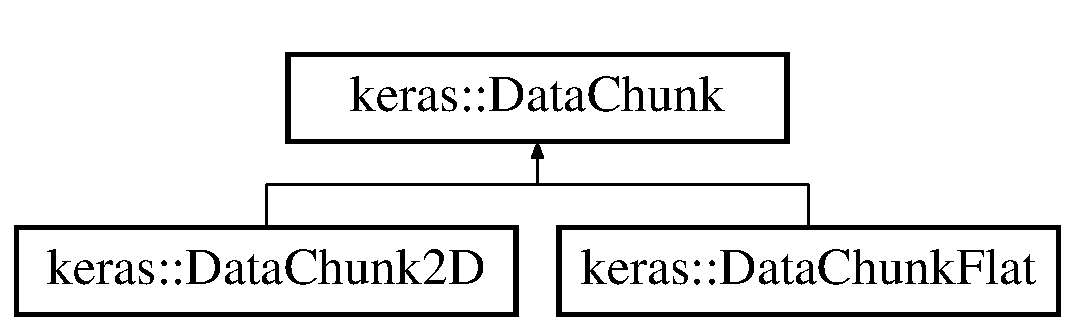
\includegraphics[height=2.000000cm]{classkeras_1_1_data_chunk}
\end{center}
\end{figure}
\subsection*{Public Member Functions}
\begin{DoxyCompactItemize}
\item 
\mbox{\Hypertarget{classkeras_1_1_data_chunk_a5e0df0452c7ae216c3c5fa45f340de7e}\label{classkeras_1_1_data_chunk_a5e0df0452c7ae216c3c5fa45f340de7e}} 
virtual size\+\_\+t {\bfseries get\+\_\+data\+\_\+dim} (void) const
\item 
\mbox{\Hypertarget{classkeras_1_1_data_chunk_ad261b35c28ca2a948609a76c2a32a078}\label{classkeras_1_1_data_chunk_ad261b35c28ca2a948609a76c2a32a078}} 
virtual std\+::vector$<$ double $>$ const  \& {\bfseries get\+\_\+1d} () const
\item 
\mbox{\Hypertarget{classkeras_1_1_data_chunk_a662c5506ecbdb843d88ca5e314956c56}\label{classkeras_1_1_data_chunk_a662c5506ecbdb843d88ca5e314956c56}} 
virtual std\+::vector$<$ std\+::vector$<$ std\+::vector$<$ double $>$ $>$ $>$ const  \& {\bfseries get\+\_\+3d} () const
\item 
\mbox{\Hypertarget{classkeras_1_1_data_chunk_aa7159bb0a04ede97f38f96f183dede1f}\label{classkeras_1_1_data_chunk_aa7159bb0a04ede97f38f96f183dede1f}} 
virtual void {\bfseries set\+\_\+data} (std\+::vector$<$ std\+::vector$<$ std\+::vector$<$ double $>$ $>$ $>$ const \&)
\item 
\mbox{\Hypertarget{classkeras_1_1_data_chunk_abf444fb632f728311dc0560f72a9dfdb}\label{classkeras_1_1_data_chunk_abf444fb632f728311dc0560f72a9dfdb}} 
virtual void {\bfseries set\+\_\+data} (std\+::vector$<$ double $>$ const \&)
\item 
\mbox{\Hypertarget{classkeras_1_1_data_chunk_a26e11e6977aca85141aefd2d304698a4}\label{classkeras_1_1_data_chunk_a26e11e6977aca85141aefd2d304698a4}} 
virtual void {\bfseries read\+\_\+from\+\_\+file} (const std\+::string \&fname)
\item 
\mbox{\Hypertarget{classkeras_1_1_data_chunk_aa34ce27fb36e1c517688f26cc4d95c01}\label{classkeras_1_1_data_chunk_aa34ce27fb36e1c517688f26cc4d95c01}} 
virtual void {\bfseries show\+\_\+name} ()=0
\item 
\mbox{\Hypertarget{classkeras_1_1_data_chunk_a57b1ebfc80d57917c675da96c4894585}\label{classkeras_1_1_data_chunk_a57b1ebfc80d57917c675da96c4894585}} 
virtual void {\bfseries show\+\_\+values} ()=0
\end{DoxyCompactItemize}


The documentation for this class was generated from the following file\+:\begin{DoxyCompactItemize}
\item 
include/\mbox{\hyperlink{keras__model_8hh}{keras\+\_\+model.\+hh}}\end{DoxyCompactItemize}

\hypertarget{classkeras_1_1_data_chunk2_d}{}\section{keras\+:\+:Data\+Chunk2D Class Reference}
\label{classkeras_1_1_data_chunk2_d}\index{keras\+::\+Data\+Chunk2D@{keras\+::\+Data\+Chunk2D}}
Inheritance diagram for keras\+:\+:Data\+Chunk2D\+:\begin{figure}[H]
\begin{center}
\leavevmode
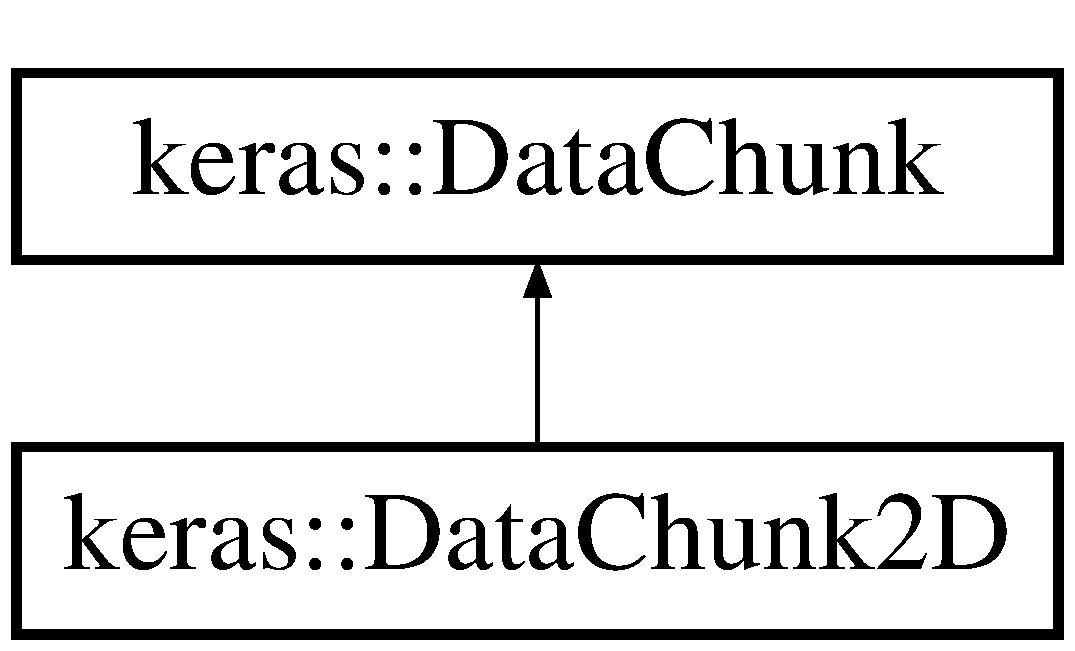
\includegraphics[height=2.000000cm]{classkeras_1_1_data_chunk2_d}
\end{center}
\end{figure}
\subsection*{Public Member Functions}
\begin{DoxyCompactItemize}
\item 
\mbox{\Hypertarget{classkeras_1_1_data_chunk2_d_a03f0b33431723553f2bd05c269d7810f}\label{classkeras_1_1_data_chunk2_d_a03f0b33431723553f2bd05c269d7810f}} 
std\+::vector$<$ std\+::vector$<$ std\+::vector$<$ double $>$ $>$ $>$ const  \& {\bfseries get\+\_\+3d} () const
\item 
\mbox{\Hypertarget{classkeras_1_1_data_chunk2_d_a0a7d7f06553ba90b74a58f12b359dc9e}\label{classkeras_1_1_data_chunk2_d_a0a7d7f06553ba90b74a58f12b359dc9e}} 
virtual void {\bfseries set\+\_\+data} (std\+::vector$<$ std\+::vector$<$ std\+::vector$<$ double $>$ $>$ $>$ const \&d)
\item 
\mbox{\Hypertarget{classkeras_1_1_data_chunk2_d_ac4885f22989d224da813c5b167f3a477}\label{classkeras_1_1_data_chunk2_d_ac4885f22989d224da813c5b167f3a477}} 
size\+\_\+t {\bfseries get\+\_\+data\+\_\+dim} (void) const
\item 
\mbox{\Hypertarget{classkeras_1_1_data_chunk2_d_a177b3b6088e27c39533dea11c044a7a2}\label{classkeras_1_1_data_chunk2_d_a177b3b6088e27c39533dea11c044a7a2}} 
void {\bfseries show\+\_\+name} ()
\item 
\mbox{\Hypertarget{classkeras_1_1_data_chunk2_d_aafff6d495c32e21a807c27990f885dea}\label{classkeras_1_1_data_chunk2_d_aafff6d495c32e21a807c27990f885dea}} 
void {\bfseries show\+\_\+values} ()
\item 
\mbox{\Hypertarget{classkeras_1_1_data_chunk2_d_aaa4e45d73ca87908a0948e4b620b0fb3}\label{classkeras_1_1_data_chunk2_d_aaa4e45d73ca87908a0948e4b620b0fb3}} 
void {\bfseries read\+\_\+from\+\_\+file} (const std\+::string \&fname)
\end{DoxyCompactItemize}
\subsection*{Public Attributes}
\begin{DoxyCompactItemize}
\item 
\mbox{\Hypertarget{classkeras_1_1_data_chunk2_d_af7e21082a12e6e33c41f73cfb7cca94e}\label{classkeras_1_1_data_chunk2_d_af7e21082a12e6e33c41f73cfb7cca94e}} 
std\+::vector$<$ std\+::vector$<$ std\+::vector$<$ double $>$ $>$ $>$ {\bfseries data}
\item 
\mbox{\Hypertarget{classkeras_1_1_data_chunk2_d_a4091feba923b0934a153b48f419fd8f4}\label{classkeras_1_1_data_chunk2_d_a4091feba923b0934a153b48f419fd8f4}} 
int {\bfseries m\+\_\+depth}
\item 
\mbox{\Hypertarget{classkeras_1_1_data_chunk2_d_ab6fe28d4535c6bedb65e3cfd72d6f3a9}\label{classkeras_1_1_data_chunk2_d_ab6fe28d4535c6bedb65e3cfd72d6f3a9}} 
int {\bfseries m\+\_\+rows}
\item 
\mbox{\Hypertarget{classkeras_1_1_data_chunk2_d_a725be452bc01342f51591b115ae1b6e7}\label{classkeras_1_1_data_chunk2_d_a725be452bc01342f51591b115ae1b6e7}} 
int {\bfseries m\+\_\+cols}
\end{DoxyCompactItemize}


The documentation for this class was generated from the following file\+:\begin{DoxyCompactItemize}
\item 
include/\mbox{\hyperlink{keras__model_8hh}{keras\+\_\+model.\+hh}}\end{DoxyCompactItemize}

\hypertarget{classkeras_1_1_data_chunk_flat}{}\section{keras\+:\+:Data\+Chunk\+Flat Class Reference}
\label{classkeras_1_1_data_chunk_flat}\index{keras\+::\+Data\+Chunk\+Flat@{keras\+::\+Data\+Chunk\+Flat}}
Inheritance diagram for keras\+:\+:Data\+Chunk\+Flat\+:\begin{figure}[H]
\begin{center}
\leavevmode
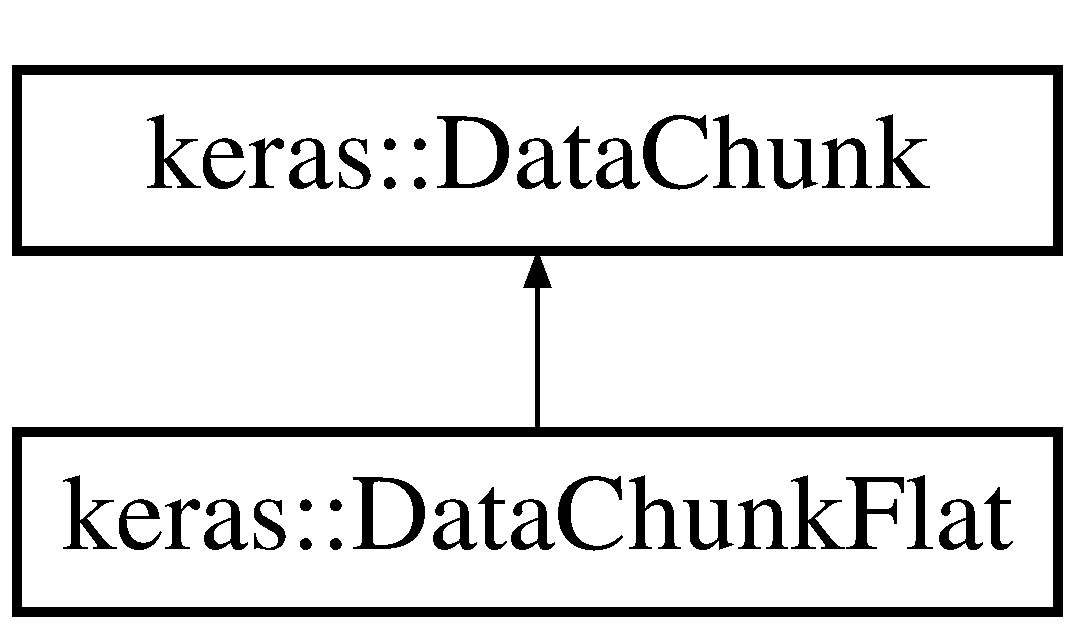
\includegraphics[height=2.000000cm]{classkeras_1_1_data_chunk_flat}
\end{center}
\end{figure}
\subsection*{Public Member Functions}
\begin{DoxyCompactItemize}
\item 
\mbox{\Hypertarget{classkeras_1_1_data_chunk_flat_a23e7ce058e74126bb5c05fd4565c5109}\label{classkeras_1_1_data_chunk_flat_a23e7ce058e74126bb5c05fd4565c5109}} 
{\bfseries Data\+Chunk\+Flat} (size\+\_\+t size)
\item 
\mbox{\Hypertarget{classkeras_1_1_data_chunk_flat_a5b68ee40c3a924fc0e1f0b7a6680284d}\label{classkeras_1_1_data_chunk_flat_a5b68ee40c3a924fc0e1f0b7a6680284d}} 
{\bfseries Data\+Chunk\+Flat} (size\+\_\+t size, double init)
\item 
\mbox{\Hypertarget{classkeras_1_1_data_chunk_flat_ab63f6f87062845bd925a1084b6a979cb}\label{classkeras_1_1_data_chunk_flat_ab63f6f87062845bd925a1084b6a979cb}} 
std\+::vector$<$ double $>$ \& {\bfseries get\+\_\+1d\+\_\+rw} ()
\item 
\mbox{\Hypertarget{classkeras_1_1_data_chunk_flat_addd6d7496d4d2951339a951d54e34173}\label{classkeras_1_1_data_chunk_flat_addd6d7496d4d2951339a951d54e34173}} 
std\+::vector$<$ double $>$ const  \& {\bfseries get\+\_\+1d} () const
\item 
\mbox{\Hypertarget{classkeras_1_1_data_chunk_flat_a7b245c82d49a18fc97b9e20617e958eb}\label{classkeras_1_1_data_chunk_flat_a7b245c82d49a18fc97b9e20617e958eb}} 
void {\bfseries set\+\_\+data} (std\+::vector$<$ double $>$ const \&d)
\item 
\mbox{\Hypertarget{classkeras_1_1_data_chunk_flat_a25bf93e891e64177aa37442780d60078}\label{classkeras_1_1_data_chunk_flat_a25bf93e891e64177aa37442780d60078}} 
size\+\_\+t {\bfseries get\+\_\+data\+\_\+dim} (void) const
\item 
\mbox{\Hypertarget{classkeras_1_1_data_chunk_flat_a50af23bf504327b7c6d3cd0c03c9d81e}\label{classkeras_1_1_data_chunk_flat_a50af23bf504327b7c6d3cd0c03c9d81e}} 
void {\bfseries show\+\_\+name} ()
\item 
\mbox{\Hypertarget{classkeras_1_1_data_chunk_flat_ac1d2d2160dae753e49691531993c42e2}\label{classkeras_1_1_data_chunk_flat_ac1d2d2160dae753e49691531993c42e2}} 
void {\bfseries show\+\_\+values} ()
\item 
\mbox{\Hypertarget{classkeras_1_1_data_chunk_flat_a7ce6915fd2100c555568c00620f74d04}\label{classkeras_1_1_data_chunk_flat_a7ce6915fd2100c555568c00620f74d04}} 
void {\bfseries read\+\_\+from\+\_\+file} (const std\+::string \&fname)
\end{DoxyCompactItemize}
\subsection*{Public Attributes}
\begin{DoxyCompactItemize}
\item 
\mbox{\Hypertarget{classkeras_1_1_data_chunk_flat_abc3a87dfe7305e30116cb21a321583f9}\label{classkeras_1_1_data_chunk_flat_abc3a87dfe7305e30116cb21a321583f9}} 
std\+::vector$<$ double $>$ {\bfseries f}
\end{DoxyCompactItemize}


The documentation for this class was generated from the following file\+:\begin{DoxyCompactItemize}
\item 
include/\mbox{\hyperlink{keras__model_8hh}{keras\+\_\+model.\+hh}}\end{DoxyCompactItemize}

\hypertarget{classerrorx_1_1_data_scaler}{}\section{errorx\+:\+:Data\+Scaler Class Reference}
\label{classerrorx_1_1_data_scaler}\index{errorx\+::\+Data\+Scaler@{errorx\+::\+Data\+Scaler}}
\subsection*{Public Member Functions}
\begin{DoxyCompactItemize}
\item 
\mbox{\hyperlink{classerrorx_1_1_data_scaler_a6a66ab7af20eea46b02f4e193584a038}{Data\+Scaler}} ()
\item 
const vector$<$ double $>$ \mbox{\hyperlink{classerrorx_1_1_data_scaler_accef2aca058fcfdcc27d83dd70a5082d}{scale\+\_\+data}} (vector$<$ double $>$ const \&feature\+\_\+vector)
\end{DoxyCompactItemize}


\subsection{Constructor \& Destructor Documentation}
\mbox{\Hypertarget{classerrorx_1_1_data_scaler_a6a66ab7af20eea46b02f4e193584a038}\label{classerrorx_1_1_data_scaler_a6a66ab7af20eea46b02f4e193584a038}} 
\index{errorx\+::\+Data\+Scaler@{errorx\+::\+Data\+Scaler}!Data\+Scaler@{Data\+Scaler}}
\index{Data\+Scaler@{Data\+Scaler}!errorx\+::\+Data\+Scaler@{errorx\+::\+Data\+Scaler}}
\subsubsection{\texorpdfstring{Data\+Scaler()}{DataScaler()}}
{\footnotesize\ttfamily errorx\+::\+Data\+Scaler\+::\+Data\+Scaler (\begin{DoxyParamCaption}{ }\end{DoxyParamCaption})}

Empty constructor. 

\subsection{Member Function Documentation}
\mbox{\Hypertarget{classerrorx_1_1_data_scaler_accef2aca058fcfdcc27d83dd70a5082d}\label{classerrorx_1_1_data_scaler_accef2aca058fcfdcc27d83dd70a5082d}} 
\index{errorx\+::\+Data\+Scaler@{errorx\+::\+Data\+Scaler}!scale\+\_\+data@{scale\+\_\+data}}
\index{scale\+\_\+data@{scale\+\_\+data}!errorx\+::\+Data\+Scaler@{errorx\+::\+Data\+Scaler}}
\subsubsection{\texorpdfstring{scale\+\_\+data()}{scale\_data()}}
{\footnotesize\ttfamily const vector$<$double$>$ errorx\+::\+Data\+Scaler\+::scale\+\_\+data (\begin{DoxyParamCaption}\item[{vector$<$ double $>$ const \&}]{feature\+\_\+vector }\end{DoxyParamCaption})}

Scales input features to normalize between 0 and 1. Expects feature\+\_\+vector to have 228 entries


\begin{DoxyParams}{Parameters}
{\em feature\+\_\+vector} & features to scale \\
\hline
\end{DoxyParams}


The documentation for this class was generated from the following file\+:\begin{DoxyCompactItemize}
\item 
include/\mbox{\hyperlink{_data_scaler_8hh}{Data\+Scaler.\+hh}}\end{DoxyCompactItemize}

\hypertarget{classerrorx_1_1_error_predictor}{}\section{errorx\+:\+:Error\+Predictor Class Reference}
\label{classerrorx_1_1_error_predictor}\index{errorx\+::\+Error\+Predictor@{errorx\+::\+Error\+Predictor}}
\subsection*{Public Member Functions}
\begin{DoxyCompactItemize}
\item 
\mbox{\hyperlink{classerrorx_1_1_error_predictor_ad00dcb127a4f2e98bbe940271cce277f}{Error\+Predictor}} (int verbose=0)
\item 
\mbox{\hyperlink{classerrorx_1_1_error_predictor_a4604f7bd37aadcad0851d4a2ccfb47f0}{Error\+Predictor}} (\mbox{\hyperlink{classerrorx_1_1_error_predictor}{Error\+Predictor}} const \&other)
\item 
double \mbox{\hyperlink{classerrorx_1_1_error_predictor_a14bf5197cc1ce818fdc5ef44579ad1ef}{apply\+\_\+model}} (\mbox{\hyperlink{classerrorx_1_1_sequence_features}{Sequence\+Features}} const \&features) const
\item 
vector$<$ double $>$ \mbox{\hyperlink{classerrorx_1_1_error_predictor_a9a6b40a5b46466df1a16f904b4b629bb}{apply\+\_\+model}} (vector$<$ vector$<$ double $>$$>$ const features) const
\end{DoxyCompactItemize}


\subsection{Constructor \& Destructor Documentation}
\mbox{\Hypertarget{classerrorx_1_1_error_predictor_ad00dcb127a4f2e98bbe940271cce277f}\label{classerrorx_1_1_error_predictor_ad00dcb127a4f2e98bbe940271cce277f}} 
\index{errorx\+::\+Error\+Predictor@{errorx\+::\+Error\+Predictor}!Error\+Predictor@{Error\+Predictor}}
\index{Error\+Predictor@{Error\+Predictor}!errorx\+::\+Error\+Predictor@{errorx\+::\+Error\+Predictor}}
\subsubsection{\texorpdfstring{Error\+Predictor()}{ErrorPredictor()}\hspace{0.1cm}{\footnotesize\ttfamily [1/2]}}
{\footnotesize\ttfamily errorx\+::\+Error\+Predictor\+::\+Error\+Predictor (\begin{DoxyParamCaption}\item[{int}]{verbose = {\ttfamily 0} }\end{DoxyParamCaption})}

Default constructor \mbox{\Hypertarget{classerrorx_1_1_error_predictor_a4604f7bd37aadcad0851d4a2ccfb47f0}\label{classerrorx_1_1_error_predictor_a4604f7bd37aadcad0851d4a2ccfb47f0}} 
\index{errorx\+::\+Error\+Predictor@{errorx\+::\+Error\+Predictor}!Error\+Predictor@{Error\+Predictor}}
\index{Error\+Predictor@{Error\+Predictor}!errorx\+::\+Error\+Predictor@{errorx\+::\+Error\+Predictor}}
\subsubsection{\texorpdfstring{Error\+Predictor()}{ErrorPredictor()}\hspace{0.1cm}{\footnotesize\ttfamily [2/2]}}
{\footnotesize\ttfamily errorx\+::\+Error\+Predictor\+::\+Error\+Predictor (\begin{DoxyParamCaption}\item[{\mbox{\hyperlink{classerrorx_1_1_error_predictor}{Error\+Predictor}} const \&}]{other }\end{DoxyParamCaption})}

Copy constructor 

\subsection{Member Function Documentation}
\mbox{\Hypertarget{classerrorx_1_1_error_predictor_a14bf5197cc1ce818fdc5ef44579ad1ef}\label{classerrorx_1_1_error_predictor_a14bf5197cc1ce818fdc5ef44579ad1ef}} 
\index{errorx\+::\+Error\+Predictor@{errorx\+::\+Error\+Predictor}!apply\+\_\+model@{apply\+\_\+model}}
\index{apply\+\_\+model@{apply\+\_\+model}!errorx\+::\+Error\+Predictor@{errorx\+::\+Error\+Predictor}}
\subsubsection{\texorpdfstring{apply\+\_\+model()}{apply\_model()}\hspace{0.1cm}{\footnotesize\ttfamily [1/2]}}
{\footnotesize\ttfamily double errorx\+::\+Error\+Predictor\+::apply\+\_\+model (\begin{DoxyParamCaption}\item[{\mbox{\hyperlink{classerrorx_1_1_sequence_features}{Sequence\+Features}} const \&}]{features }\end{DoxyParamCaption}) const}

Applies neural network to features contained in \mbox{\hyperlink{classerrorx_1_1_sequence_features}{Sequence\+Features}} object


\begin{DoxyParams}{Parameters}
{\em features} & \mbox{\hyperlink{classerrorx_1_1_sequence_features}{Sequence\+Features}} object containing features of interest\\
\hline
\end{DoxyParams}
\begin{DoxyReturn}{Returns}
double representing NN prediction for this base 
\end{DoxyReturn}
\mbox{\Hypertarget{classerrorx_1_1_error_predictor_a9a6b40a5b46466df1a16f904b4b629bb}\label{classerrorx_1_1_error_predictor_a9a6b40a5b46466df1a16f904b4b629bb}} 
\index{errorx\+::\+Error\+Predictor@{errorx\+::\+Error\+Predictor}!apply\+\_\+model@{apply\+\_\+model}}
\index{apply\+\_\+model@{apply\+\_\+model}!errorx\+::\+Error\+Predictor@{errorx\+::\+Error\+Predictor}}
\subsubsection{\texorpdfstring{apply\+\_\+model()}{apply\_model()}\hspace{0.1cm}{\footnotesize\ttfamily [2/2]}}
{\footnotesize\ttfamily vector$<$double$>$ errorx\+::\+Error\+Predictor\+::apply\+\_\+model (\begin{DoxyParamCaption}\item[{vector$<$ vector$<$ double $>$$>$ const}]{features }\end{DoxyParamCaption}) const}

Applies neural network to features contained in a vector of double vectors. Expects 228 features per vector


\begin{DoxyParams}{Parameters}
{\em features} & vector of vectors containing features of interest\\
\hline
\end{DoxyParams}
\begin{DoxyReturn}{Returns}
vector of doubles representing NN prediction for each set of features 
\end{DoxyReturn}


The documentation for this class was generated from the following file\+:\begin{DoxyCompactItemize}
\item 
include/\mbox{\hyperlink{_error_predictor_8hh}{Error\+Predictor.\+hh}}\end{DoxyCompactItemize}

\hypertarget{classerrorx_1_1_error_x_options}{}\section{errorx\+:\+:Error\+X\+Options Class Reference}
\label{classerrorx_1_1_error_x_options}\index{errorx\+::\+Error\+X\+Options@{errorx\+::\+Error\+X\+Options}}
\subsection*{Public Member Functions}
\begin{DoxyCompactItemize}
\item 
\mbox{\hyperlink{classerrorx_1_1_error_x_options_afec5f241bdc2f5c4a33ae46437c734e7}{Error\+X\+Options}} ()
\item 
\mbox{\hyperlink{classerrorx_1_1_error_x_options_aa516ca1b14de8755901247249f1f467f}{Error\+X\+Options}} (string infile, string format)
\item 
\mbox{\hyperlink{classerrorx_1_1_error_x_options_a350346cf42cb7349a3975fcc27c51cbd}{Error\+X\+Options}} (\mbox{\hyperlink{classerrorx_1_1_error_x_options}{Error\+X\+Options}} const \&other)
\item 
void \mbox{\hyperlink{classerrorx_1_1_error_x_options_ac45f2c55e8c2dddbbceb5bbdc0acc06f}{fastq\+\_\+to\+\_\+fasta}} ()
\item 
void \mbox{\hyperlink{classerrorx_1_1_error_x_options_a8da4777cb965ad3ef9af136704e4fa62}{validate}} ()
\item 
\mbox{\Hypertarget{classerrorx_1_1_error_x_options_aa1f76c83216f5390f10b6b0594fef709}\label{classerrorx_1_1_error_x_options_aa1f76c83216f5390f10b6b0594fef709}} 
string {\bfseries outfile} () const
\item 
\mbox{\Hypertarget{classerrorx_1_1_error_x_options_a8405ace3a12055908950573263771e21}\label{classerrorx_1_1_error_x_options_a8405ace3a12055908950573263771e21}} 
string {\bfseries format} () const
\item 
\mbox{\Hypertarget{classerrorx_1_1_error_x_options_a1b79f7ab48dc25a4349f0bfb13047204}\label{classerrorx_1_1_error_x_options_a1b79f7ab48dc25a4349f0bfb13047204}} 
string {\bfseries species} () const
\item 
\mbox{\Hypertarget{classerrorx_1_1_error_x_options_aab0542f0e3e8d378bb9bc1e0c8f55884}\label{classerrorx_1_1_error_x_options_aab0542f0e3e8d378bb9bc1e0c8f55884}} 
string {\bfseries infile} () const
\item 
\mbox{\Hypertarget{classerrorx_1_1_error_x_options_aec14f032e11a898359f71fc286c0d45a}\label{classerrorx_1_1_error_x_options_aec14f032e11a898359f71fc286c0d45a}} 
string {\bfseries infasta} () const
\item 
\mbox{\Hypertarget{classerrorx_1_1_error_x_options_acff5f9f2004cbe7605058c9f9b8c5f02}\label{classerrorx_1_1_error_x_options_acff5f9f2004cbe7605058c9f9b8c5f02}} 
string {\bfseries igblast\+\_\+output} () const
\item 
\mbox{\Hypertarget{classerrorx_1_1_error_x_options_a59af9230d2105fbe72692591c002c8e3}\label{classerrorx_1_1_error_x_options_a59af9230d2105fbe72692591c002c8e3}} 
string {\bfseries errorx\+\_\+base} () const
\item 
\mbox{\Hypertarget{classerrorx_1_1_error_x_options_a00dea87538e21313fd0e779dd438ba8f}\label{classerrorx_1_1_error_x_options_a00dea87538e21313fd0e779dd438ba8f}} 
int {\bfseries verbose} () const
\item 
\mbox{\Hypertarget{classerrorx_1_1_error_x_options_a69a164fbc6e6cedb5cdb379234a9477c}\label{classerrorx_1_1_error_x_options_a69a164fbc6e6cedb5cdb379234a9477c}} 
int {\bfseries nthreads} () const
\item 
\mbox{\Hypertarget{classerrorx_1_1_error_x_options_ae55b5b284853f37d1c979ec91d84a830}\label{classerrorx_1_1_error_x_options_ae55b5b284853f37d1c979ec91d84a830}} 
double {\bfseries error\+\_\+threshold} () const
\item 
\mbox{\Hypertarget{classerrorx_1_1_error_x_options_a50083794eea7cc0c2d66b73e7599f43d}\label{classerrorx_1_1_error_x_options_a50083794eea7cc0c2d66b73e7599f43d}} 
char {\bfseries correction} () const
\item 
\mbox{\Hypertarget{classerrorx_1_1_error_x_options_acf5cdf14fdbf602346e4079dc5c94a05}\label{classerrorx_1_1_error_x_options_acf5cdf14fdbf602346e4079dc5c94a05}} 
bool {\bfseries trial} () const
\item 
\mbox{\Hypertarget{classerrorx_1_1_error_x_options_a009d23bcd0f70aa4009fc603d48f2c9b}\label{classerrorx_1_1_error_x_options_a009d23bcd0f70aa4009fc603d48f2c9b}} 
bool {\bfseries allow\+\_\+nonproductive} () const
\item 
\mbox{\Hypertarget{classerrorx_1_1_error_x_options_a533f8b756acb161033cebedd85649875}\label{classerrorx_1_1_error_x_options_a533f8b756acb161033cebedd85649875}} 
void {\bfseries outfile} (string const \&outfile)
\item 
\mbox{\Hypertarget{classerrorx_1_1_error_x_options_a74c4297821f1a27a8b9ca6a9e91edee2}\label{classerrorx_1_1_error_x_options_a74c4297821f1a27a8b9ca6a9e91edee2}} 
void {\bfseries format} (string const \&format)
\item 
\mbox{\Hypertarget{classerrorx_1_1_error_x_options_aeee4c8180711f5699225f236eb00daac}\label{classerrorx_1_1_error_x_options_aeee4c8180711f5699225f236eb00daac}} 
void {\bfseries species} (string const \&species)
\item 
\mbox{\Hypertarget{classerrorx_1_1_error_x_options_a959de3f6891a7d03c89eb754655c508c}\label{classerrorx_1_1_error_x_options_a959de3f6891a7d03c89eb754655c508c}} 
void {\bfseries infile} (string const \&infile)
\item 
\mbox{\Hypertarget{classerrorx_1_1_error_x_options_ab96e7dde52c054b004439a37c24764af}\label{classerrorx_1_1_error_x_options_ab96e7dde52c054b004439a37c24764af}} 
void {\bfseries infasta} (string const \&infasta)
\item 
\mbox{\Hypertarget{classerrorx_1_1_error_x_options_a58c127f03cf3a83806f12340f0fd24f0}\label{classerrorx_1_1_error_x_options_a58c127f03cf3a83806f12340f0fd24f0}} 
void {\bfseries igblast\+\_\+output} (string const \&igblast\+\_\+output)
\item 
\mbox{\Hypertarget{classerrorx_1_1_error_x_options_a69599f3d8575107ad540e10e958d4708}\label{classerrorx_1_1_error_x_options_a69599f3d8575107ad540e10e958d4708}} 
void {\bfseries errorx\+\_\+base} (string const \&errorx\+\_\+base)
\item 
\mbox{\Hypertarget{classerrorx_1_1_error_x_options_aa8af7a4d483d3bec38f53ef538d1e1fb}\label{classerrorx_1_1_error_x_options_aa8af7a4d483d3bec38f53ef538d1e1fb}} 
void {\bfseries verbose} (int const \&verbose)
\item 
\mbox{\Hypertarget{classerrorx_1_1_error_x_options_a597e5ef73f288b1e295ebc14fcff0eee}\label{classerrorx_1_1_error_x_options_a597e5ef73f288b1e295ebc14fcff0eee}} 
void {\bfseries nthreads} (int const \&nthreads)
\item 
\mbox{\Hypertarget{classerrorx_1_1_error_x_options_ac304467292e603cef087a2a2891b4e91}\label{classerrorx_1_1_error_x_options_ac304467292e603cef087a2a2891b4e91}} 
void {\bfseries error\+\_\+threshold} (double const \&error\+\_\+threshold)
\item 
\mbox{\Hypertarget{classerrorx_1_1_error_x_options_adf114f318876400bab0d349b88e67de8}\label{classerrorx_1_1_error_x_options_adf114f318876400bab0d349b88e67de8}} 
void {\bfseries correction} (char const \&correction)
\item 
\mbox{\Hypertarget{classerrorx_1_1_error_x_options_a1a44834413335f68d91021c2f19f445f}\label{classerrorx_1_1_error_x_options_a1a44834413335f68d91021c2f19f445f}} 
void {\bfseries trial} (bool const \&trial)
\item 
\mbox{\Hypertarget{classerrorx_1_1_error_x_options_ac3f5b525e27f2b724efaed80c22349e6}\label{classerrorx_1_1_error_x_options_ac3f5b525e27f2b724efaed80c22349e6}} 
void {\bfseries allow\+\_\+nonproductive} (bool const \&allow\+\_\+nonproductive)
\end{DoxyCompactItemize}


\subsection{Constructor \& Destructor Documentation}
\mbox{\Hypertarget{classerrorx_1_1_error_x_options_afec5f241bdc2f5c4a33ae46437c734e7}\label{classerrorx_1_1_error_x_options_afec5f241bdc2f5c4a33ae46437c734e7}} 
\index{errorx\+::\+Error\+X\+Options@{errorx\+::\+Error\+X\+Options}!Error\+X\+Options@{Error\+X\+Options}}
\index{Error\+X\+Options@{Error\+X\+Options}!errorx\+::\+Error\+X\+Options@{errorx\+::\+Error\+X\+Options}}
\subsubsection{\texorpdfstring{Error\+X\+Options()}{ErrorXOptions()}\hspace{0.1cm}{\footnotesize\ttfamily [1/3]}}
{\footnotesize\ttfamily errorx\+::\+Error\+X\+Options\+::\+Error\+X\+Options (\begin{DoxyParamCaption}{ }\end{DoxyParamCaption})}

Empty constructor. Initializes to default values. Infile and format must be set before using the options though \mbox{\Hypertarget{classerrorx_1_1_error_x_options_aa516ca1b14de8755901247249f1f467f}\label{classerrorx_1_1_error_x_options_aa516ca1b14de8755901247249f1f467f}} 
\index{errorx\+::\+Error\+X\+Options@{errorx\+::\+Error\+X\+Options}!Error\+X\+Options@{Error\+X\+Options}}
\index{Error\+X\+Options@{Error\+X\+Options}!errorx\+::\+Error\+X\+Options@{errorx\+::\+Error\+X\+Options}}
\subsubsection{\texorpdfstring{Error\+X\+Options()}{ErrorXOptions()}\hspace{0.1cm}{\footnotesize\ttfamily [2/3]}}
{\footnotesize\ttfamily errorx\+::\+Error\+X\+Options\+::\+Error\+X\+Options (\begin{DoxyParamCaption}\item[{string}]{infile,  }\item[{string}]{format }\end{DoxyParamCaption})}

Constructor which initializes all to default values, except for required arguments infile and format \mbox{\Hypertarget{classerrorx_1_1_error_x_options_a350346cf42cb7349a3975fcc27c51cbd}\label{classerrorx_1_1_error_x_options_a350346cf42cb7349a3975fcc27c51cbd}} 
\index{errorx\+::\+Error\+X\+Options@{errorx\+::\+Error\+X\+Options}!Error\+X\+Options@{Error\+X\+Options}}
\index{Error\+X\+Options@{Error\+X\+Options}!errorx\+::\+Error\+X\+Options@{errorx\+::\+Error\+X\+Options}}
\subsubsection{\texorpdfstring{Error\+X\+Options()}{ErrorXOptions()}\hspace{0.1cm}{\footnotesize\ttfamily [3/3]}}
{\footnotesize\ttfamily errorx\+::\+Error\+X\+Options\+::\+Error\+X\+Options (\begin{DoxyParamCaption}\item[{\mbox{\hyperlink{classerrorx_1_1_error_x_options}{Error\+X\+Options}} const \&}]{other }\end{DoxyParamCaption})}

Copy constructor 

\subsection{Member Function Documentation}
\mbox{\Hypertarget{classerrorx_1_1_error_x_options_ac45f2c55e8c2dddbbceb5bbdc0acc06f}\label{classerrorx_1_1_error_x_options_ac45f2c55e8c2dddbbceb5bbdc0acc06f}} 
\index{errorx\+::\+Error\+X\+Options@{errorx\+::\+Error\+X\+Options}!fastq\+\_\+to\+\_\+fasta@{fastq\+\_\+to\+\_\+fasta}}
\index{fastq\+\_\+to\+\_\+fasta@{fastq\+\_\+to\+\_\+fasta}!errorx\+::\+Error\+X\+Options@{errorx\+::\+Error\+X\+Options}}
\subsubsection{\texorpdfstring{fastq\+\_\+to\+\_\+fasta()}{fastq\_to\_fasta()}}
{\footnotesize\ttfamily void errorx\+::\+Error\+X\+Options\+::fastq\+\_\+to\+\_\+fasta (\begin{DoxyParamCaption}{ }\end{DoxyParamCaption})}

Converts a F\+A\+S\+TQ file to F\+A\+S\+TA file. Uses the infile\+\_\+ variable to read, and outputs to the same name with the extension .fasta, which is then set to the variable infasta\+\_\+ \mbox{\Hypertarget{classerrorx_1_1_error_x_options_a8da4777cb965ad3ef9af136704e4fa62}\label{classerrorx_1_1_error_x_options_a8da4777cb965ad3ef9af136704e4fa62}} 
\index{errorx\+::\+Error\+X\+Options@{errorx\+::\+Error\+X\+Options}!validate@{validate}}
\index{validate@{validate}!errorx\+::\+Error\+X\+Options@{errorx\+::\+Error\+X\+Options}}
\subsubsection{\texorpdfstring{validate()}{validate()}}
{\footnotesize\ttfamily void errorx\+::\+Error\+X\+Options\+::validate (\begin{DoxyParamCaption}{ }\end{DoxyParamCaption})}

Check that options are properly initialized before running.


\begin{DoxyExceptions}{Exceptions}
{\em invalid\+\_\+argument} & if either infile or format are not specified \\
\hline
\end{DoxyExceptions}


The documentation for this class was generated from the following file\+:\begin{DoxyCompactItemize}
\item 
include/\mbox{\hyperlink{_error_x_options_8hh}{Error\+X\+Options.\+hh}}\end{DoxyCompactItemize}

\hypertarget{classerrorx_1_1_i_g_blast_parser}{}\section{errorx\+:\+:I\+G\+Blast\+Parser Class Reference}
\label{classerrorx_1_1_i_g_blast_parser}\index{errorx\+::\+I\+G\+Blast\+Parser@{errorx\+::\+I\+G\+Blast\+Parser}}
\subsection*{Public Member Functions}
\begin{DoxyCompactItemize}
\item 
\mbox{\hyperlink{classerrorx_1_1_i_g_blast_parser_abae1912dcc92f0dbba19916f5756f3d2}{I\+G\+Blast\+Parser}} ()
\item 
void \mbox{\hyperlink{classerrorx_1_1_i_g_blast_parser_a9b252bb6f6bf829104d6caaf96f776f7}{blast}} (\mbox{\hyperlink{classerrorx_1_1_error_x_options}{Error\+X\+Options}} \&options)
\item 
\mbox{\hyperlink{classerrorx_1_1_sequence_records}{Sequence\+Records}} $\ast$ \mbox{\hyperlink{classerrorx_1_1_i_g_blast_parser_ac5d2a9eb14d830258b9462b1b246fa49}{parse\+\_\+output}} (\mbox{\hyperlink{classerrorx_1_1_error_x_options}{Error\+X\+Options}} \&options)
\end{DoxyCompactItemize}


\subsection{Constructor \& Destructor Documentation}
\mbox{\Hypertarget{classerrorx_1_1_i_g_blast_parser_abae1912dcc92f0dbba19916f5756f3d2}\label{classerrorx_1_1_i_g_blast_parser_abae1912dcc92f0dbba19916f5756f3d2}} 
\index{errorx\+::\+I\+G\+Blast\+Parser@{errorx\+::\+I\+G\+Blast\+Parser}!I\+G\+Blast\+Parser@{I\+G\+Blast\+Parser}}
\index{I\+G\+Blast\+Parser@{I\+G\+Blast\+Parser}!errorx\+::\+I\+G\+Blast\+Parser@{errorx\+::\+I\+G\+Blast\+Parser}}
\subsubsection{\texorpdfstring{I\+G\+Blast\+Parser()}{IGBlastParser()}}
{\footnotesize\ttfamily errorx\+::\+I\+G\+Blast\+Parser\+::\+I\+G\+Blast\+Parser (\begin{DoxyParamCaption}{ }\end{DoxyParamCaption})}

Empty constructor 

\subsection{Member Function Documentation}
\mbox{\Hypertarget{classerrorx_1_1_i_g_blast_parser_a9b252bb6f6bf829104d6caaf96f776f7}\label{classerrorx_1_1_i_g_blast_parser_a9b252bb6f6bf829104d6caaf96f776f7}} 
\index{errorx\+::\+I\+G\+Blast\+Parser@{errorx\+::\+I\+G\+Blast\+Parser}!blast@{blast}}
\index{blast@{blast}!errorx\+::\+I\+G\+Blast\+Parser@{errorx\+::\+I\+G\+Blast\+Parser}}
\subsubsection{\texorpdfstring{blast()}{blast()}}
{\footnotesize\ttfamily void errorx\+::\+I\+G\+Blast\+Parser\+::blast (\begin{DoxyParamCaption}\item[{\mbox{\hyperlink{classerrorx_1_1_error_x_options}{Error\+X\+Options}} \&}]{options }\end{DoxyParamCaption})}

Runs I\+G\+Blast on a set of input sequences based on the information in \mbox{\hyperlink{classerrorx_1_1_error_x_options}{Error\+X\+Options}}


\begin{DoxyParams}{Parameters}
{\em options} & \mbox{\hyperlink{classerrorx_1_1_error_x_options}{Error\+X\+Options}} that dictate what the input and output files are \\
\hline
\end{DoxyParams}
\mbox{\Hypertarget{classerrorx_1_1_i_g_blast_parser_ac5d2a9eb14d830258b9462b1b246fa49}\label{classerrorx_1_1_i_g_blast_parser_ac5d2a9eb14d830258b9462b1b246fa49}} 
\index{errorx\+::\+I\+G\+Blast\+Parser@{errorx\+::\+I\+G\+Blast\+Parser}!parse\+\_\+output@{parse\+\_\+output}}
\index{parse\+\_\+output@{parse\+\_\+output}!errorx\+::\+I\+G\+Blast\+Parser@{errorx\+::\+I\+G\+Blast\+Parser}}
\subsubsection{\texorpdfstring{parse\+\_\+output()}{parse\_output()}}
{\footnotesize\ttfamily \mbox{\hyperlink{classerrorx_1_1_sequence_records}{Sequence\+Records}}$\ast$ errorx\+::\+I\+G\+Blast\+Parser\+::parse\+\_\+output (\begin{DoxyParamCaption}\item[{\mbox{\hyperlink{classerrorx_1_1_error_x_options}{Error\+X\+Options}} \&}]{options }\end{DoxyParamCaption})}

Splits the I\+G\+Blast output file into chunks so that it can be processed and turned into Sequence\+Record(s)


\begin{DoxyParams}{Parameters}
{\em options} & \mbox{\hyperlink{classerrorx_1_1_error_x_options}{Error\+X\+Options}} to control processing\\
\hline
\end{DoxyParams}
\begin{DoxyReturn}{Returns}
A \mbox{\hyperlink{classerrorx_1_1_sequence_records}{Sequence\+Records}} object constructed from the I\+G\+Blast output 
\end{DoxyReturn}


The documentation for this class was generated from the following file\+:\begin{DoxyCompactItemize}
\item 
include/\mbox{\hyperlink{_i_g_blast_parser_8hh}{I\+G\+Blast\+Parser.\+hh}}\end{DoxyCompactItemize}

\hypertarget{classerrorx_1_1_invalid_license_exception}{}\section{errorx\+:\+:Invalid\+License\+Exception Class Reference}
\label{classerrorx_1_1_invalid_license_exception}\index{errorx\+::\+Invalid\+License\+Exception@{errorx\+::\+Invalid\+License\+Exception}}


{\ttfamily \#include $<$exceptions.\+hh$>$}

Inheritance diagram for errorx\+:\+:Invalid\+License\+Exception\+:\begin{figure}[H]
\begin{center}
\leavevmode
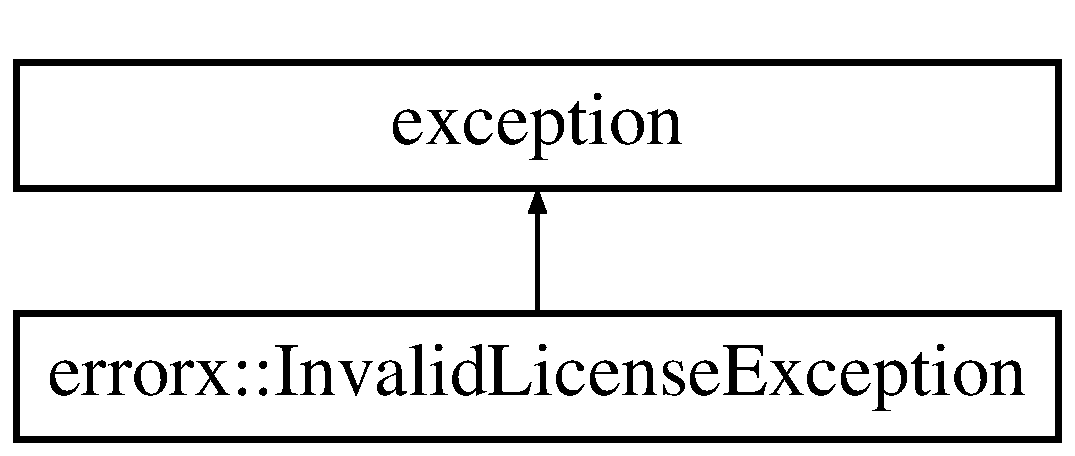
\includegraphics[height=2.000000cm]{classerrorx_1_1_invalid_license_exception}
\end{center}
\end{figure}
\subsection*{Public Member Functions}
\begin{DoxyCompactItemize}
\item 
\mbox{\Hypertarget{classerrorx_1_1_invalid_license_exception_a4887ce2b1956fb57847172088f37b120}\label{classerrorx_1_1_invalid_license_exception_a4887ce2b1956fb57847172088f37b120}} 
const char $\ast$ {\bfseries what} () const  throw ()
\end{DoxyCompactItemize}


\subsection{Detailed Description}
Exception is thrown when there is no valid license file found, and ErrorX is therefore running in trial mode 

The documentation for this class was generated from the following file\+:\begin{DoxyCompactItemize}
\item 
include/\mbox{\hyperlink{exceptions_8hh}{exceptions.\+hh}}\end{DoxyCompactItemize}

\hypertarget{classkeras_1_1_keras_model}{}\section{keras\+:\+:Keras\+Model Class Reference}
\label{classkeras_1_1_keras_model}\index{keras\+::\+Keras\+Model@{keras\+::\+Keras\+Model}}
\subsection*{Public Member Functions}
\begin{DoxyCompactItemize}
\item 
\mbox{\Hypertarget{classkeras_1_1_keras_model_a993a61d91da66f945265d5b960a24ccd}\label{classkeras_1_1_keras_model_a993a61d91da66f945265d5b960a24ccd}} 
{\bfseries Keras\+Model} (const std\+::string \&input\+\_\+fname, int verbose)
\item 
\mbox{\Hypertarget{classkeras_1_1_keras_model_ae9440b0e19b80eca1ef75bd0d6170f77}\label{classkeras_1_1_keras_model_ae9440b0e19b80eca1ef75bd0d6170f77}} 
{\bfseries Keras\+Model} (const std\+::string \&input\+\_\+fname, bool from\+\_\+string, int verbose)
\item 
\mbox{\Hypertarget{classkeras_1_1_keras_model_a6a808591a094dfe3d2b343911d9a488a}\label{classkeras_1_1_keras_model_a6a808591a094dfe3d2b343911d9a488a}} 
std\+::vector$<$ double $>$ {\bfseries compute\+\_\+output} (\mbox{\hyperlink{classkeras_1_1_data_chunk}{keras\+::\+Data\+Chunk}} $\ast$dc) const
\item 
\mbox{\Hypertarget{classkeras_1_1_keras_model_a6132e31054b548fff88e69aeef03ec4f}\label{classkeras_1_1_keras_model_a6132e31054b548fff88e69aeef03ec4f}} 
unsigned int {\bfseries get\+\_\+input\+\_\+rows} () const
\item 
\mbox{\Hypertarget{classkeras_1_1_keras_model_ac73d49ab290d9a4266fac6366a718d3a}\label{classkeras_1_1_keras_model_ac73d49ab290d9a4266fac6366a718d3a}} 
unsigned int {\bfseries get\+\_\+input\+\_\+cols} () const
\item 
\mbox{\Hypertarget{classkeras_1_1_keras_model_a5c6871678cc6053bfe62ded77400463d}\label{classkeras_1_1_keras_model_a5c6871678cc6053bfe62ded77400463d}} 
int {\bfseries get\+\_\+output\+\_\+length} () const
\end{DoxyCompactItemize}


The documentation for this class was generated from the following file\+:\begin{DoxyCompactItemize}
\item 
include/\mbox{\hyperlink{keras__model_8hh}{keras\+\_\+model.\+hh}}\end{DoxyCompactItemize}

\hypertarget{classkeras_1_1_layer}{}\section{keras\+:\+:Layer Class Reference}
\label{classkeras_1_1_layer}\index{keras\+::\+Layer@{keras\+::\+Layer}}
Inheritance diagram for keras\+:\+:Layer\+:\begin{figure}[H]
\begin{center}
\leavevmode
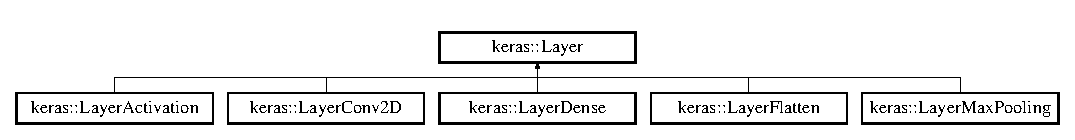
\includegraphics[height=1.435897cm]{classkeras_1_1_layer}
\end{center}
\end{figure}
\subsection*{Public Member Functions}
\begin{DoxyCompactItemize}
\item 
\mbox{\Hypertarget{classkeras_1_1_layer_a591deb80874a90c82fc15e539da01ffd}\label{classkeras_1_1_layer_a591deb80874a90c82fc15e539da01ffd}} 
virtual void {\bfseries load\+\_\+weights} (std\+::ifstream \&fin)=0
\item 
\mbox{\Hypertarget{classkeras_1_1_layer_a3e8c3fa0693580534f3cb1a904382b57}\label{classkeras_1_1_layer_a3e8c3fa0693580534f3cb1a904382b57}} 
virtual void {\bfseries load\+\_\+weights} (std\+::istringstream \&fin)=0
\item 
\mbox{\Hypertarget{classkeras_1_1_layer_a131e3d28719add85c0708f0efecebce8}\label{classkeras_1_1_layer_a131e3d28719add85c0708f0efecebce8}} 
virtual \mbox{\hyperlink{classkeras_1_1_data_chunk}{keras\+::\+Data\+Chunk}} $\ast$ {\bfseries compute\+\_\+output} (\mbox{\hyperlink{classkeras_1_1_data_chunk}{keras\+::\+Data\+Chunk}} $\ast$)=0
\item 
\mbox{\Hypertarget{classkeras_1_1_layer_ab4b6918bd08ac5785bb9d946e2876875}\label{classkeras_1_1_layer_ab4b6918bd08ac5785bb9d946e2876875}} 
{\bfseries Layer} (std\+::string name)
\item 
\mbox{\Hypertarget{classkeras_1_1_layer_a2379da8d9bbe9108304df98b4f4482f4}\label{classkeras_1_1_layer_a2379da8d9bbe9108304df98b4f4482f4}} 
virtual unsigned int {\bfseries get\+\_\+input\+\_\+rows} () const =0
\item 
\mbox{\Hypertarget{classkeras_1_1_layer_a8c4921f448a7fc953e4c3c67a5500e01}\label{classkeras_1_1_layer_a8c4921f448a7fc953e4c3c67a5500e01}} 
virtual unsigned int {\bfseries get\+\_\+input\+\_\+cols} () const =0
\item 
\mbox{\Hypertarget{classkeras_1_1_layer_a5e7c712bf34917d25ace0ff0e2e15f2b}\label{classkeras_1_1_layer_a5e7c712bf34917d25ace0ff0e2e15f2b}} 
virtual unsigned int {\bfseries get\+\_\+output\+\_\+units} () const =0
\item 
\mbox{\Hypertarget{classkeras_1_1_layer_a93467cdf766fb747c300bca9f411900b}\label{classkeras_1_1_layer_a93467cdf766fb747c300bca9f411900b}} 
std\+::string {\bfseries get\+\_\+name} ()
\end{DoxyCompactItemize}
\subsection*{Public Attributes}
\begin{DoxyCompactItemize}
\item 
\mbox{\Hypertarget{classkeras_1_1_layer_a07d82395843bef44049586f33fd9e5a1}\label{classkeras_1_1_layer_a07d82395843bef44049586f33fd9e5a1}} 
std\+::string {\bfseries m\+\_\+name}
\end{DoxyCompactItemize}


The documentation for this class was generated from the following file\+:\begin{DoxyCompactItemize}
\item 
include/\mbox{\hyperlink{keras__model_8hh}{keras\+\_\+model.\+hh}}\end{DoxyCompactItemize}

\hypertarget{classkeras_1_1_layer_activation}{}\section{keras\+:\+:Layer\+Activation Class Reference}
\label{classkeras_1_1_layer_activation}\index{keras\+::\+Layer\+Activation@{keras\+::\+Layer\+Activation}}
Inheritance diagram for keras\+:\+:Layer\+Activation\+:\begin{figure}[H]
\begin{center}
\leavevmode
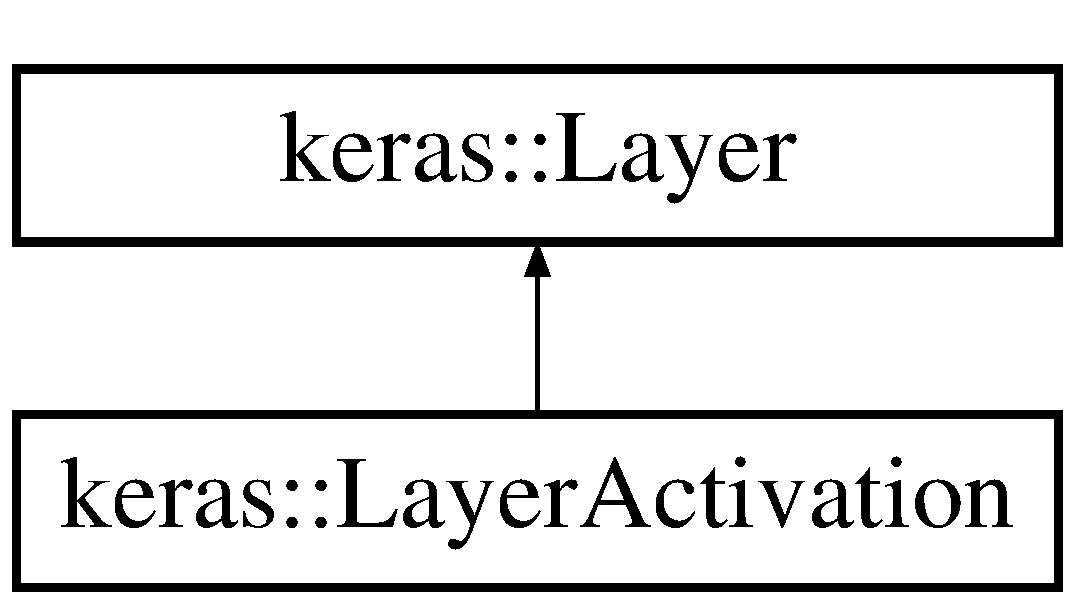
\includegraphics[height=2.000000cm]{classkeras_1_1_layer_activation}
\end{center}
\end{figure}
\subsection*{Public Member Functions}
\begin{DoxyCompactItemize}
\item 
\mbox{\Hypertarget{classkeras_1_1_layer_activation_ab84c8be236ec0a2e09739aa7616463be}\label{classkeras_1_1_layer_activation_ab84c8be236ec0a2e09739aa7616463be}} 
void {\bfseries load\+\_\+weights} (std\+::ifstream \&fin)
\item 
\mbox{\Hypertarget{classkeras_1_1_layer_activation_ae4f3e8ad0c8743e44ec622549cda0861}\label{classkeras_1_1_layer_activation_ae4f3e8ad0c8743e44ec622549cda0861}} 
void {\bfseries load\+\_\+weights} (std\+::istringstream \&fin)
\item 
\mbox{\Hypertarget{classkeras_1_1_layer_activation_a7d3c54078470ed3c46ed56f027d2a933}\label{classkeras_1_1_layer_activation_a7d3c54078470ed3c46ed56f027d2a933}} 
\mbox{\hyperlink{classkeras_1_1_data_chunk}{keras\+::\+Data\+Chunk}} $\ast$ {\bfseries compute\+\_\+output} (\mbox{\hyperlink{classkeras_1_1_data_chunk}{keras\+::\+Data\+Chunk}} $\ast$)
\item 
\mbox{\Hypertarget{classkeras_1_1_layer_activation_a13b37e53a7a9596fdf5054e944fe0667}\label{classkeras_1_1_layer_activation_a13b37e53a7a9596fdf5054e944fe0667}} 
virtual unsigned int {\bfseries get\+\_\+input\+\_\+rows} () const
\item 
\mbox{\Hypertarget{classkeras_1_1_layer_activation_af70e0740fc42167b37486e7e5ebc62ef}\label{classkeras_1_1_layer_activation_af70e0740fc42167b37486e7e5ebc62ef}} 
virtual unsigned int {\bfseries get\+\_\+input\+\_\+cols} () const
\item 
\mbox{\Hypertarget{classkeras_1_1_layer_activation_a7a325387307f8cfb726fff242452211d}\label{classkeras_1_1_layer_activation_a7a325387307f8cfb726fff242452211d}} 
virtual unsigned int {\bfseries get\+\_\+output\+\_\+units} () const
\end{DoxyCompactItemize}
\subsection*{Public Attributes}
\begin{DoxyCompactItemize}
\item 
\mbox{\Hypertarget{classkeras_1_1_layer_activation_ac08c979088c46b5fa5c9319b7081f857}\label{classkeras_1_1_layer_activation_ac08c979088c46b5fa5c9319b7081f857}} 
std\+::string {\bfseries m\+\_\+activation\+\_\+type}
\end{DoxyCompactItemize}


The documentation for this class was generated from the following file\+:\begin{DoxyCompactItemize}
\item 
include/\mbox{\hyperlink{keras__model_8hh}{keras\+\_\+model.\+hh}}\end{DoxyCompactItemize}

\hypertarget{classkeras_1_1_layer_conv2_d}{}\section{keras\+:\+:Layer\+Conv2D Class Reference}
\label{classkeras_1_1_layer_conv2_d}\index{keras\+::\+Layer\+Conv2D@{keras\+::\+Layer\+Conv2D}}
Inheritance diagram for keras\+:\+:Layer\+Conv2D\+:\begin{figure}[H]
\begin{center}
\leavevmode
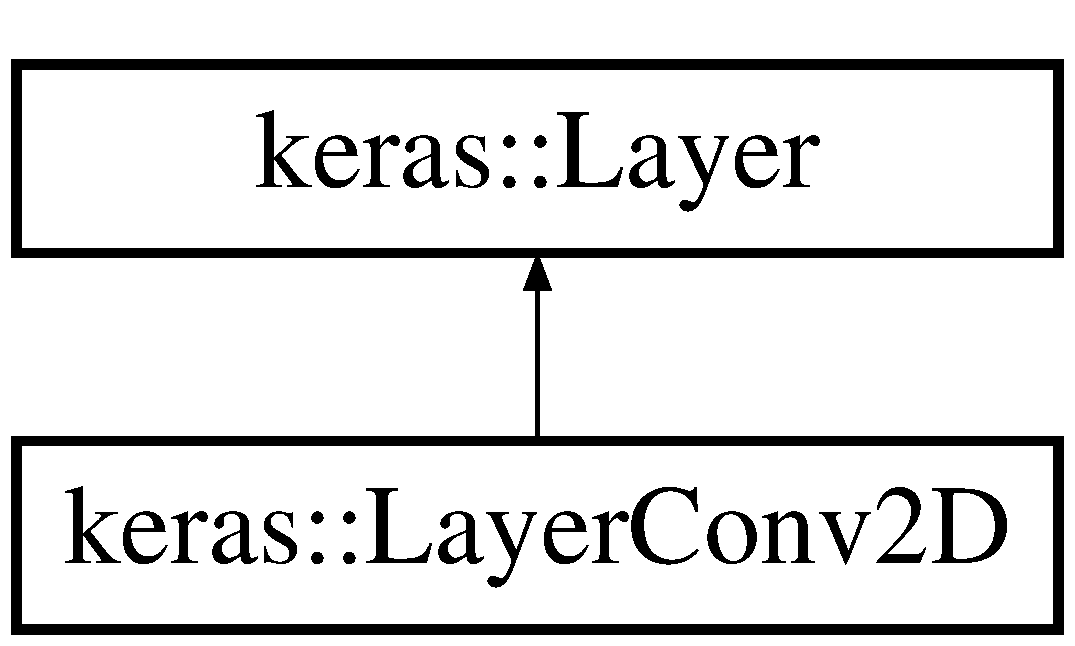
\includegraphics[height=2.000000cm]{classkeras_1_1_layer_conv2_d}
\end{center}
\end{figure}
\subsection*{Public Member Functions}
\begin{DoxyCompactItemize}
\item 
\mbox{\Hypertarget{classkeras_1_1_layer_conv2_d_a210d4bb2d1d1667877acab59c138cb68}\label{classkeras_1_1_layer_conv2_d_a210d4bb2d1d1667877acab59c138cb68}} 
void {\bfseries load\+\_\+weights} (std\+::ifstream \&fin)
\item 
\mbox{\Hypertarget{classkeras_1_1_layer_conv2_d_a8a2811545a58db3d6248fa3e87344c0b}\label{classkeras_1_1_layer_conv2_d_a8a2811545a58db3d6248fa3e87344c0b}} 
void {\bfseries load\+\_\+weights} (std\+::istringstream \&fin)
\item 
\mbox{\Hypertarget{classkeras_1_1_layer_conv2_d_a0615a71c32cf732d4ee6965521c1110a}\label{classkeras_1_1_layer_conv2_d_a0615a71c32cf732d4ee6965521c1110a}} 
\mbox{\hyperlink{classkeras_1_1_data_chunk}{keras\+::\+Data\+Chunk}} $\ast$ {\bfseries compute\+\_\+output} (\mbox{\hyperlink{classkeras_1_1_data_chunk}{keras\+::\+Data\+Chunk}} $\ast$)
\item 
\mbox{\Hypertarget{classkeras_1_1_layer_conv2_d_a2b89ead8620caffc360cbf1a74a31fea}\label{classkeras_1_1_layer_conv2_d_a2b89ead8620caffc360cbf1a74a31fea}} 
virtual unsigned int {\bfseries get\+\_\+input\+\_\+rows} () const
\item 
\mbox{\Hypertarget{classkeras_1_1_layer_conv2_d_ab0bc4c2a6be1dfb536a5118b9aace4a0}\label{classkeras_1_1_layer_conv2_d_ab0bc4c2a6be1dfb536a5118b9aace4a0}} 
virtual unsigned int {\bfseries get\+\_\+input\+\_\+cols} () const
\item 
\mbox{\Hypertarget{classkeras_1_1_layer_conv2_d_a6e57208854c7130737a04b0eb9c5638c}\label{classkeras_1_1_layer_conv2_d_a6e57208854c7130737a04b0eb9c5638c}} 
virtual unsigned int {\bfseries get\+\_\+output\+\_\+units} () const
\end{DoxyCompactItemize}
\subsection*{Public Attributes}
\begin{DoxyCompactItemize}
\item 
\mbox{\Hypertarget{classkeras_1_1_layer_conv2_d_a281eba38468017667fc263f5f398ac64}\label{classkeras_1_1_layer_conv2_d_a281eba38468017667fc263f5f398ac64}} 
std\+::vector$<$ std\+::vector$<$ std\+::vector$<$ std\+::vector$<$ double $>$ $>$ $>$ $>$ {\bfseries m\+\_\+kernels}
\item 
\mbox{\Hypertarget{classkeras_1_1_layer_conv2_d_a2c31ea78bb25fc5e38e9b2759f36b768}\label{classkeras_1_1_layer_conv2_d_a2c31ea78bb25fc5e38e9b2759f36b768}} 
std\+::vector$<$ double $>$ {\bfseries m\+\_\+bias}
\item 
\mbox{\Hypertarget{classkeras_1_1_layer_conv2_d_a1592bb3bcffbbcc8a610c418c289e05f}\label{classkeras_1_1_layer_conv2_d_a1592bb3bcffbbcc8a610c418c289e05f}} 
std\+::string {\bfseries m\+\_\+border\+\_\+mode}
\item 
\mbox{\Hypertarget{classkeras_1_1_layer_conv2_d_ab2e0971eb185b34aa10487b666866194}\label{classkeras_1_1_layer_conv2_d_ab2e0971eb185b34aa10487b666866194}} 
int {\bfseries m\+\_\+kernels\+\_\+cnt}
\item 
\mbox{\Hypertarget{classkeras_1_1_layer_conv2_d_a89695c3b41f2d52253eece3929647dab}\label{classkeras_1_1_layer_conv2_d_a89695c3b41f2d52253eece3929647dab}} 
int {\bfseries m\+\_\+depth}
\item 
\mbox{\Hypertarget{classkeras_1_1_layer_conv2_d_aefaf8276a9171a2dd04e5c94512e549d}\label{classkeras_1_1_layer_conv2_d_aefaf8276a9171a2dd04e5c94512e549d}} 
int {\bfseries m\+\_\+rows}
\item 
\mbox{\Hypertarget{classkeras_1_1_layer_conv2_d_a1ff200ecdc9196e986924a187c22219d}\label{classkeras_1_1_layer_conv2_d_a1ff200ecdc9196e986924a187c22219d}} 
int {\bfseries m\+\_\+cols}
\end{DoxyCompactItemize}


The documentation for this class was generated from the following file\+:\begin{DoxyCompactItemize}
\item 
include/\mbox{\hyperlink{keras__model_8hh}{keras\+\_\+model.\+hh}}\end{DoxyCompactItemize}

\hypertarget{classkeras_1_1_layer_dense}{}\section{keras\+:\+:Layer\+Dense Class Reference}
\label{classkeras_1_1_layer_dense}\index{keras\+::\+Layer\+Dense@{keras\+::\+Layer\+Dense}}
Inheritance diagram for keras\+:\+:Layer\+Dense\+:\begin{figure}[H]
\begin{center}
\leavevmode
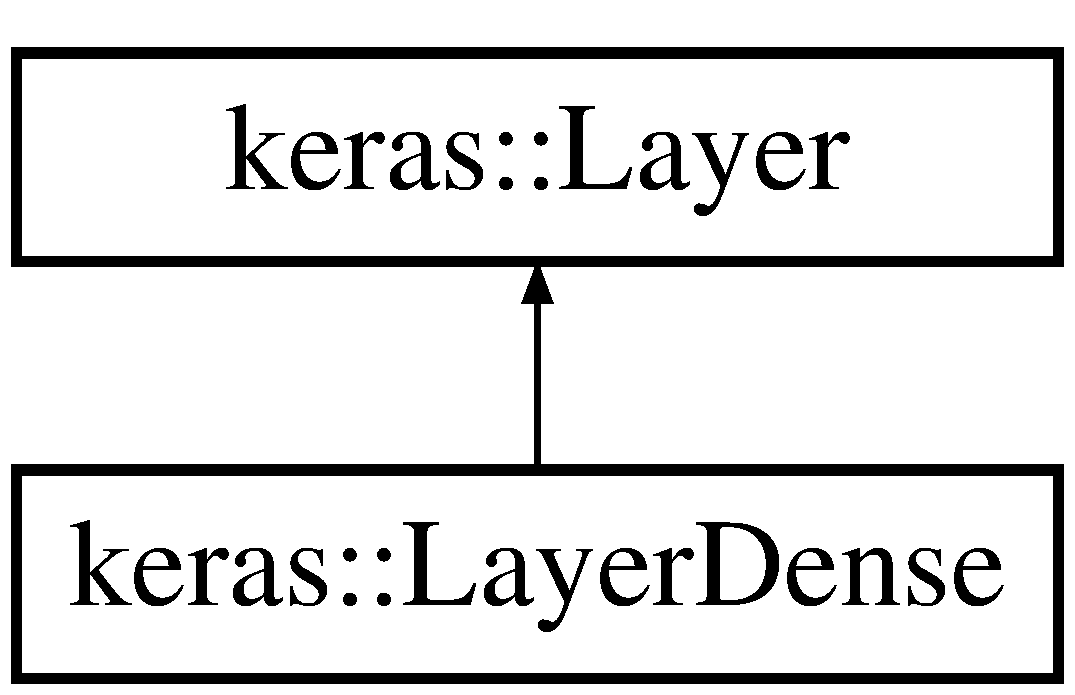
\includegraphics[height=2.000000cm]{classkeras_1_1_layer_dense}
\end{center}
\end{figure}
\subsection*{Public Member Functions}
\begin{DoxyCompactItemize}
\item 
\mbox{\Hypertarget{classkeras_1_1_layer_dense_a780d1734a559d29f3d91a862af17f2d2}\label{classkeras_1_1_layer_dense_a780d1734a559d29f3d91a862af17f2d2}} 
void {\bfseries load\+\_\+weights} (std\+::ifstream \&fin)
\item 
\mbox{\Hypertarget{classkeras_1_1_layer_dense_ae6c3442631bcd63328d6d1a765f48bcd}\label{classkeras_1_1_layer_dense_ae6c3442631bcd63328d6d1a765f48bcd}} 
void {\bfseries load\+\_\+weights} (std\+::istringstream \&fin)
\item 
\mbox{\Hypertarget{classkeras_1_1_layer_dense_a5e3344afb33d9fccd4dd754f264a0a09}\label{classkeras_1_1_layer_dense_a5e3344afb33d9fccd4dd754f264a0a09}} 
\mbox{\hyperlink{classkeras_1_1_data_chunk}{keras\+::\+Data\+Chunk}} $\ast$ {\bfseries compute\+\_\+output} (\mbox{\hyperlink{classkeras_1_1_data_chunk}{keras\+::\+Data\+Chunk}} $\ast$)
\item 
\mbox{\Hypertarget{classkeras_1_1_layer_dense_af7f1e9d3e2fa71d7468a139dd4a00b6c}\label{classkeras_1_1_layer_dense_af7f1e9d3e2fa71d7468a139dd4a00b6c}} 
virtual unsigned int {\bfseries get\+\_\+input\+\_\+rows} () const
\item 
\mbox{\Hypertarget{classkeras_1_1_layer_dense_a75719cba61201688df9bac70736f8c85}\label{classkeras_1_1_layer_dense_a75719cba61201688df9bac70736f8c85}} 
virtual unsigned int {\bfseries get\+\_\+input\+\_\+cols} () const
\item 
\mbox{\Hypertarget{classkeras_1_1_layer_dense_a7cf1d66dba35c1fe9ae493cfd57d829f}\label{classkeras_1_1_layer_dense_a7cf1d66dba35c1fe9ae493cfd57d829f}} 
virtual unsigned int {\bfseries get\+\_\+output\+\_\+units} () const
\item 
\mbox{\Hypertarget{classkeras_1_1_layer_dense_aae095c3b3e7f4bcdae2cd508f37d44a7}\label{classkeras_1_1_layer_dense_aae095c3b3e7f4bcdae2cd508f37d44a7}} 
void {\bfseries print\+\_\+weights} ()
\end{DoxyCompactItemize}
\subsection*{Public Attributes}
\begin{DoxyCompactItemize}
\item 
\mbox{\Hypertarget{classkeras_1_1_layer_dense_a4c37fdf1d48536121eac93d04aa63cbc}\label{classkeras_1_1_layer_dense_a4c37fdf1d48536121eac93d04aa63cbc}} 
std\+::vector$<$ std\+::vector$<$ double $>$ $>$ {\bfseries m\+\_\+weights}
\item 
\mbox{\Hypertarget{classkeras_1_1_layer_dense_a0597e20b719d018b8cdd52c73ae5438d}\label{classkeras_1_1_layer_dense_a0597e20b719d018b8cdd52c73ae5438d}} 
std\+::vector$<$ double $>$ {\bfseries m\+\_\+bias}
\item 
\mbox{\Hypertarget{classkeras_1_1_layer_dense_a27af27cac27ff724ca3bc1406a83dc3f}\label{classkeras_1_1_layer_dense_a27af27cac27ff724ca3bc1406a83dc3f}} 
int {\bfseries m\+\_\+input\+\_\+cnt}
\item 
\mbox{\Hypertarget{classkeras_1_1_layer_dense_a6f2e25a6c4d983f78383a265193ddbb6}\label{classkeras_1_1_layer_dense_a6f2e25a6c4d983f78383a265193ddbb6}} 
int {\bfseries m\+\_\+neurons}
\end{DoxyCompactItemize}


The documentation for this class was generated from the following file\+:\begin{DoxyCompactItemize}
\item 
include/\mbox{\hyperlink{keras__model_8hh}{keras\+\_\+model.\+hh}}\end{DoxyCompactItemize}

\hypertarget{classkeras_1_1_layer_flatten}{}\section{keras\+:\+:Layer\+Flatten Class Reference}
\label{classkeras_1_1_layer_flatten}\index{keras\+::\+Layer\+Flatten@{keras\+::\+Layer\+Flatten}}
Inheritance diagram for keras\+:\+:Layer\+Flatten\+:\begin{figure}[H]
\begin{center}
\leavevmode
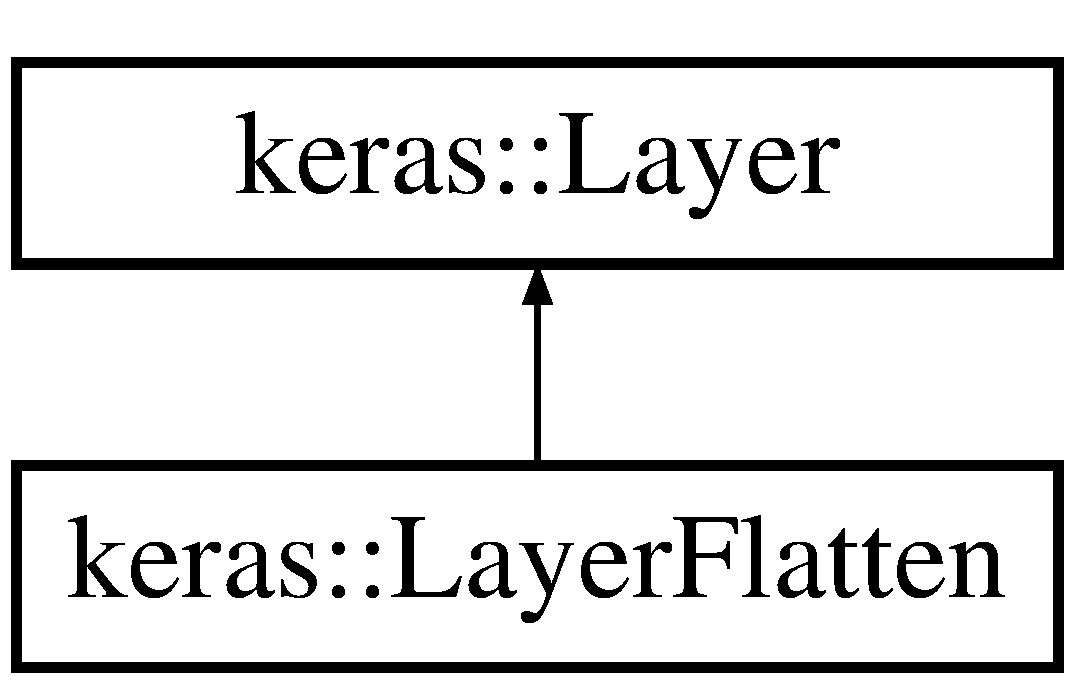
\includegraphics[height=2.000000cm]{classkeras_1_1_layer_flatten}
\end{center}
\end{figure}
\subsection*{Public Member Functions}
\begin{DoxyCompactItemize}
\item 
\mbox{\Hypertarget{classkeras_1_1_layer_flatten_aa936243f0eaf34583fabcfdb5fe1fefa}\label{classkeras_1_1_layer_flatten_aa936243f0eaf34583fabcfdb5fe1fefa}} 
void {\bfseries load\+\_\+weights} (std\+::ifstream \&fin)
\item 
\mbox{\Hypertarget{classkeras_1_1_layer_flatten_a38409a8de78d8858352c271df19090f8}\label{classkeras_1_1_layer_flatten_a38409a8de78d8858352c271df19090f8}} 
void {\bfseries load\+\_\+weights} (std\+::istringstream \&fin)
\item 
\mbox{\Hypertarget{classkeras_1_1_layer_flatten_a0bc9b398a2d47786cbfd74c6fd77bc26}\label{classkeras_1_1_layer_flatten_a0bc9b398a2d47786cbfd74c6fd77bc26}} 
\mbox{\hyperlink{classkeras_1_1_data_chunk}{keras\+::\+Data\+Chunk}} $\ast$ {\bfseries compute\+\_\+output} (\mbox{\hyperlink{classkeras_1_1_data_chunk}{keras\+::\+Data\+Chunk}} $\ast$)
\item 
\mbox{\Hypertarget{classkeras_1_1_layer_flatten_aea54f55b7b342ab2c96417c079023ac7}\label{classkeras_1_1_layer_flatten_aea54f55b7b342ab2c96417c079023ac7}} 
virtual unsigned int {\bfseries get\+\_\+input\+\_\+rows} () const
\item 
\mbox{\Hypertarget{classkeras_1_1_layer_flatten_a896a30c4d1c47abc8c08699b4ea67e11}\label{classkeras_1_1_layer_flatten_a896a30c4d1c47abc8c08699b4ea67e11}} 
virtual unsigned int {\bfseries get\+\_\+input\+\_\+cols} () const
\item 
\mbox{\Hypertarget{classkeras_1_1_layer_flatten_aa579165e501880f3de1938e972077003}\label{classkeras_1_1_layer_flatten_aa579165e501880f3de1938e972077003}} 
virtual unsigned int {\bfseries get\+\_\+output\+\_\+units} () const
\end{DoxyCompactItemize}
\subsection*{Additional Inherited Members}


The documentation for this class was generated from the following file\+:\begin{DoxyCompactItemize}
\item 
include/\mbox{\hyperlink{keras__model_8hh}{keras\+\_\+model.\+hh}}\end{DoxyCompactItemize}

\hypertarget{classkeras_1_1_layer_max_pooling}{}\section{keras\+:\+:Layer\+Max\+Pooling Class Reference}
\label{classkeras_1_1_layer_max_pooling}\index{keras\+::\+Layer\+Max\+Pooling@{keras\+::\+Layer\+Max\+Pooling}}
Inheritance diagram for keras\+:\+:Layer\+Max\+Pooling\+:\begin{figure}[H]
\begin{center}
\leavevmode
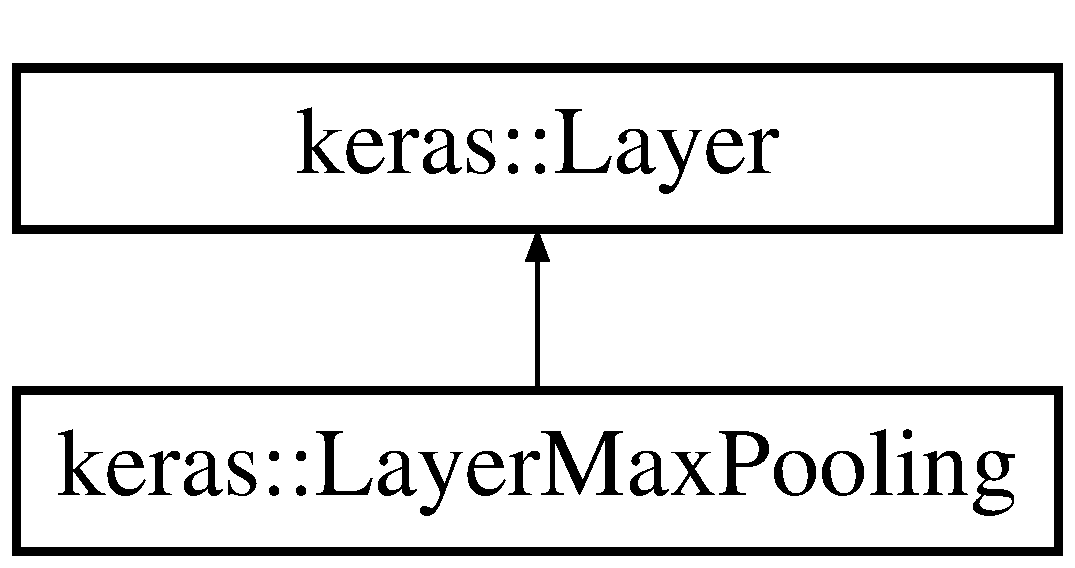
\includegraphics[height=2.000000cm]{classkeras_1_1_layer_max_pooling}
\end{center}
\end{figure}
\subsection*{Public Member Functions}
\begin{DoxyCompactItemize}
\item 
\mbox{\Hypertarget{classkeras_1_1_layer_max_pooling_a2888fe35236b5b548c79b378e117b5c1}\label{classkeras_1_1_layer_max_pooling_a2888fe35236b5b548c79b378e117b5c1}} 
void {\bfseries load\+\_\+weights} (std\+::ifstream \&fin)
\item 
\mbox{\Hypertarget{classkeras_1_1_layer_max_pooling_a3bcaf6af0921ab051abb25fc83f180ca}\label{classkeras_1_1_layer_max_pooling_a3bcaf6af0921ab051abb25fc83f180ca}} 
void {\bfseries load\+\_\+weights} (std\+::istringstream \&fin)
\item 
\mbox{\Hypertarget{classkeras_1_1_layer_max_pooling_a40a3e3a729af250ac7a5dbc6ad60532d}\label{classkeras_1_1_layer_max_pooling_a40a3e3a729af250ac7a5dbc6ad60532d}} 
\mbox{\hyperlink{classkeras_1_1_data_chunk}{keras\+::\+Data\+Chunk}} $\ast$ {\bfseries compute\+\_\+output} (\mbox{\hyperlink{classkeras_1_1_data_chunk}{keras\+::\+Data\+Chunk}} $\ast$)
\item 
\mbox{\Hypertarget{classkeras_1_1_layer_max_pooling_a0161cd63f5d60308511a63c028edcefc}\label{classkeras_1_1_layer_max_pooling_a0161cd63f5d60308511a63c028edcefc}} 
virtual unsigned int {\bfseries get\+\_\+input\+\_\+rows} () const
\item 
\mbox{\Hypertarget{classkeras_1_1_layer_max_pooling_a08040da50a9b2a7ee0bbf54633cf85e6}\label{classkeras_1_1_layer_max_pooling_a08040da50a9b2a7ee0bbf54633cf85e6}} 
virtual unsigned int {\bfseries get\+\_\+input\+\_\+cols} () const
\item 
\mbox{\Hypertarget{classkeras_1_1_layer_max_pooling_ac34fb0e4fa4cf805a45169f1343f9da4}\label{classkeras_1_1_layer_max_pooling_ac34fb0e4fa4cf805a45169f1343f9da4}} 
virtual unsigned int {\bfseries get\+\_\+output\+\_\+units} () const
\end{DoxyCompactItemize}
\subsection*{Public Attributes}
\begin{DoxyCompactItemize}
\item 
\mbox{\Hypertarget{classkeras_1_1_layer_max_pooling_a7cb2748c94a305ecfbd45bef2665f6c7}\label{classkeras_1_1_layer_max_pooling_a7cb2748c94a305ecfbd45bef2665f6c7}} 
int {\bfseries m\+\_\+pool\+\_\+x}
\item 
\mbox{\Hypertarget{classkeras_1_1_layer_max_pooling_a8434bc2ef2f028ad86a7e8f6f22fd5a7}\label{classkeras_1_1_layer_max_pooling_a8434bc2ef2f028ad86a7e8f6f22fd5a7}} 
int {\bfseries m\+\_\+pool\+\_\+y}
\end{DoxyCompactItemize}


The documentation for this class was generated from the following file\+:\begin{DoxyCompactItemize}
\item 
include/\mbox{\hyperlink{keras__model_8hh}{keras\+\_\+model.\+hh}}\end{DoxyCompactItemize}

\hypertarget{classerrorx_1_1_sequence_features}{}\section{errorx\+:\+:Sequence\+Features Class Reference}
\label{classerrorx_1_1_sequence_features}\index{errorx\+::\+Sequence\+Features@{errorx\+::\+Sequence\+Features}}
\subsection*{Public Member Functions}
\begin{DoxyCompactItemize}
\item 
\mbox{\hyperlink{classerrorx_1_1_sequence_features_a5bb9d0bcb3bd6c7877a9902806adc999}{Sequence\+Features}} (\mbox{\hyperlink{classerrorx_1_1_sequence_record}{Sequence\+Record}} $\ast$const record, int position)
\item 
\mbox{\hyperlink{classerrorx_1_1_sequence_features_a56d12eebfb084dc6cb0ce45faf3148ef}{Sequence\+Features}} (\mbox{\hyperlink{classerrorx_1_1_sequence_features}{Sequence\+Features}} const \&other)
\item 
vector$<$ double $>$ \mbox{\hyperlink{classerrorx_1_1_sequence_features_acef9190004088f796ed80cfd32528c47}{get\+\_\+feature\+\_\+vector}} () const
\item 
vector$<$ int $>$ \mbox{\hyperlink{classerrorx_1_1_sequence_features_a3af95ae62f69328d2fec423328130709}{nt\+\_\+to\+\_\+binary}} (char nt) const
\item 
string \mbox{\hyperlink{classerrorx_1_1_sequence_features_a1745dab8123b3da0a8412540ece75b0e}{get\+\_\+window}} (string sequence, int start, int end) const
\item 
\mbox{\Hypertarget{classerrorx_1_1_sequence_features_aef8b453429cc7a18ae9006db84a94d07}\label{classerrorx_1_1_sequence_features_aef8b453429cc7a18ae9006db84a94d07}} 
vector$<$ int $>$ {\bfseries get\+\_\+window} (vector$<$ int $>$ const \&array, int start, int end) const
\item 
vector$<$ int $>$ \mbox{\hyperlink{classerrorx_1_1_sequence_features_aecea6d891f4f91631b8d696882d0af7a}{encode\+\_\+sequence}} (string const \&sequence) const
\item 
bool \mbox{\hyperlink{classerrorx_1_1_sequence_features_a154c6386de18b0200446e4f2e6935296}{is\+\_\+germline}} () const
\end{DoxyCompactItemize}


\subsection{Constructor \& Destructor Documentation}
\mbox{\Hypertarget{classerrorx_1_1_sequence_features_a5bb9d0bcb3bd6c7877a9902806adc999}\label{classerrorx_1_1_sequence_features_a5bb9d0bcb3bd6c7877a9902806adc999}} 
\index{errorx\+::\+Sequence\+Features@{errorx\+::\+Sequence\+Features}!Sequence\+Features@{Sequence\+Features}}
\index{Sequence\+Features@{Sequence\+Features}!errorx\+::\+Sequence\+Features@{errorx\+::\+Sequence\+Features}}
\subsubsection{\texorpdfstring{Sequence\+Features()}{SequenceFeatures()}\hspace{0.1cm}{\footnotesize\ttfamily [1/2]}}
{\footnotesize\ttfamily errorx\+::\+Sequence\+Features\+::\+Sequence\+Features (\begin{DoxyParamCaption}\item[{\mbox{\hyperlink{classerrorx_1_1_sequence_record}{Sequence\+Record}} $\ast$const}]{record,  }\item[{int}]{position }\end{DoxyParamCaption})}

Constructor that uses a \mbox{\hyperlink{classerrorx_1_1_sequence_record}{Sequence\+Record}} object, as well as which position should be predicted as an error.


\begin{DoxyParams}{Parameters}
{\em record} & \mbox{\hyperlink{classerrorx_1_1_sequence_record}{Sequence\+Record}} that contains sequence to be corrected \\
\hline
{\em position} & which position along sequence should be predicted? 0-\/indexed. Should be $<$ record.\+full\+\_\+nt\+\_\+sequence()\\
\hline
\end{DoxyParams}

\begin{DoxyExceptions}{Exceptions}
{\em invalid\+\_\+argument} & if position is out of bounds \\
\hline
\end{DoxyExceptions}
\mbox{\Hypertarget{classerrorx_1_1_sequence_features_a56d12eebfb084dc6cb0ce45faf3148ef}\label{classerrorx_1_1_sequence_features_a56d12eebfb084dc6cb0ce45faf3148ef}} 
\index{errorx\+::\+Sequence\+Features@{errorx\+::\+Sequence\+Features}!Sequence\+Features@{Sequence\+Features}}
\index{Sequence\+Features@{Sequence\+Features}!errorx\+::\+Sequence\+Features@{errorx\+::\+Sequence\+Features}}
\subsubsection{\texorpdfstring{Sequence\+Features()}{SequenceFeatures()}\hspace{0.1cm}{\footnotesize\ttfamily [2/2]}}
{\footnotesize\ttfamily errorx\+::\+Sequence\+Features\+::\+Sequence\+Features (\begin{DoxyParamCaption}\item[{\mbox{\hyperlink{classerrorx_1_1_sequence_features}{Sequence\+Features}} const \&}]{other }\end{DoxyParamCaption})}

Copy constructor 

\subsection{Member Function Documentation}
\mbox{\Hypertarget{classerrorx_1_1_sequence_features_aecea6d891f4f91631b8d696882d0af7a}\label{classerrorx_1_1_sequence_features_aecea6d891f4f91631b8d696882d0af7a}} 
\index{errorx\+::\+Sequence\+Features@{errorx\+::\+Sequence\+Features}!encode\+\_\+sequence@{encode\+\_\+sequence}}
\index{encode\+\_\+sequence@{encode\+\_\+sequence}!errorx\+::\+Sequence\+Features@{errorx\+::\+Sequence\+Features}}
\subsubsection{\texorpdfstring{encode\+\_\+sequence()}{encode\_sequence()}}
{\footnotesize\ttfamily vector$<$int$>$ errorx\+::\+Sequence\+Features\+::encode\+\_\+sequence (\begin{DoxyParamCaption}\item[{string const \&}]{sequence }\end{DoxyParamCaption}) const}

Encode a full NT sequence as a binary vector

\begin{DoxyReturn}{Returns}
sparse binary vector of length 6$\ast$sequence.size() 
\end{DoxyReturn}
\mbox{\Hypertarget{classerrorx_1_1_sequence_features_acef9190004088f796ed80cfd32528c47}\label{classerrorx_1_1_sequence_features_acef9190004088f796ed80cfd32528c47}} 
\index{errorx\+::\+Sequence\+Features@{errorx\+::\+Sequence\+Features}!get\+\_\+feature\+\_\+vector@{get\+\_\+feature\+\_\+vector}}
\index{get\+\_\+feature\+\_\+vector@{get\+\_\+feature\+\_\+vector}!errorx\+::\+Sequence\+Features@{errorx\+::\+Sequence\+Features}}
\subsubsection{\texorpdfstring{get\+\_\+feature\+\_\+vector()}{get\_feature\_vector()}}
{\footnotesize\ttfamily vector$<$double$>$ errorx\+::\+Sequence\+Features\+::get\+\_\+feature\+\_\+vector (\begin{DoxyParamCaption}{ }\end{DoxyParamCaption}) const}

Get the features from this sequence as a vector of length 229

\begin{DoxyReturn}{Returns}
vector of features for NN processing as doubles 
\end{DoxyReturn}
\mbox{\Hypertarget{classerrorx_1_1_sequence_features_a1745dab8123b3da0a8412540ece75b0e}\label{classerrorx_1_1_sequence_features_a1745dab8123b3da0a8412540ece75b0e}} 
\index{errorx\+::\+Sequence\+Features@{errorx\+::\+Sequence\+Features}!get\+\_\+window@{get\+\_\+window}}
\index{get\+\_\+window@{get\+\_\+window}!errorx\+::\+Sequence\+Features@{errorx\+::\+Sequence\+Features}}
\subsubsection{\texorpdfstring{get\+\_\+window()}{get\_window()}}
{\footnotesize\ttfamily string errorx\+::\+Sequence\+Features\+::get\+\_\+window (\begin{DoxyParamCaption}\item[{string}]{sequence,  }\item[{int}]{start,  }\item[{int}]{end }\end{DoxyParamCaption}) const}

Get window surrounding the position of interest. Two functions, either for a string or a vector of ints

\begin{DoxyReturn}{Returns}
string of vector of ints with the surrounding window 
\end{DoxyReturn}
\mbox{\Hypertarget{classerrorx_1_1_sequence_features_a154c6386de18b0200446e4f2e6935296}\label{classerrorx_1_1_sequence_features_a154c6386de18b0200446e4f2e6935296}} 
\index{errorx\+::\+Sequence\+Features@{errorx\+::\+Sequence\+Features}!is\+\_\+germline@{is\+\_\+germline}}
\index{is\+\_\+germline@{is\+\_\+germline}!errorx\+::\+Sequence\+Features@{errorx\+::\+Sequence\+Features}}
\subsubsection{\texorpdfstring{is\+\_\+germline()}{is\_germline()}}
{\footnotesize\ttfamily bool errorx\+::\+Sequence\+Features\+::is\+\_\+germline (\begin{DoxyParamCaption}{ }\end{DoxyParamCaption}) const}

Getter \mbox{\Hypertarget{classerrorx_1_1_sequence_features_a3af95ae62f69328d2fec423328130709}\label{classerrorx_1_1_sequence_features_a3af95ae62f69328d2fec423328130709}} 
\index{errorx\+::\+Sequence\+Features@{errorx\+::\+Sequence\+Features}!nt\+\_\+to\+\_\+binary@{nt\+\_\+to\+\_\+binary}}
\index{nt\+\_\+to\+\_\+binary@{nt\+\_\+to\+\_\+binary}!errorx\+::\+Sequence\+Features@{errorx\+::\+Sequence\+Features}}
\subsubsection{\texorpdfstring{nt\+\_\+to\+\_\+binary()}{nt\_to\_binary()}}
{\footnotesize\ttfamily vector$<$int$>$ errorx\+::\+Sequence\+Features\+::nt\+\_\+to\+\_\+binary (\begin{DoxyParamCaption}\item[{char}]{nt }\end{DoxyParamCaption}) const}

Encode a single NT as a binary vector

\begin{DoxyReturn}{Returns}
sparse binary vector of length 6 
\end{DoxyReturn}


The documentation for this class was generated from the following file\+:\begin{DoxyCompactItemize}
\item 
include/\mbox{\hyperlink{_sequence_features_8hh}{Sequence\+Features.\+hh}}\end{DoxyCompactItemize}

\hypertarget{classerrorx_1_1_sequence_query}{}\section{errorx\+:\+:Sequence\+Query Class Reference}
\label{classerrorx_1_1_sequence_query}\index{errorx\+::\+Sequence\+Query@{errorx\+::\+Sequence\+Query}}
\subsection*{Public Member Functions}
\begin{DoxyCompactItemize}
\item 
\mbox{\hyperlink{classerrorx_1_1_sequence_query_ac09bbe2cd1bfee32d746cd2fcf3bfc45}{Sequence\+Query}} (string \mbox{\hyperlink{classerrorx_1_1_sequence_query_a29c9365ac24b4f46391564b491592394}{sequence\+ID}}, string sequence, string germline\+\_\+sequence, string phred\+\_\+string)
\item 
\mbox{\hyperlink{classerrorx_1_1_sequence_query_af9ec24bc501bcb57431b20f3189cddfc}{Sequence\+Query}} (\mbox{\hyperlink{classerrorx_1_1_sequence_query}{Sequence\+Query}} const \&other)
\item 
void \mbox{\hyperlink{classerrorx_1_1_sequence_query_a29c9365ac24b4f46391564b491592394}{sequence\+ID}} (string const sequence\+ID)
\item 
\mbox{\Hypertarget{classerrorx_1_1_sequence_query_a45fd029e132e8bc62aea50947b269e19}\label{classerrorx_1_1_sequence_query_a45fd029e132e8bc62aea50947b269e19}} 
void {\bfseries sequence} (string const sequence)
\item 
\mbox{\Hypertarget{classerrorx_1_1_sequence_query_a9a4d12a688bfc748f2f15af89244e88a}\label{classerrorx_1_1_sequence_query_a9a4d12a688bfc748f2f15af89244e88a}} 
void {\bfseries germline\+\_\+sequence} (string const germline\+\_\+sequence)
\item 
\mbox{\Hypertarget{classerrorx_1_1_sequence_query_adb9db1b46f6d23f8909d3d6e784fd0aa}\label{classerrorx_1_1_sequence_query_adb9db1b46f6d23f8909d3d6e784fd0aa}} 
void {\bfseries phred\+\_\+string} (string const phred\+\_\+string)
\item 
string \mbox{\hyperlink{classerrorx_1_1_sequence_query_abd2a1128dbdee2be603d130f368bfa32}{sequence\+ID}} () const
\item 
\mbox{\Hypertarget{classerrorx_1_1_sequence_query_a58b4aba456694e71608189ec5d4ff702}\label{classerrorx_1_1_sequence_query_a58b4aba456694e71608189ec5d4ff702}} 
string {\bfseries sequence} () const
\item 
\mbox{\Hypertarget{classerrorx_1_1_sequence_query_a8fef8a62ba11d3610c2fb8311b50fb99}\label{classerrorx_1_1_sequence_query_a8fef8a62ba11d3610c2fb8311b50fb99}} 
string {\bfseries germline\+\_\+sequence} () const
\item 
\mbox{\Hypertarget{classerrorx_1_1_sequence_query_a8459eda44c78b09753ffe3666af2a6a1}\label{classerrorx_1_1_sequence_query_a8459eda44c78b09753ffe3666af2a6a1}} 
string {\bfseries phred\+\_\+string} () const
\end{DoxyCompactItemize}


\subsection{Constructor \& Destructor Documentation}
\mbox{\Hypertarget{classerrorx_1_1_sequence_query_ac09bbe2cd1bfee32d746cd2fcf3bfc45}\label{classerrorx_1_1_sequence_query_ac09bbe2cd1bfee32d746cd2fcf3bfc45}} 
\index{errorx\+::\+Sequence\+Query@{errorx\+::\+Sequence\+Query}!Sequence\+Query@{Sequence\+Query}}
\index{Sequence\+Query@{Sequence\+Query}!errorx\+::\+Sequence\+Query@{errorx\+::\+Sequence\+Query}}
\subsubsection{\texorpdfstring{Sequence\+Query()}{SequenceQuery()}\hspace{0.1cm}{\footnotesize\ttfamily [1/2]}}
{\footnotesize\ttfamily errorx\+::\+Sequence\+Query\+::\+Sequence\+Query (\begin{DoxyParamCaption}\item[{string}]{sequence\+ID,  }\item[{string}]{sequence,  }\item[{string}]{germline\+\_\+sequence,  }\item[{string}]{phred\+\_\+string }\end{DoxyParamCaption})}

Constructor with all the necessary information


\begin{DoxyParams}{Parameters}
{\em sequence\+ID} & Name of sequence \\
\hline
{\em sequence} & NT sequence \\
\hline
{\em germline\+\_\+sequence} & Inferred germline sequence (on D\+NA level) \\
\hline
{\em phred\+\_\+string} & P\+H\+R\+ED (quality) scores straight from the sequencer \\
\hline
\end{DoxyParams}
\mbox{\Hypertarget{classerrorx_1_1_sequence_query_af9ec24bc501bcb57431b20f3189cddfc}\label{classerrorx_1_1_sequence_query_af9ec24bc501bcb57431b20f3189cddfc}} 
\index{errorx\+::\+Sequence\+Query@{errorx\+::\+Sequence\+Query}!Sequence\+Query@{Sequence\+Query}}
\index{Sequence\+Query@{Sequence\+Query}!errorx\+::\+Sequence\+Query@{errorx\+::\+Sequence\+Query}}
\subsubsection{\texorpdfstring{Sequence\+Query()}{SequenceQuery()}\hspace{0.1cm}{\footnotesize\ttfamily [2/2]}}
{\footnotesize\ttfamily errorx\+::\+Sequence\+Query\+::\+Sequence\+Query (\begin{DoxyParamCaption}\item[{\mbox{\hyperlink{classerrorx_1_1_sequence_query}{Sequence\+Query}} const \&}]{other }\end{DoxyParamCaption})}

Copy constructor 

\subsection{Member Function Documentation}
\mbox{\Hypertarget{classerrorx_1_1_sequence_query_a29c9365ac24b4f46391564b491592394}\label{classerrorx_1_1_sequence_query_a29c9365ac24b4f46391564b491592394}} 
\index{errorx\+::\+Sequence\+Query@{errorx\+::\+Sequence\+Query}!sequence\+ID@{sequence\+ID}}
\index{sequence\+ID@{sequence\+ID}!errorx\+::\+Sequence\+Query@{errorx\+::\+Sequence\+Query}}
\subsubsection{\texorpdfstring{sequence\+I\+D()}{sequenceID()}\hspace{0.1cm}{\footnotesize\ttfamily [1/2]}}
{\footnotesize\ttfamily void errorx\+::\+Sequence\+Query\+::sequence\+ID (\begin{DoxyParamCaption}\item[{string const}]{sequence\+ID }\end{DoxyParamCaption})}

Setters \mbox{\Hypertarget{classerrorx_1_1_sequence_query_abd2a1128dbdee2be603d130f368bfa32}\label{classerrorx_1_1_sequence_query_abd2a1128dbdee2be603d130f368bfa32}} 
\index{errorx\+::\+Sequence\+Query@{errorx\+::\+Sequence\+Query}!sequence\+ID@{sequence\+ID}}
\index{sequence\+ID@{sequence\+ID}!errorx\+::\+Sequence\+Query@{errorx\+::\+Sequence\+Query}}
\subsubsection{\texorpdfstring{sequence\+I\+D()}{sequenceID()}\hspace{0.1cm}{\footnotesize\ttfamily [2/2]}}
{\footnotesize\ttfamily string errorx\+::\+Sequence\+Query\+::sequence\+ID (\begin{DoxyParamCaption}{ }\end{DoxyParamCaption}) const}

Getters 

The documentation for this class was generated from the following file\+:\begin{DoxyCompactItemize}
\item 
include/\mbox{\hyperlink{_sequence_query_8hh}{Sequence\+Query.\+hh}}\end{DoxyCompactItemize}

\hypertarget{classerrorx_1_1_sequence_record}{}\section{errorx\+:\+:Sequence\+Record Class Reference}
\label{classerrorx_1_1_sequence_record}\index{errorx\+::\+Sequence\+Record@{errorx\+::\+Sequence\+Record}}
\subsection*{Public Member Functions}
\begin{DoxyCompactItemize}
\item 
\mbox{\hyperlink{classerrorx_1_1_sequence_record_aa0c7da905f4a027969273d7bfe9c2db8}{Sequence\+Record}} ()
\item 
\mbox{\hyperlink{classerrorx_1_1_sequence_record_a659615c7179fdaaaed5196cc37f93623}{Sequence\+Record}} (\mbox{\hyperlink{classerrorx_1_1_sequence_record}{Sequence\+Record}} const \&copy)
\item 
\mbox{\hyperlink{classerrorx_1_1_sequence_record_ac20b7a31e542e34795be7a0450e6d103}{Sequence\+Record}} (vector$<$ string $>$ const \&lines, int verbose=1, bool allow\+\_\+nonproductive=0)
\item 
\mbox{\hyperlink{classerrorx_1_1_sequence_record_a88499ee66ab4eac51eaf51c7c8c8fd2d}{Sequence\+Record}} (\mbox{\hyperlink{classerrorx_1_1_sequence_query}{Sequence\+Query}} \&query, int verbose=1)
\item 
vector$<$ string $>$ \mbox{\hyperlink{classerrorx_1_1_sequence_record_ada8bdfb462b2ba29808b258f4380dbf0}{get\+\_\+summary}} () const
\item 
void \mbox{\hyperlink{classerrorx_1_1_sequence_record_ab6ef0d5067f8c28aee8fb826b7a5922e}{print}} () const
\item 
void \mbox{\hyperlink{classerrorx_1_1_sequence_record_af399cf58824831f8e12247a64108a925}{correct\+\_\+sequence}} (\mbox{\hyperlink{classerrorx_1_1_error_predictor}{Error\+Predictor}} const \&predictor, \mbox{\hyperlink{classerrorx_1_1_error_x_options}{Error\+X\+Options}} const \&options)
\item 
vector$<$ pair$<$ int, double $>$ $>$ \mbox{\hyperlink{classerrorx_1_1_sequence_record_a40aba7774369da0c35b82c14413143a4}{get\+\_\+predicted\+\_\+errors}} ()
\item 
bool \mbox{\hyperlink{classerrorx_1_1_sequence_record_adcc3a75cb5d42ffef94c1c9552fb7c9e}{is\+Good}} ()
\item 
vector$<$ vector$<$ double $>$ $>$ \mbox{\hyperlink{classerrorx_1_1_sequence_record_ac2e7ec6eff313310ba457d9e374b3c88}{get\+\_\+features}} (\mbox{\hyperlink{classerrorx_1_1_error_predictor}{Error\+Predictor}} const \&predictor, \mbox{\hyperlink{classerrorx_1_1_error_x_options}{Error\+X\+Options}} const \&options)
\item 
string \mbox{\hyperlink{classerrorx_1_1_sequence_record_a904548a440ad3da0f4386f55ec7b6eac}{full\+\_\+nt\+\_\+sequence}} () const
\item 
\mbox{\Hypertarget{classerrorx_1_1_sequence_record_a7529518b8da78b2a289a9002bbc3c949}\label{classerrorx_1_1_sequence_record_a7529518b8da78b2a289a9002bbc3c949}} 
string {\bfseries full\+\_\+gl\+\_\+nt\+\_\+sequence} () const
\item 
\mbox{\Hypertarget{classerrorx_1_1_sequence_record_a8cf766707bddbf4b37d09a882aa98574}\label{classerrorx_1_1_sequence_record_a8cf766707bddbf4b37d09a882aa98574}} 
string {\bfseries full\+\_\+nt\+\_\+sequence\+\_\+corrected} () const
\item 
\mbox{\Hypertarget{classerrorx_1_1_sequence_record_a9832ba42ddbad41b3fc5c26f19b84972}\label{classerrorx_1_1_sequence_record_a9832ba42ddbad41b3fc5c26f19b84972}} 
string {\bfseries cdr3\+\_\+aa\+\_\+sequence} () const
\item 
\mbox{\Hypertarget{classerrorx_1_1_sequence_record_a9ea82606e64c7546ae0d18dd78e63d43}\label{classerrorx_1_1_sequence_record_a9ea82606e64c7546ae0d18dd78e63d43}} 
string {\bfseries full\+\_\+aa\+\_\+sequence} () const
\item 
\mbox{\Hypertarget{classerrorx_1_1_sequence_record_aede72d8b08f871d03f75804cdee3065b}\label{classerrorx_1_1_sequence_record_aede72d8b08f871d03f75804cdee3065b}} 
string {\bfseries v\+\_\+gene} () const
\item 
\mbox{\Hypertarget{classerrorx_1_1_sequence_record_a51615c2c2d6612161656eb2f846834eb}\label{classerrorx_1_1_sequence_record_a51615c2c2d6612161656eb2f846834eb}} 
string {\bfseries d\+\_\+gene} () const
\item 
\mbox{\Hypertarget{classerrorx_1_1_sequence_record_a5ffa948395bac606f56c34ec2d8b173b}\label{classerrorx_1_1_sequence_record_a5ffa948395bac606f56c34ec2d8b173b}} 
string {\bfseries j\+\_\+gene} () const
\item 
\mbox{\Hypertarget{classerrorx_1_1_sequence_record_a0ba432d01595ff3ea3faf801b2b8a33f}\label{classerrorx_1_1_sequence_record_a0ba432d01595ff3ea3faf801b2b8a33f}} 
double {\bfseries v\+\_\+identity} () const
\item 
\mbox{\Hypertarget{classerrorx_1_1_sequence_record_a63e683854ad0f25e03f7d024666b1b53}\label{classerrorx_1_1_sequence_record_a63e683854ad0f25e03f7d024666b1b53}} 
double {\bfseries d\+\_\+identity} () const
\item 
\mbox{\Hypertarget{classerrorx_1_1_sequence_record_a64f4d90f07ee89093ce3ad4ce705fa73}\label{classerrorx_1_1_sequence_record_a64f4d90f07ee89093ce3ad4ce705fa73}} 
double {\bfseries j\+\_\+identity} () const
\item 
\mbox{\Hypertarget{classerrorx_1_1_sequence_record_a72c6274059e100c9ea8d94403f9b9992}\label{classerrorx_1_1_sequence_record_a72c6274059e100c9ea8d94403f9b9992}} 
int {\bfseries n\+\_\+errors} () const
\item 
\mbox{\Hypertarget{classerrorx_1_1_sequence_record_ac403cb71ac04931a64738c6c4d7b7f4b}\label{classerrorx_1_1_sequence_record_ac403cb71ac04931a64738c6c4d7b7f4b}} 
string {\bfseries sequence\+ID} () const
\item 
\mbox{\Hypertarget{classerrorx_1_1_sequence_record_ad1544a455cbd242a1f8788cb490c78f3}\label{classerrorx_1_1_sequence_record_ad1544a455cbd242a1f8788cb490c78f3}} 
vector$<$ int $>$ {\bfseries quality\+\_\+array} () const
\item 
\mbox{\Hypertarget{classerrorx_1_1_sequence_record_aaf8830cb13c66a1fb9992596705c0b7e}\label{classerrorx_1_1_sequence_record_aaf8830cb13c66a1fb9992596705c0b7e}} 
int {\bfseries gc\+\_\+count} () const
\item 
\mbox{\Hypertarget{classerrorx_1_1_sequence_record_aec3b2875e607654477e06cdad18d8b92}\label{classerrorx_1_1_sequence_record_aec3b2875e607654477e06cdad18d8b92}} 
double {\bfseries gc\+\_\+pct} () const
\item 
\mbox{\Hypertarget{classerrorx_1_1_sequence_record_aaa4eca015eb95ffbdabeb64b6c7f1a3e}\label{classerrorx_1_1_sequence_record_aaa4eca015eb95ffbdabeb64b6c7f1a3e}} 
double {\bfseries shm} () const
\item 
\mbox{\Hypertarget{classerrorx_1_1_sequence_record_a2ec6f84ad28e2cbbd1d8fbef555c0eef}\label{classerrorx_1_1_sequence_record_a2ec6f84ad28e2cbbd1d8fbef555c0eef}} 
\mbox{\hyperlink{_sequence_record_8hh_a7ec194f8987fd5aa3d34fb5921bff837}{chain\+\_\+type}} {\bfseries chain} () const
\item 
\mbox{\Hypertarget{classerrorx_1_1_sequence_record_a2ce8d5a84e3f305fb3bd8d5bf078b450}\label{classerrorx_1_1_sequence_record_a2ce8d5a84e3f305fb3bd8d5bf078b450}} 
string {\bfseries quality\+\_\+string} () const
\end{DoxyCompactItemize}


\subsection{Constructor \& Destructor Documentation}
\mbox{\Hypertarget{classerrorx_1_1_sequence_record_aa0c7da905f4a027969273d7bfe9c2db8}\label{classerrorx_1_1_sequence_record_aa0c7da905f4a027969273d7bfe9c2db8}} 
\index{errorx\+::\+Sequence\+Record@{errorx\+::\+Sequence\+Record}!Sequence\+Record@{Sequence\+Record}}
\index{Sequence\+Record@{Sequence\+Record}!errorx\+::\+Sequence\+Record@{errorx\+::\+Sequence\+Record}}
\subsubsection{\texorpdfstring{Sequence\+Record()}{SequenceRecord()}\hspace{0.1cm}{\footnotesize\ttfamily [1/4]}}
{\footnotesize\ttfamily errorx\+::\+Sequence\+Record\+::\+Sequence\+Record (\begin{DoxyParamCaption}{ }\end{DoxyParamCaption})}

Empty constructor. Initializes all variables to empty string or 0. \mbox{\Hypertarget{classerrorx_1_1_sequence_record_a659615c7179fdaaaed5196cc37f93623}\label{classerrorx_1_1_sequence_record_a659615c7179fdaaaed5196cc37f93623}} 
\index{errorx\+::\+Sequence\+Record@{errorx\+::\+Sequence\+Record}!Sequence\+Record@{Sequence\+Record}}
\index{Sequence\+Record@{Sequence\+Record}!errorx\+::\+Sequence\+Record@{errorx\+::\+Sequence\+Record}}
\subsubsection{\texorpdfstring{Sequence\+Record()}{SequenceRecord()}\hspace{0.1cm}{\footnotesize\ttfamily [2/4]}}
{\footnotesize\ttfamily errorx\+::\+Sequence\+Record\+::\+Sequence\+Record (\begin{DoxyParamCaption}\item[{\mbox{\hyperlink{classerrorx_1_1_sequence_record}{Sequence\+Record}} const \&}]{copy }\end{DoxyParamCaption})}

Copy constructor. Copies all member variables \mbox{\Hypertarget{classerrorx_1_1_sequence_record_ac20b7a31e542e34795be7a0450e6d103}\label{classerrorx_1_1_sequence_record_ac20b7a31e542e34795be7a0450e6d103}} 
\index{errorx\+::\+Sequence\+Record@{errorx\+::\+Sequence\+Record}!Sequence\+Record@{Sequence\+Record}}
\index{Sequence\+Record@{Sequence\+Record}!errorx\+::\+Sequence\+Record@{errorx\+::\+Sequence\+Record}}
\subsubsection{\texorpdfstring{Sequence\+Record()}{SequenceRecord()}\hspace{0.1cm}{\footnotesize\ttfamily [3/4]}}
{\footnotesize\ttfamily errorx\+::\+Sequence\+Record\+::\+Sequence\+Record (\begin{DoxyParamCaption}\item[{vector$<$ string $>$ const \&}]{lines,  }\item[{int}]{verbose = {\ttfamily 1},  }\item[{bool}]{allow\+\_\+nonproductive = {\ttfamily 0} }\end{DoxyParamCaption})}

Constructs a \mbox{\hyperlink{classerrorx_1_1_sequence_record}{Sequence\+Record}} from a vector of string, representing the lines of an I\+G\+Blast query. Goes through and extracts all information about the sequence by parsing the I\+G\+Blast output.


\begin{DoxyParams}{Parameters}
{\em lines} & vector of string representing lines of I\+G\+Blast query \\
\hline
{\em verbose} & verbosity level to write error messages to the screen? \\
\hline
{\em allow\+\_\+nonproductive} & if a NT sequence is non-\/ productive, still allow it for error correction \\
\hline
\end{DoxyParams}
\mbox{\Hypertarget{classerrorx_1_1_sequence_record_a88499ee66ab4eac51eaf51c7c8c8fd2d}\label{classerrorx_1_1_sequence_record_a88499ee66ab4eac51eaf51c7c8c8fd2d}} 
\index{errorx\+::\+Sequence\+Record@{errorx\+::\+Sequence\+Record}!Sequence\+Record@{Sequence\+Record}}
\index{Sequence\+Record@{Sequence\+Record}!errorx\+::\+Sequence\+Record@{errorx\+::\+Sequence\+Record}}
\subsubsection{\texorpdfstring{Sequence\+Record()}{SequenceRecord()}\hspace{0.1cm}{\footnotesize\ttfamily [4/4]}}
{\footnotesize\ttfamily errorx\+::\+Sequence\+Record\+::\+Sequence\+Record (\begin{DoxyParamCaption}\item[{\mbox{\hyperlink{classerrorx_1_1_sequence_query}{Sequence\+Query}} \&}]{query,  }\item[{int}]{verbose = {\ttfamily 1} }\end{DoxyParamCaption})}

Constructs a \mbox{\hyperlink{classerrorx_1_1_sequence_record}{Sequence\+Record}} from a \mbox{\hyperlink{classerrorx_1_1_sequence_query}{Sequence\+Query}}. The \mbox{\hyperlink{classerrorx_1_1_sequence_query}{Sequence\+Query}} contains only the minimal info needed for error correction, which is sequence ID, NT sequence, germline sequence, and phred score.


\begin{DoxyParams}{Parameters}
{\em query} & \mbox{\hyperlink{classerrorx_1_1_sequence_query}{Sequence\+Query}} object to correct \\
\hline
{\em verbose} & verbosity level to write error messages to the screen? \\
\hline
{\em allow\+\_\+nonproductive} & if a NT sequence is non-\/ productive, still allow it for error correction \\
\hline
\end{DoxyParams}


\subsection{Member Function Documentation}
\mbox{\Hypertarget{classerrorx_1_1_sequence_record_af399cf58824831f8e12247a64108a925}\label{classerrorx_1_1_sequence_record_af399cf58824831f8e12247a64108a925}} 
\index{errorx\+::\+Sequence\+Record@{errorx\+::\+Sequence\+Record}!correct\+\_\+sequence@{correct\+\_\+sequence}}
\index{correct\+\_\+sequence@{correct\+\_\+sequence}!errorx\+::\+Sequence\+Record@{errorx\+::\+Sequence\+Record}}
\subsubsection{\texorpdfstring{correct\+\_\+sequence()}{correct\_sequence()}}
{\footnotesize\ttfamily void errorx\+::\+Sequence\+Record\+::correct\+\_\+sequence (\begin{DoxyParamCaption}\item[{\mbox{\hyperlink{classerrorx_1_1_error_predictor}{Error\+Predictor}} const \&}]{predictor,  }\item[{\mbox{\hyperlink{classerrorx_1_1_error_x_options}{Error\+X\+Options}} const \&}]{options }\end{DoxyParamCaption})}

Correct this \mbox{\hyperlink{classerrorx_1_1_sequence_record}{Sequence\+Record}} and modify in place with the corrected sequence. Params are generally passed by a parent \mbox{\hyperlink{classerrorx_1_1_sequence_records}{Sequence\+Records}} object.


\begin{DoxyParams}{Parameters}
{\em predictor} & \mbox{\hyperlink{classerrorx_1_1_error_predictor}{Error\+Predictor}} for prediction \\
\hline
{\em options} & Options for processing \\
\hline
\end{DoxyParams}
\mbox{\Hypertarget{classerrorx_1_1_sequence_record_a904548a440ad3da0f4386f55ec7b6eac}\label{classerrorx_1_1_sequence_record_a904548a440ad3da0f4386f55ec7b6eac}} 
\index{errorx\+::\+Sequence\+Record@{errorx\+::\+Sequence\+Record}!full\+\_\+nt\+\_\+sequence@{full\+\_\+nt\+\_\+sequence}}
\index{full\+\_\+nt\+\_\+sequence@{full\+\_\+nt\+\_\+sequence}!errorx\+::\+Sequence\+Record@{errorx\+::\+Sequence\+Record}}
\subsubsection{\texorpdfstring{full\+\_\+nt\+\_\+sequence()}{full\_nt\_sequence()}}
{\footnotesize\ttfamily string errorx\+::\+Sequence\+Record\+::full\+\_\+nt\+\_\+sequence (\begin{DoxyParamCaption}{ }\end{DoxyParamCaption}) const}

Getters and setters \mbox{\Hypertarget{classerrorx_1_1_sequence_record_ac2e7ec6eff313310ba457d9e374b3c88}\label{classerrorx_1_1_sequence_record_ac2e7ec6eff313310ba457d9e374b3c88}} 
\index{errorx\+::\+Sequence\+Record@{errorx\+::\+Sequence\+Record}!get\+\_\+features@{get\+\_\+features}}
\index{get\+\_\+features@{get\+\_\+features}!errorx\+::\+Sequence\+Record@{errorx\+::\+Sequence\+Record}}
\subsubsection{\texorpdfstring{get\+\_\+features()}{get\_features()}}
{\footnotesize\ttfamily vector$<$vector$<$double$>$ $>$ errorx\+::\+Sequence\+Record\+::get\+\_\+features (\begin{DoxyParamCaption}\item[{\mbox{\hyperlink{classerrorx_1_1_error_predictor}{Error\+Predictor}} const \&}]{predictor,  }\item[{\mbox{\hyperlink{classerrorx_1_1_error_x_options}{Error\+X\+Options}} const \&}]{options }\end{DoxyParamCaption})}

Get the numeric features associated with this record. Params are generally passed by a parent \mbox{\hyperlink{classerrorx_1_1_sequence_records}{Sequence\+Records}} object.


\begin{DoxyParams}{Parameters}
{\em predictor} & \mbox{\hyperlink{classerrorx_1_1_error_predictor}{Error\+Predictor}} for prediction \\
\hline
{\em options} & Options for processing \\
\hline
\end{DoxyParams}
\mbox{\Hypertarget{classerrorx_1_1_sequence_record_a40aba7774369da0c35b82c14413143a4}\label{classerrorx_1_1_sequence_record_a40aba7774369da0c35b82c14413143a4}} 
\index{errorx\+::\+Sequence\+Record@{errorx\+::\+Sequence\+Record}!get\+\_\+predicted\+\_\+errors@{get\+\_\+predicted\+\_\+errors}}
\index{get\+\_\+predicted\+\_\+errors@{get\+\_\+predicted\+\_\+errors}!errorx\+::\+Sequence\+Record@{errorx\+::\+Sequence\+Record}}
\subsubsection{\texorpdfstring{get\+\_\+predicted\+\_\+errors()}{get\_predicted\_errors()}}
{\footnotesize\ttfamily vector$<$pair$<$int,double$>$ $>$ errorx\+::\+Sequence\+Record\+::get\+\_\+predicted\+\_\+errors (\begin{DoxyParamCaption}{ }\end{DoxyParamCaption})}

Get the predicted probability of error for each base.

\begin{DoxyReturn}{Returns}
vector std\+::pair, where first is the position and second is the probability of error 
\end{DoxyReturn}
\mbox{\Hypertarget{classerrorx_1_1_sequence_record_ada8bdfb462b2ba29808b258f4380dbf0}\label{classerrorx_1_1_sequence_record_ada8bdfb462b2ba29808b258f4380dbf0}} 
\index{errorx\+::\+Sequence\+Record@{errorx\+::\+Sequence\+Record}!get\+\_\+summary@{get\+\_\+summary}}
\index{get\+\_\+summary@{get\+\_\+summary}!errorx\+::\+Sequence\+Record@{errorx\+::\+Sequence\+Record}}
\subsubsection{\texorpdfstring{get\+\_\+summary()}{get\_summary()}}
{\footnotesize\ttfamily vector$<$string$>$ errorx\+::\+Sequence\+Record\+::get\+\_\+summary (\begin{DoxyParamCaption}{ }\end{DoxyParamCaption}) const}

Get all the information summarizing a \mbox{\hyperlink{classerrorx_1_1_sequence_record}{Sequence\+Record}}

\begin{DoxyReturn}{Returns}
vector of strings summarizing the record 
\end{DoxyReturn}
\mbox{\Hypertarget{classerrorx_1_1_sequence_record_adcc3a75cb5d42ffef94c1c9552fb7c9e}\label{classerrorx_1_1_sequence_record_adcc3a75cb5d42ffef94c1c9552fb7c9e}} 
\index{errorx\+::\+Sequence\+Record@{errorx\+::\+Sequence\+Record}!is\+Good@{is\+Good}}
\index{is\+Good@{is\+Good}!errorx\+::\+Sequence\+Record@{errorx\+::\+Sequence\+Record}}
\subsubsection{\texorpdfstring{is\+Good()}{isGood()}}
{\footnotesize\ttfamily bool errorx\+::\+Sequence\+Record\+::is\+Good (\begin{DoxyParamCaption}{ }\end{DoxyParamCaption})}

Return whether this record is \char`\"{}good\char`\"{}. Records can be called \char`\"{}bad\char`\"{} for the following reasons\+:
\begin{DoxyEnumerate}
\item I\+G\+Blast query does not fit the correct format and couldn\textquotesingle{}t be parsed
\item V gene Evalue $>$ 1e-\/3
\item Sequence is not productive (unless allow\+\_\+nonproductive\+\_\+ is True)
\item P\+H\+R\+ED score is not same length as sequence
\end{DoxyEnumerate}

\begin{DoxyReturn}{Returns}
whether sequence is considered good 
\end{DoxyReturn}
\mbox{\Hypertarget{classerrorx_1_1_sequence_record_ab6ef0d5067f8c28aee8fb826b7a5922e}\label{classerrorx_1_1_sequence_record_ab6ef0d5067f8c28aee8fb826b7a5922e}} 
\index{errorx\+::\+Sequence\+Record@{errorx\+::\+Sequence\+Record}!print@{print}}
\index{print@{print}!errorx\+::\+Sequence\+Record@{errorx\+::\+Sequence\+Record}}
\subsubsection{\texorpdfstring{print()}{print()}}
{\footnotesize\ttfamily void errorx\+::\+Sequence\+Record\+::print (\begin{DoxyParamCaption}{ }\end{DoxyParamCaption}) const}

Print key information related to this record 

The documentation for this class was generated from the following file\+:\begin{DoxyCompactItemize}
\item 
include/\mbox{\hyperlink{_sequence_record_8hh}{Sequence\+Record.\+hh}}\end{DoxyCompactItemize}

\hypertarget{classerrorx_1_1_sequence_records}{}\section{errorx\+:\+:Sequence\+Records Class Reference}
\label{classerrorx_1_1_sequence_records}\index{errorx\+::\+Sequence\+Records@{errorx\+::\+Sequence\+Records}}
\subsection*{Public Member Functions}
\begin{DoxyCompactItemize}
\item 
\mbox{\hyperlink{classerrorx_1_1_sequence_records_a0fac9e704c40af45faef33a51b1e160d}{$\sim$\+Sequence\+Records}} ()
\item 
\mbox{\hyperlink{classerrorx_1_1_sequence_records_af45d18ad4ff7f3348289f640e3d6ebca}{Sequence\+Records}} (\mbox{\hyperlink{classerrorx_1_1_error_x_options}{Error\+X\+Options}} const \&options)
\item 
\mbox{\hyperlink{classerrorx_1_1_sequence_records_ae5f0b141e16902f008d5dc65cef492ef}{Sequence\+Records}} (\mbox{\hyperlink{classerrorx_1_1_sequence_records}{Sequence\+Records}} const \&other)
\item 
\mbox{\hyperlink{classerrorx_1_1_sequence_records_a0c868ff30175b97b01beb6239d432603}{Sequence\+Records}} (vector$<$ \mbox{\hyperlink{classerrorx_1_1_sequence_records}{Sequence\+Records}} $\ast$$>$ const \&others)
\item 
\mbox{\hyperlink{classerrorx_1_1_sequence_records_aa5056e29e388a8cc013d304448029a82}{Sequence\+Records}} (vector$<$ \mbox{\hyperlink{classerrorx_1_1_sequence_record}{Sequence\+Record}} $\ast$$>$ const \&record\+\_\+vector, \mbox{\hyperlink{classerrorx_1_1_error_x_options}{Error\+X\+Options}} const \&options)
\item 
void \mbox{\hyperlink{classerrorx_1_1_sequence_records_acc6c04160f2584ae83ed7636104aadaf}{import\+\_\+from\+\_\+tsv}} ()
\item 
void \mbox{\hyperlink{classerrorx_1_1_sequence_records_a3fd1286256f256644c06413bb705df88}{import\+\_\+from\+\_\+list}} (vector$<$ \mbox{\hyperlink{classerrorx_1_1_sequence_query}{Sequence\+Query}} $>$ \&queries)
\item 
float \mbox{\hyperlink{classerrorx_1_1_sequence_records_a84905f56b5cebe34c7300be425964a5b}{estimate\+\_\+error\+\_\+rate}} () const
\item 
void \mbox{\hyperlink{classerrorx_1_1_sequence_records_aae76e748971bbf783b3463be77aa1a3f}{add\+\_\+record}} (\mbox{\hyperlink{classerrorx_1_1_sequence_record}{Sequence\+Record}} $\ast$record)
\item 
int \mbox{\hyperlink{classerrorx_1_1_sequence_records_a3b041b598ce45a217ea229cc5632cc8d}{size}} () const
\item 
vector$<$ \mbox{\hyperlink{classerrorx_1_1_sequence_record}{Sequence\+Record}} $\ast$ $>$ \mbox{\hyperlink{classerrorx_1_1_sequence_records_a9242317332845a8795864556c72ff1e3}{get\+\_\+records}} () const
\item 
\mbox{\hyperlink{classerrorx_1_1_sequence_record}{Sequence\+Record}} $\ast$ \mbox{\hyperlink{classerrorx_1_1_sequence_records_a368bff7f01e34b2d6eedd14c8995d9be}{get}} (int i) const
\item 
int \mbox{\hyperlink{classerrorx_1_1_sequence_records_aa857b90f35804c6f6e179c18033ad838}{good\+\_\+records}} () const
\item 
vector$<$ vector$<$ string $>$ $>$ \mbox{\hyperlink{classerrorx_1_1_sequence_records_a426a62dad84bd4fe3a94a955c7b92330}{get\+\_\+summary}} () const
\item 
vector$<$ string $>$ \mbox{\hyperlink{classerrorx_1_1_sequence_records_a9b65dacacd35715b0ee039843d7d40d0}{get\+\_\+summary\+\_\+labels}} () const
\item 
void \mbox{\hyperlink{classerrorx_1_1_sequence_records_a9bfd2cd859cbdedec5b77c90fd4cbd36}{print\+\_\+summary}} () const
\item 
void \mbox{\hyperlink{classerrorx_1_1_sequence_records_a452c742e8e8b5d2439f2a4de906bd5b7}{write\+\_\+summary}} () const
\item 
void \mbox{\hyperlink{classerrorx_1_1_sequence_records_a7424dd4c03a2f1f4c05307dcd5e5e347}{write\+\_\+features}} ()
\end{DoxyCompactItemize}
\subsection*{Static Public Member Functions}
\begin{DoxyCompactItemize}
\item 
static void \mbox{\hyperlink{classerrorx_1_1_sequence_records_a6df0d323bdcb6f6f570e28fbdf2b6b34}{correct\+\_\+sequences}} (\mbox{\hyperlink{classerrorx_1_1_sequence_records}{Sequence\+Records}} $\ast$\&records)
\end{DoxyCompactItemize}


\subsection{Constructor \& Destructor Documentation}
\mbox{\Hypertarget{classerrorx_1_1_sequence_records_a0fac9e704c40af45faef33a51b1e160d}\label{classerrorx_1_1_sequence_records_a0fac9e704c40af45faef33a51b1e160d}} 
\index{errorx\+::\+Sequence\+Records@{errorx\+::\+Sequence\+Records}!````~Sequence\+Records@{$\sim$\+Sequence\+Records}}
\index{````~Sequence\+Records@{$\sim$\+Sequence\+Records}!errorx\+::\+Sequence\+Records@{errorx\+::\+Sequence\+Records}}
\subsubsection{\texorpdfstring{$\sim$\+Sequence\+Records()}{~SequenceRecords()}}
{\footnotesize\ttfamily errorx\+::\+Sequence\+Records\+::$\sim$\+Sequence\+Records (\begin{DoxyParamCaption}{ }\end{DoxyParamCaption})}

Destructor. Deletes references to member variables options\+\_\+ and predictor\+\_\+. Also deletes references to every \mbox{\hyperlink{classerrorx_1_1_sequence_record}{Sequence\+Record}} contained in records\+\_\+. Every time a \mbox{\hyperlink{classerrorx_1_1_sequence_records}{Sequence\+Records}} object is copied a deep copy is made, so none of these pointers are shared. \mbox{\Hypertarget{classerrorx_1_1_sequence_records_af45d18ad4ff7f3348289f640e3d6ebca}\label{classerrorx_1_1_sequence_records_af45d18ad4ff7f3348289f640e3d6ebca}} 
\index{errorx\+::\+Sequence\+Records@{errorx\+::\+Sequence\+Records}!Sequence\+Records@{Sequence\+Records}}
\index{Sequence\+Records@{Sequence\+Records}!errorx\+::\+Sequence\+Records@{errorx\+::\+Sequence\+Records}}
\subsubsection{\texorpdfstring{Sequence\+Records()}{SequenceRecords()}\hspace{0.1cm}{\footnotesize\ttfamily [1/4]}}
{\footnotesize\ttfamily errorx\+::\+Sequence\+Records\+::\+Sequence\+Records (\begin{DoxyParamCaption}\item[{\mbox{\hyperlink{classerrorx_1_1_error_x_options}{Error\+X\+Options}} const \&}]{options }\end{DoxyParamCaption})}

Constructor using \mbox{\hyperlink{classerrorx_1_1_error_x_options}{Error\+X\+Options}} as argument. \mbox{\Hypertarget{classerrorx_1_1_sequence_records_ae5f0b141e16902f008d5dc65cef492ef}\label{classerrorx_1_1_sequence_records_ae5f0b141e16902f008d5dc65cef492ef}} 
\index{errorx\+::\+Sequence\+Records@{errorx\+::\+Sequence\+Records}!Sequence\+Records@{Sequence\+Records}}
\index{Sequence\+Records@{Sequence\+Records}!errorx\+::\+Sequence\+Records@{errorx\+::\+Sequence\+Records}}
\subsubsection{\texorpdfstring{Sequence\+Records()}{SequenceRecords()}\hspace{0.1cm}{\footnotesize\ttfamily [2/4]}}
{\footnotesize\ttfamily errorx\+::\+Sequence\+Records\+::\+Sequence\+Records (\begin{DoxyParamCaption}\item[{\mbox{\hyperlink{classerrorx_1_1_sequence_records}{Sequence\+Records}} const \&}]{other }\end{DoxyParamCaption})}

Copy constructor. Deep copy of all member variables. \mbox{\Hypertarget{classerrorx_1_1_sequence_records_a0c868ff30175b97b01beb6239d432603}\label{classerrorx_1_1_sequence_records_a0c868ff30175b97b01beb6239d432603}} 
\index{errorx\+::\+Sequence\+Records@{errorx\+::\+Sequence\+Records}!Sequence\+Records@{Sequence\+Records}}
\index{Sequence\+Records@{Sequence\+Records}!errorx\+::\+Sequence\+Records@{errorx\+::\+Sequence\+Records}}
\subsubsection{\texorpdfstring{Sequence\+Records()}{SequenceRecords()}\hspace{0.1cm}{\footnotesize\ttfamily [3/4]}}
{\footnotesize\ttfamily errorx\+::\+Sequence\+Records\+::\+Sequence\+Records (\begin{DoxyParamCaption}\item[{vector$<$ \mbox{\hyperlink{classerrorx_1_1_sequence_records}{Sequence\+Records}} $\ast$$>$ const \&}]{others }\end{DoxyParamCaption})}

Constructor from vector of \mbox{\hyperlink{classerrorx_1_1_sequence_records}{Sequence\+Records}}. Useful for concatenating all of these \mbox{\hyperlink{classerrorx_1_1_sequence_records}{Sequence\+Records}} into a single object. Deep copy of all member variables so they can be safely deleted after. Uses the \mbox{\hyperlink{classerrorx_1_1_error_x_options}{Error\+X\+Options}} member variable from the first item in the vector to get its options. \mbox{\Hypertarget{classerrorx_1_1_sequence_records_aa5056e29e388a8cc013d304448029a82}\label{classerrorx_1_1_sequence_records_aa5056e29e388a8cc013d304448029a82}} 
\index{errorx\+::\+Sequence\+Records@{errorx\+::\+Sequence\+Records}!Sequence\+Records@{Sequence\+Records}}
\index{Sequence\+Records@{Sequence\+Records}!errorx\+::\+Sequence\+Records@{errorx\+::\+Sequence\+Records}}
\subsubsection{\texorpdfstring{Sequence\+Records()}{SequenceRecords()}\hspace{0.1cm}{\footnotesize\ttfamily [4/4]}}
{\footnotesize\ttfamily errorx\+::\+Sequence\+Records\+::\+Sequence\+Records (\begin{DoxyParamCaption}\item[{vector$<$ \mbox{\hyperlink{classerrorx_1_1_sequence_record}{Sequence\+Record}} $\ast$$>$ const \&}]{record\+\_\+vector,  }\item[{\mbox{\hyperlink{classerrorx_1_1_error_x_options}{Error\+X\+Options}} const \&}]{options }\end{DoxyParamCaption})}

Constructor from \mbox{\hyperlink{classerrorx_1_1_sequence_record}{Sequence\+Record}} vector. Useful for concatenating many individual \mbox{\hyperlink{classerrorx_1_1_sequence_record}{Sequence\+Record}} objects into a single object. Deep copy of all member variables so they can be safely deleted after. 

\subsection{Member Function Documentation}
\mbox{\Hypertarget{classerrorx_1_1_sequence_records_aae76e748971bbf783b3463be77aa1a3f}\label{classerrorx_1_1_sequence_records_aae76e748971bbf783b3463be77aa1a3f}} 
\index{errorx\+::\+Sequence\+Records@{errorx\+::\+Sequence\+Records}!add\+\_\+record@{add\+\_\+record}}
\index{add\+\_\+record@{add\+\_\+record}!errorx\+::\+Sequence\+Records@{errorx\+::\+Sequence\+Records}}
\subsubsection{\texorpdfstring{add\+\_\+record()}{add\_record()}}
{\footnotesize\ttfamily void errorx\+::\+Sequence\+Records\+::add\+\_\+record (\begin{DoxyParamCaption}\item[{\mbox{\hyperlink{classerrorx_1_1_sequence_record}{Sequence\+Record}} $\ast$}]{record }\end{DoxyParamCaption})}

Adds a \mbox{\hyperlink{classerrorx_1_1_sequence_record}{Sequence\+Record}} to the records\+\_\+ member variable. Does not copy the record, just assigns it


\begin{DoxyParams}{Parameters}
{\em record} & \mbox{\hyperlink{classerrorx_1_1_sequence_record}{Sequence\+Record}} to add to records\+\_\+ \\
\hline
\end{DoxyParams}
\mbox{\Hypertarget{classerrorx_1_1_sequence_records_a6df0d323bdcb6f6f570e28fbdf2b6b34}\label{classerrorx_1_1_sequence_records_a6df0d323bdcb6f6f570e28fbdf2b6b34}} 
\index{errorx\+::\+Sequence\+Records@{errorx\+::\+Sequence\+Records}!correct\+\_\+sequences@{correct\+\_\+sequences}}
\index{correct\+\_\+sequences@{correct\+\_\+sequences}!errorx\+::\+Sequence\+Records@{errorx\+::\+Sequence\+Records}}
\subsubsection{\texorpdfstring{correct\+\_\+sequences()}{correct\_sequences()}}
{\footnotesize\ttfamily static void errorx\+::\+Sequence\+Records\+::correct\+\_\+sequences (\begin{DoxyParamCaption}\item[{\mbox{\hyperlink{classerrorx_1_1_sequence_records}{Sequence\+Records}} $\ast$\&}]{records }\end{DoxyParamCaption})\hspace{0.3cm}{\ttfamily [static]}}

Runs error correction protocol on each \mbox{\hyperlink{classerrorx_1_1_sequence_record}{Sequence\+Record}} object. Modifies \char`\"{}records\char`\"{} in-\/place. Static qualifier allows it to be used easily in multi-\/threading.


\begin{DoxyParams}{Parameters}
{\em records} & Collection of \mbox{\hyperlink{classerrorx_1_1_sequence_record}{Sequence\+Record}} objects to be error corrected \\
\hline
\end{DoxyParams}
\mbox{\Hypertarget{classerrorx_1_1_sequence_records_a84905f56b5cebe34c7300be425964a5b}\label{classerrorx_1_1_sequence_records_a84905f56b5cebe34c7300be425964a5b}} 
\index{errorx\+::\+Sequence\+Records@{errorx\+::\+Sequence\+Records}!estimate\+\_\+error\+\_\+rate@{estimate\+\_\+error\+\_\+rate}}
\index{estimate\+\_\+error\+\_\+rate@{estimate\+\_\+error\+\_\+rate}!errorx\+::\+Sequence\+Records@{errorx\+::\+Sequence\+Records}}
\subsubsection{\texorpdfstring{estimate\+\_\+error\+\_\+rate()}{estimate\_error\_rate()}}
{\footnotesize\ttfamily float errorx\+::\+Sequence\+Records\+::estimate\+\_\+error\+\_\+rate (\begin{DoxyParamCaption}{ }\end{DoxyParamCaption}) const}

After correcting the member \mbox{\hyperlink{classerrorx_1_1_sequence_record}{Sequence\+Record}} objects, calculates the error rate over the whole set

\begin{DoxyReturn}{Returns}
float value of estimated error rate 
\end{DoxyReturn}
\mbox{\Hypertarget{classerrorx_1_1_sequence_records_a368bff7f01e34b2d6eedd14c8995d9be}\label{classerrorx_1_1_sequence_records_a368bff7f01e34b2d6eedd14c8995d9be}} 
\index{errorx\+::\+Sequence\+Records@{errorx\+::\+Sequence\+Records}!get@{get}}
\index{get@{get}!errorx\+::\+Sequence\+Records@{errorx\+::\+Sequence\+Records}}
\subsubsection{\texorpdfstring{get()}{get()}}
{\footnotesize\ttfamily \mbox{\hyperlink{classerrorx_1_1_sequence_record}{Sequence\+Record}}$\ast$ errorx\+::\+Sequence\+Records\+::get (\begin{DoxyParamCaption}\item[{int}]{i }\end{DoxyParamCaption}) const}

Get a specific \mbox{\hyperlink{classerrorx_1_1_sequence_record}{Sequence\+Record}}


\begin{DoxyParams}{Parameters}
{\em i} & index of desired \mbox{\hyperlink{classerrorx_1_1_sequence_record}{Sequence\+Record}}\\
\hline
\end{DoxyParams}
\begin{DoxyReturn}{Returns}
\mbox{\hyperlink{classerrorx_1_1_sequence_record}{Sequence\+Record}} at index i 
\end{DoxyReturn}
\mbox{\Hypertarget{classerrorx_1_1_sequence_records_a9242317332845a8795864556c72ff1e3}\label{classerrorx_1_1_sequence_records_a9242317332845a8795864556c72ff1e3}} 
\index{errorx\+::\+Sequence\+Records@{errorx\+::\+Sequence\+Records}!get\+\_\+records@{get\+\_\+records}}
\index{get\+\_\+records@{get\+\_\+records}!errorx\+::\+Sequence\+Records@{errorx\+::\+Sequence\+Records}}
\subsubsection{\texorpdfstring{get\+\_\+records()}{get\_records()}}
{\footnotesize\ttfamily vector$<$\mbox{\hyperlink{classerrorx_1_1_sequence_record}{Sequence\+Record}}$\ast$$>$ errorx\+::\+Sequence\+Records\+::get\+\_\+records (\begin{DoxyParamCaption}{ }\end{DoxyParamCaption}) const}

Get the \mbox{\hyperlink{classerrorx_1_1_sequence_record}{Sequence\+Record}} objects held internally

\begin{DoxyReturn}{Returns}
records\+\_\+ member variable 
\end{DoxyReturn}
\mbox{\Hypertarget{classerrorx_1_1_sequence_records_a426a62dad84bd4fe3a94a955c7b92330}\label{classerrorx_1_1_sequence_records_a426a62dad84bd4fe3a94a955c7b92330}} 
\index{errorx\+::\+Sequence\+Records@{errorx\+::\+Sequence\+Records}!get\+\_\+summary@{get\+\_\+summary}}
\index{get\+\_\+summary@{get\+\_\+summary}!errorx\+::\+Sequence\+Records@{errorx\+::\+Sequence\+Records}}
\subsubsection{\texorpdfstring{get\+\_\+summary()}{get\_summary()}}
{\footnotesize\ttfamily vector$<$vector$<$string$>$ $>$ errorx\+::\+Sequence\+Records\+::get\+\_\+summary (\begin{DoxyParamCaption}{ }\end{DoxyParamCaption}) const}

Returns a vector of string vectors, where each string vector is a summary of a \mbox{\hyperlink{classerrorx_1_1_sequence_record}{Sequence\+Record}}

\begin{DoxyReturn}{Returns}
vector of summaries of each \mbox{\hyperlink{classerrorx_1_1_sequence_record}{Sequence\+Record}} 
\end{DoxyReturn}
\mbox{\Hypertarget{classerrorx_1_1_sequence_records_a9b65dacacd35715b0ee039843d7d40d0}\label{classerrorx_1_1_sequence_records_a9b65dacacd35715b0ee039843d7d40d0}} 
\index{errorx\+::\+Sequence\+Records@{errorx\+::\+Sequence\+Records}!get\+\_\+summary\+\_\+labels@{get\+\_\+summary\+\_\+labels}}
\index{get\+\_\+summary\+\_\+labels@{get\+\_\+summary\+\_\+labels}!errorx\+::\+Sequence\+Records@{errorx\+::\+Sequence\+Records}}
\subsubsection{\texorpdfstring{get\+\_\+summary\+\_\+labels()}{get\_summary\_labels()}}
{\footnotesize\ttfamily vector$<$string$>$ errorx\+::\+Sequence\+Records\+::get\+\_\+summary\+\_\+labels (\begin{DoxyParamCaption}{ }\end{DoxyParamCaption}) const}

Returns a vector of labels, where the labels describe the entries from \mbox{\hyperlink{classerrorx_1_1_sequence_records_a426a62dad84bd4fe3a94a955c7b92330}{get\+\_\+summary()}}

\begin{DoxyReturn}{Returns}
vector of labels 
\end{DoxyReturn}
\mbox{\Hypertarget{classerrorx_1_1_sequence_records_aa857b90f35804c6f6e179c18033ad838}\label{classerrorx_1_1_sequence_records_aa857b90f35804c6f6e179c18033ad838}} 
\index{errorx\+::\+Sequence\+Records@{errorx\+::\+Sequence\+Records}!good\+\_\+records@{good\+\_\+records}}
\index{good\+\_\+records@{good\+\_\+records}!errorx\+::\+Sequence\+Records@{errorx\+::\+Sequence\+Records}}
\subsubsection{\texorpdfstring{good\+\_\+records()}{good\_records()}}
{\footnotesize\ttfamily int errorx\+::\+Sequence\+Records\+::good\+\_\+records (\begin{DoxyParamCaption}{ }\end{DoxyParamCaption}) const}

Get number of \char`\"{}good\char`\"{} \mbox{\hyperlink{classerrorx_1_1_sequence_record}{Sequence\+Record}} objects \mbox{\hyperlink{classerrorx_1_1_sequence_records}{Sequence\+Records}} are defined as \char`\"{}good\char`\"{} by the \mbox{\hyperlink{classerrorx_1_1_i_g_blast_parser}{I\+G\+Blast\+Parser}} if they fit certain criteria, such as confident V assignment, productive, etc.

\begin{DoxyReturn}{Returns}
number of \char`\"{}good\char`\"{} records 
\end{DoxyReturn}
\mbox{\Hypertarget{classerrorx_1_1_sequence_records_a3fd1286256f256644c06413bb705df88}\label{classerrorx_1_1_sequence_records_a3fd1286256f256644c06413bb705df88}} 
\index{errorx\+::\+Sequence\+Records@{errorx\+::\+Sequence\+Records}!import\+\_\+from\+\_\+list@{import\+\_\+from\+\_\+list}}
\index{import\+\_\+from\+\_\+list@{import\+\_\+from\+\_\+list}!errorx\+::\+Sequence\+Records@{errorx\+::\+Sequence\+Records}}
\subsubsection{\texorpdfstring{import\+\_\+from\+\_\+list()}{import\_from\_list()}}
{\footnotesize\ttfamily void errorx\+::\+Sequence\+Records\+::import\+\_\+from\+\_\+list (\begin{DoxyParamCaption}\item[{vector$<$ \mbox{\hyperlink{classerrorx_1_1_sequence_query}{Sequence\+Query}} $>$ \&}]{queries }\end{DoxyParamCaption})}

Populates \mbox{\hyperlink{classerrorx_1_1_sequence_records}{Sequence\+Records}} object with elements from a vector of \mbox{\hyperlink{classerrorx_1_1_sequence_query}{Sequence\+Query}} objects


\begin{DoxyParams}{Parameters}
{\em queries} & Vector of \mbox{\hyperlink{classerrorx_1_1_sequence_query}{Sequence\+Query}} objects to use to fill \mbox{\hyperlink{classerrorx_1_1_sequence_records}{Sequence\+Records}} \\
\hline
\end{DoxyParams}
\mbox{\Hypertarget{classerrorx_1_1_sequence_records_acc6c04160f2584ae83ed7636104aadaf}\label{classerrorx_1_1_sequence_records_acc6c04160f2584ae83ed7636104aadaf}} 
\index{errorx\+::\+Sequence\+Records@{errorx\+::\+Sequence\+Records}!import\+\_\+from\+\_\+tsv@{import\+\_\+from\+\_\+tsv}}
\index{import\+\_\+from\+\_\+tsv@{import\+\_\+from\+\_\+tsv}!errorx\+::\+Sequence\+Records@{errorx\+::\+Sequence\+Records}}
\subsubsection{\texorpdfstring{import\+\_\+from\+\_\+tsv()}{import\_from\_tsv()}}
{\footnotesize\ttfamily void errorx\+::\+Sequence\+Records\+::import\+\_\+from\+\_\+tsv (\begin{DoxyParamCaption}{ }\end{DoxyParamCaption})}

Populates \mbox{\hyperlink{classerrorx_1_1_sequence_records}{Sequence\+Records}} object with elements from a T\+SV file. T\+SV file should contain the following columns, in order\+: Sequence\+ID, N\+T\+Sequence, Germline\+Sequence, Phred\+Score \mbox{\Hypertarget{classerrorx_1_1_sequence_records_a9bfd2cd859cbdedec5b77c90fd4cbd36}\label{classerrorx_1_1_sequence_records_a9bfd2cd859cbdedec5b77c90fd4cbd36}} 
\index{errorx\+::\+Sequence\+Records@{errorx\+::\+Sequence\+Records}!print\+\_\+summary@{print\+\_\+summary}}
\index{print\+\_\+summary@{print\+\_\+summary}!errorx\+::\+Sequence\+Records@{errorx\+::\+Sequence\+Records}}
\subsubsection{\texorpdfstring{print\+\_\+summary()}{print\_summary()}}
{\footnotesize\ttfamily void errorx\+::\+Sequence\+Records\+::print\+\_\+summary (\begin{DoxyParamCaption}{ }\end{DoxyParamCaption}) const}

Wraps the \mbox{\hyperlink{classerrorx_1_1_sequence_records_a426a62dad84bd4fe3a94a955c7b92330}{get\+\_\+summary()}} function and writes to std out. \mbox{\Hypertarget{classerrorx_1_1_sequence_records_a3b041b598ce45a217ea229cc5632cc8d}\label{classerrorx_1_1_sequence_records_a3b041b598ce45a217ea229cc5632cc8d}} 
\index{errorx\+::\+Sequence\+Records@{errorx\+::\+Sequence\+Records}!size@{size}}
\index{size@{size}!errorx\+::\+Sequence\+Records@{errorx\+::\+Sequence\+Records}}
\subsubsection{\texorpdfstring{size()}{size()}}
{\footnotesize\ttfamily int errorx\+::\+Sequence\+Records\+::size (\begin{DoxyParamCaption}{ }\end{DoxyParamCaption}) const}

Get the number of \mbox{\hyperlink{classerrorx_1_1_sequence_record}{Sequence\+Record}} objects held internally

\begin{DoxyReturn}{Returns}
size of records\+\_\+ variable 
\end{DoxyReturn}
\mbox{\Hypertarget{classerrorx_1_1_sequence_records_a7424dd4c03a2f1f4c05307dcd5e5e347}\label{classerrorx_1_1_sequence_records_a7424dd4c03a2f1f4c05307dcd5e5e347}} 
\index{errorx\+::\+Sequence\+Records@{errorx\+::\+Sequence\+Records}!write\+\_\+features@{write\+\_\+features}}
\index{write\+\_\+features@{write\+\_\+features}!errorx\+::\+Sequence\+Records@{errorx\+::\+Sequence\+Records}}
\subsubsection{\texorpdfstring{write\+\_\+features()}{write\_features()}}
{\footnotesize\ttfamily void errorx\+::\+Sequence\+Records\+::write\+\_\+features (\begin{DoxyParamCaption}{ }\end{DoxyParamCaption})}

For debugging purposes. Gets features from each \mbox{\hyperlink{classerrorx_1_1_sequence_record}{Sequence\+Record}} object and writes to a file. \mbox{\Hypertarget{classerrorx_1_1_sequence_records_a452c742e8e8b5d2439f2a4de906bd5b7}\label{classerrorx_1_1_sequence_records_a452c742e8e8b5d2439f2a4de906bd5b7}} 
\index{errorx\+::\+Sequence\+Records@{errorx\+::\+Sequence\+Records}!write\+\_\+summary@{write\+\_\+summary}}
\index{write\+\_\+summary@{write\+\_\+summary}!errorx\+::\+Sequence\+Records@{errorx\+::\+Sequence\+Records}}
\subsubsection{\texorpdfstring{write\+\_\+summary()}{write\_summary()}}
{\footnotesize\ttfamily void errorx\+::\+Sequence\+Records\+::write\+\_\+summary (\begin{DoxyParamCaption}{ }\end{DoxyParamCaption}) const}

Wraps the \mbox{\hyperlink{classerrorx_1_1_sequence_records_a426a62dad84bd4fe3a94a955c7b92330}{get\+\_\+summary()}} function and writes to the outfile\+\_\+ variable of \mbox{\hyperlink{classerrorx_1_1_error_x_options}{Error\+X\+Options}}. 

The documentation for this class was generated from the following file\+:\begin{DoxyCompactItemize}
\item 
include/\mbox{\hyperlink{_sequence_records_8hh}{Sequence\+Records.\+hh}}\end{DoxyCompactItemize}

\chapter{File Documentation}
\hypertarget{_data_scaler_8hh}{}\section{include/\+Data\+Scaler.hh File Reference}
\label{_data_scaler_8hh}\index{include/\+Data\+Scaler.\+hh@{include/\+Data\+Scaler.\+hh}}


A simple class to scale features before prediction using a neural network.  


{\ttfamily \#include $<$string$>$}\newline
{\ttfamily \#include $<$vector$>$}\newline
\subsection*{Classes}
\begin{DoxyCompactItemize}
\item 
class \mbox{\hyperlink{classerrorx_1_1_data_scaler}{errorx\+::\+Data\+Scaler}}
\end{DoxyCompactItemize}


\subsection{Detailed Description}
A simple class to scale features before prediction using a neural network. 

This is not general purpose scaler, it is hardcoded specifically to scale data in one context \begin{DoxyAuthor}{Author}
Alex Sevy (\href{mailto:alex.sevy@gmail.com}{\tt alex.\+sevy@gmail.\+com}) 
\end{DoxyAuthor}

\hypertarget{_error_predictor_8hh}{}\section{include/\+Error\+Predictor.hh File Reference}
\label{_error_predictor_8hh}\index{include/\+Error\+Predictor.\+hh@{include/\+Error\+Predictor.\+hh}}


Runs neural network prediction on D\+NA sequence features.  


{\ttfamily \#include $<$iostream$>$}\newline
{\ttfamily \#include $<$fstream$>$}\newline
{\ttfamily \#include $<$assert.\+h$>$}\newline
{\ttfamily \#include $<$algorithm$>$}\newline
{\ttfamily \#include $<$vector$>$}\newline
{\ttfamily \#include $<$stdio.\+h$>$}\newline
{\ttfamily \#include $<$stdlib.\+h$>$}\newline
{\ttfamily \#include \char`\"{}keras\+\_\+model.\+hh\char`\"{}}\newline
{\ttfamily \#include \char`\"{}Sequence\+Features.\+hh\char`\"{}}\newline
{\ttfamily \#include \char`\"{}Data\+Scaler.\+hh\char`\"{}}\newline
\subsection*{Classes}
\begin{DoxyCompactItemize}
\item 
class \mbox{\hyperlink{classerrorx_1_1_error_predictor}{errorx\+::\+Error\+Predictor}}
\end{DoxyCompactItemize}


\subsection{Detailed Description}
Runs neural network prediction on D\+NA sequence features. 

Features of a D\+NA sequence are generated by Sequence\+Features, then this class is used to make a NN prediction \begin{DoxyAuthor}{Author}
Alex Sevy (\href{mailto:alex.sevy@gmail.com}{\tt alex.\+sevy@gmail.\+com}) 
\end{DoxyAuthor}

\hypertarget{errorx_8hh}{}\section{include/errorx.hh File Reference}
\label{errorx_8hh}\index{include/errorx.\+hh@{include/errorx.\+hh}}


Interface to ErrorX error correction.  


{\ttfamily \#include $<$string$>$}\newline
{\ttfamily \#include \char`\"{}Sequence\+Query.\+hh\char`\"{}}\newline
{\ttfamily \#include \char`\"{}Error\+X\+Options.\+hh\char`\"{}}\newline
{\ttfamily \#include \char`\"{}Sequence\+Records.\+hh\char`\"{}}\newline
{\ttfamily \#include \char`\"{}util.\+hh\char`\"{}}\newline
\subsection*{Functions}
\begin{DoxyCompactItemize}
\item 
Sequence\+Records $\ast$ \mbox{\hyperlink{errorx_8hh_a33182a2b9ee89b4426ae558a5360bca5}{errorx\+::run\+\_\+protocol}} (Error\+X\+Options \&options)
\item 
Sequence\+Records $\ast$ \mbox{\hyperlink{errorx_8hh_a817846fe4bf6dc67945d9183acab0d0a}{errorx\+::run\+\_\+protocol}} (vector$<$ Sequence\+Query $>$ \&queries, Error\+X\+Options \&options)
\item 
void \mbox{\hyperlink{errorx_8hh_aae98824f02324bd868af3e80d593f45b}{errorx\+::run\+\_\+protocol\+\_\+write}} (Error\+X\+Options \&options)
\item 
void \mbox{\hyperlink{errorx_8hh_ac68a688383075e5f98f2cbdcc580bbb4}{errorx\+::run\+\_\+protocol\+\_\+write\+\_\+features}} (Error\+X\+Options \&options)
\end{DoxyCompactItemize}


\subsection{Detailed Description}
Interface to ErrorX error correction. 

Public interface to ErrorX processing. Input sequences can be given as a F\+A\+S\+TQ file, a T\+SV file, or a std\+::vector of Sequence\+Query objects \begin{DoxyAuthor}{Author}
Alex Sevy (\href{mailto:alex.sevy@gmail.com}{\tt alex.\+sevy@gmail.\+com}) 
\end{DoxyAuthor}


\subsection{Function Documentation}
\mbox{\Hypertarget{errorx_8hh_file_a33182a2b9ee89b4426ae558a5360bca5}\label{errorx_8hh_file_a33182a2b9ee89b4426ae558a5360bca5}} 
\index{errorx.\+hh@{errorx.\+hh}!run\+\_\+protocol@{run\+\_\+protocol}}
\index{run\+\_\+protocol@{run\+\_\+protocol}!errorx.\+hh@{errorx.\+hh}}
\subsubsection{\texorpdfstring{run\+\_\+protocol()}{run\_protocol()}\hspace{0.1cm}{\footnotesize\ttfamily [1/2]}}
{\footnotesize\ttfamily Sequence\+Records$\ast$ errorx\+::run\+\_\+protocol (\begin{DoxyParamCaption}\item[{\mbox{\hyperlink{classerrorx_1_1_error_x_options}{Error\+X\+Options}} \&}]{options }\end{DoxyParamCaption})}

Runs the ErrorX prediction method on sequences from a file. Error\+X\+Options contains all necessary options to run the protocol, including the input file name, input file format, species, error threshold, etc.


\begin{DoxyParams}{Parameters}
{\em options} & Error\+X\+Options object with all necessary options for running the ErrorX protocol\\
\hline
\end{DoxyParams}

\begin{DoxyExceptions}{Exceptions}
{\em invalid\+\_\+argument} & if either infile or format are not provided in options ~\newline
 \\
\hline
\end{DoxyExceptions}
\begin{DoxyReturn}{Returns}
Sequence\+Records$\ast$ containing query sequences and their corrected versions 
\end{DoxyReturn}
\mbox{\Hypertarget{errorx_8hh_file_a817846fe4bf6dc67945d9183acab0d0a}\label{errorx_8hh_file_a817846fe4bf6dc67945d9183acab0d0a}} 
\index{errorx.\+hh@{errorx.\+hh}!run\+\_\+protocol@{run\+\_\+protocol}}
\index{run\+\_\+protocol@{run\+\_\+protocol}!errorx.\+hh@{errorx.\+hh}}
\subsubsection{\texorpdfstring{run\+\_\+protocol()}{run\_protocol()}\hspace{0.1cm}{\footnotesize\ttfamily [2/2]}}
{\footnotesize\ttfamily Sequence\+Records$\ast$ errorx\+::run\+\_\+protocol (\begin{DoxyParamCaption}\item[{vector$<$ \mbox{\hyperlink{classerrorx_1_1_sequence_query}{Sequence\+Query}} $>$ \&}]{queries,  }\item[{\mbox{\hyperlink{classerrorx_1_1_error_x_options}{Error\+X\+Options}} \&}]{options }\end{DoxyParamCaption})}

Runs the ErrorX prediction method on a std\+::vector of Sequence\+Query objects. Uses the processing options specified by the options argument.


\begin{DoxyParams}{Parameters}
{\em queries} & Vector of Sequence\+Queries to be processed \\
\hline
{\em options} & Options to use in processing\\
\hline
\end{DoxyParams}
\begin{DoxyReturn}{Returns}
Sequence\+Records$\ast$ containing query sequences and their corrected versions 
\end{DoxyReturn}
\mbox{\Hypertarget{errorx_8hh_file_aae98824f02324bd868af3e80d593f45b}\label{errorx_8hh_file_aae98824f02324bd868af3e80d593f45b}} 
\index{errorx.\+hh@{errorx.\+hh}!run\+\_\+protocol\+\_\+write@{run\+\_\+protocol\+\_\+write}}
\index{run\+\_\+protocol\+\_\+write@{run\+\_\+protocol\+\_\+write}!errorx.\+hh@{errorx.\+hh}}
\subsubsection{\texorpdfstring{run\+\_\+protocol\+\_\+write()}{run\_protocol\_write()}}
{\footnotesize\ttfamily void errorx\+::run\+\_\+protocol\+\_\+write (\begin{DoxyParamCaption}\item[{\mbox{\hyperlink{classerrorx_1_1_error_x_options}{Error\+X\+Options}} \&}]{options }\end{DoxyParamCaption})}

Wrapper for the run\+\_\+protocol( Error\+X\+Options \& options ) function. This function takes the Sequence\+Records output by that function and writes them to the file specified by the outfile member of Error\+X\+Options


\begin{DoxyParams}{Parameters}
{\em options} & Error\+X\+Options object with all necessary options for running the ErrorX protocol\\
\hline
\end{DoxyParams}

\begin{DoxyExceptions}{Exceptions}
{\em invalid\+\_\+argument} & if either infile or format are not provided in options \\
\hline
\end{DoxyExceptions}
\mbox{\Hypertarget{errorx_8hh_file_ac68a688383075e5f98f2cbdcc580bbb4}\label{errorx_8hh_file_ac68a688383075e5f98f2cbdcc580bbb4}} 
\index{errorx.\+hh@{errorx.\+hh}!run\+\_\+protocol\+\_\+write\+\_\+features@{run\+\_\+protocol\+\_\+write\+\_\+features}}
\index{run\+\_\+protocol\+\_\+write\+\_\+features@{run\+\_\+protocol\+\_\+write\+\_\+features}!errorx.\+hh@{errorx.\+hh}}
\subsubsection{\texorpdfstring{run\+\_\+protocol\+\_\+write\+\_\+features()}{run\_protocol\_write\_features()}}
{\footnotesize\ttfamily void errorx\+::run\+\_\+protocol\+\_\+write\+\_\+features (\begin{DoxyParamCaption}\item[{\mbox{\hyperlink{classerrorx_1_1_error_x_options}{Error\+X\+Options}} \&}]{options }\end{DoxyParamCaption})}

Debugging function to output features of input sequences as well as the corrected sequences.


\begin{DoxyParams}{Parameters}
{\em options} & Error\+X\+Options object with all necessary options for running the ErrorX protocol\\
\hline
\end{DoxyParams}

\begin{DoxyExceptions}{Exceptions}
{\em invalid\+\_\+argument} & if either infile or format are not provided in options \\
\hline
\end{DoxyExceptions}

\hypertarget{errorx__java_8hh}{}\section{include/errorx\+\_\+java.hh File Reference}
\label{errorx__java_8hh}\index{include/errorx\+\_\+java.\+hh@{include/errorx\+\_\+java.\+hh}}


Java bindings to expose ErrorX interface.  


{\ttfamily \#include $<$jni.\+h$>$}\newline
{\ttfamily \#include \char`\"{}Sequence\+Records.\+hh\char`\"{}}\newline
\subsection*{Functions}
\begin{DoxyCompactItemize}
\item 
J\+N\+I\+E\+X\+P\+O\+RT jobject J\+N\+I\+C\+A\+LL \mbox{\hyperlink{errorx__java_8hh_ae41c0553425022325f0e98875533627f}{Java\+\_\+errorx\+\_\+\+Error\+X\+\_\+correct\+Sequences}} (J\+N\+I\+Env $\ast$env, jobject this\+Obj, jobject\+Array sequence\+\_\+list, jobject\+Array germline\+\_\+sequence\+\_\+list, jobject\+Array phred\+\_\+score\+\_\+list)
\item 
J\+N\+I\+E\+X\+P\+O\+RT jdouble\+Array J\+N\+I\+C\+A\+LL \mbox{\hyperlink{errorx__java_8hh_a9d9ca626bacf9b40bb6ffa89552bdd9f}{Java\+\_\+errorx\+\_\+\+Error\+X\+\_\+get\+Predicted\+Errors}} (J\+N\+I\+Env $\ast$env, jobject this\+Obj, jstring sequence, jstring germline, jstring phred\+\_\+score)
\item 
J\+N\+I\+E\+X\+P\+O\+RT void J\+N\+I\+C\+A\+LL \mbox{\hyperlink{errorx__java_8hh_a81324030f63574c572bea57ad469f75a}{Java\+\_\+errorx\+\_\+\+Error\+X\+\_\+run\+Protocol}} (J\+N\+I\+Env $\ast$env, jobject this\+Obj, jobject options)
\end{DoxyCompactItemize}


\subsection{Detailed Description}
Java bindings to expose ErrorX interface. 

\begin{DoxyAuthor}{Author}
Alex Sevy (\href{mailto:alex.sevy@gmail.com}{\tt alex.\+sevy@gmail.\+com}) 
\end{DoxyAuthor}


\subsection{Function Documentation}
\mbox{\Hypertarget{errorx__java_8hh_ae41c0553425022325f0e98875533627f}\label{errorx__java_8hh_ae41c0553425022325f0e98875533627f}} 
\index{errorx\+\_\+java.\+hh@{errorx\+\_\+java.\+hh}!Java\+\_\+errorx\+\_\+\+Error\+X\+\_\+correct\+Sequences@{Java\+\_\+errorx\+\_\+\+Error\+X\+\_\+correct\+Sequences}}
\index{Java\+\_\+errorx\+\_\+\+Error\+X\+\_\+correct\+Sequences@{Java\+\_\+errorx\+\_\+\+Error\+X\+\_\+correct\+Sequences}!errorx\+\_\+java.\+hh@{errorx\+\_\+java.\+hh}}
\subsubsection{\texorpdfstring{Java\+\_\+errorx\+\_\+\+Error\+X\+\_\+correct\+Sequences()}{Java\_errorx\_ErrorX\_correctSequences()}}
{\footnotesize\ttfamily J\+N\+I\+E\+X\+P\+O\+RT jobject J\+N\+I\+C\+A\+LL Java\+\_\+errorx\+\_\+\+Error\+X\+\_\+correct\+Sequences (\begin{DoxyParamCaption}\item[{J\+N\+I\+Env $\ast$}]{env,  }\item[{jobject}]{this\+Obj,  }\item[{jobject\+Array}]{sequence\+\_\+list,  }\item[{jobject\+Array}]{germline\+\_\+sequence\+\_\+list,  }\item[{jobject\+Array}]{phred\+\_\+score\+\_\+list }\end{DoxyParamCaption})}

J\+NI interface to get corrected nucleotide sequences using the ErrorX interface


\begin{DoxyParams}{Parameters}
{\em sequence\+\_\+list} & String\mbox{[}\mbox{]} of nucleotide sequences to be corrected \\
\hline
{\em germline\+\_\+sequence\+\_\+list} & String\mbox{[}\mbox{]} of germline sequences corresponding to each sequence to be corrected \\
\hline
{\em phred\+\_\+score\+\_\+list} & String\mbox{[}\mbox{]} of P\+H\+R\+ED scores as strings to be corrected This is set automatically by the Java code\\
\hline
\end{DoxyParams}

\begin{DoxyExceptions}{Exceptions}
{\em invalid\+\_\+argument} & if lists are not the same length\\
\hline
\end{DoxyExceptions}
\begin{DoxyReturn}{Returns}
String\mbox{[}\mbox{]} of corrected nucleotide sequences, corresponding element-\/wise to the input sequence list 
\end{DoxyReturn}
\mbox{\Hypertarget{errorx__java_8hh_a9d9ca626bacf9b40bb6ffa89552bdd9f}\label{errorx__java_8hh_a9d9ca626bacf9b40bb6ffa89552bdd9f}} 
\index{errorx\+\_\+java.\+hh@{errorx\+\_\+java.\+hh}!Java\+\_\+errorx\+\_\+\+Error\+X\+\_\+get\+Predicted\+Errors@{Java\+\_\+errorx\+\_\+\+Error\+X\+\_\+get\+Predicted\+Errors}}
\index{Java\+\_\+errorx\+\_\+\+Error\+X\+\_\+get\+Predicted\+Errors@{Java\+\_\+errorx\+\_\+\+Error\+X\+\_\+get\+Predicted\+Errors}!errorx\+\_\+java.\+hh@{errorx\+\_\+java.\+hh}}
\subsubsection{\texorpdfstring{Java\+\_\+errorx\+\_\+\+Error\+X\+\_\+get\+Predicted\+Errors()}{Java\_errorx\_ErrorX\_getPredictedErrors()}}
{\footnotesize\ttfamily J\+N\+I\+E\+X\+P\+O\+RT jdouble\+Array J\+N\+I\+C\+A\+LL Java\+\_\+errorx\+\_\+\+Error\+X\+\_\+get\+Predicted\+Errors (\begin{DoxyParamCaption}\item[{J\+N\+I\+Env $\ast$}]{env,  }\item[{jobject}]{this\+Obj,  }\item[{jstring}]{sequence,  }\item[{jstring}]{germline,  }\item[{jstring}]{phred\+\_\+score }\end{DoxyParamCaption})}

Runs the ErrorX prediction method on a single sequence and returns the probability that each base is an error.


\begin{DoxyParams}{Parameters}
{\em sequence\+\_\+list} & String of nucleotide sequence to be corrected \\
\hline
{\em germline\+\_\+sequence\+\_\+list} & String of germline sequence corresponding to sequence to be corrected \\
\hline
{\em phred\+\_\+score\+\_\+list} & String of P\+H\+R\+ED score to be corrected This is set automatically by the Java code\\
\hline
\end{DoxyParams}

\begin{DoxyExceptions}{Exceptions}
{\em invalid\+\_\+argument} & if lists are not the same length\\
\hline
\end{DoxyExceptions}
\begin{DoxyReturn}{Returns}
double\mbox{[}\mbox{]} consisting of the error probabilities for each base along the input sequence 
\end{DoxyReturn}
\mbox{\Hypertarget{errorx__java_8hh_a81324030f63574c572bea57ad469f75a}\label{errorx__java_8hh_a81324030f63574c572bea57ad469f75a}} 
\index{errorx\+\_\+java.\+hh@{errorx\+\_\+java.\+hh}!Java\+\_\+errorx\+\_\+\+Error\+X\+\_\+run\+Protocol@{Java\+\_\+errorx\+\_\+\+Error\+X\+\_\+run\+Protocol}}
\index{Java\+\_\+errorx\+\_\+\+Error\+X\+\_\+run\+Protocol@{Java\+\_\+errorx\+\_\+\+Error\+X\+\_\+run\+Protocol}!errorx\+\_\+java.\+hh@{errorx\+\_\+java.\+hh}}
\subsubsection{\texorpdfstring{Java\+\_\+errorx\+\_\+\+Error\+X\+\_\+run\+Protocol()}{Java\_errorx\_ErrorX\_runProtocol()}}
{\footnotesize\ttfamily J\+N\+I\+E\+X\+P\+O\+RT void J\+N\+I\+C\+A\+LL Java\+\_\+errorx\+\_\+\+Error\+X\+\_\+run\+Protocol (\begin{DoxyParamCaption}\item[{J\+N\+I\+Env $\ast$}]{env,  }\item[{jobject}]{this\+Obj,  }\item[{jobject}]{options }\end{DoxyParamCaption})}

Runs the ErrorX prediction method on sequences from a file and writes the output to a file


\begin{DoxyParams}{Parameters}
{\em options} & Error\+X\+Options object with running parameters \\
\hline
\end{DoxyParams}

\hypertarget{errorx__python_8hh}{}\section{include/errorx\+\_\+python.hh File Reference}
\label{errorx__python_8hh}\index{include/errorx\+\_\+python.\+hh@{include/errorx\+\_\+python.\+hh}}


Python bindings to expose ErrorX interface.  


{\ttfamily \#include \char`\"{}Sequence\+Records.\+hh\char`\"{}}\newline
{\ttfamily \#include $<$boost/python.\+hpp$>$}\newline
\subsection*{Functions}
\begin{DoxyCompactItemize}
\item 
{\footnotesize template$<$typename T $>$ }\\py\+::list \mbox{\hyperlink{errorx__python_8hh_a78a6da555a72f6000521dc688b9b96fd}{errorx\+::vector\+\_\+to\+\_\+python\+\_\+list}} (vector$<$ T $>$ const \&input)
\item 
py\+::list \mbox{\hyperlink{errorx__python_8hh_a050d2340bb4af56f471eb0a04ebe88d1}{errorx\+::correct\+\_\+sequences}} (py\+::list \&sequence\+\_\+list, py\+::list \&germline\+\_\+sequence\+\_\+list, py\+::list \&phred\+\_\+score\+\_\+list, py\+::str \&errorx\+\_\+base)
\item 
py\+::list \mbox{\hyperlink{errorx__python_8hh_a1a4401d55871f8aca812f65abcff46b3}{errorx\+::get\+\_\+predicted\+\_\+errors}} (py\+::str \&sequence, py\+::str \&germline\+\_\+sequence, py\+::str \&phred\+\_\+score, py\+::str \&errorx\+\_\+base)
\item 
Sequence\+Records $\ast$ \mbox{\hyperlink{errorx__python_8hh_a29ed43601a05bb43dc7ad64849db054c}{errorx\+::get\+\_\+corrected\+\_\+records}} (py\+::list \&sequence\+\_\+list, py\+::list \&germline\+\_\+sequence\+\_\+list, py\+::list \&phred\+\_\+score\+\_\+list, py\+::str \&errorx\+\_\+base)
\item 
void \mbox{\hyperlink{errorx__python_8hh_ac6fa2bc931a560730bd2983e34e0de43}{errorx\+::run\+\_\+py\+\_\+protocol}} (py\+::object const \&options)
\end{DoxyCompactItemize}


\subsection{Detailed Description}
Python bindings to expose ErrorX interface. 

\begin{DoxyAuthor}{Author}
Alex Sevy (\href{mailto:alex.sevy@gmail.com}{\tt alex.\+sevy@gmail.\+com}) 
\end{DoxyAuthor}


\subsection{Function Documentation}
\mbox{\Hypertarget{errorx__python_8hh_file_a050d2340bb4af56f471eb0a04ebe88d1}\label{errorx__python_8hh_file_a050d2340bb4af56f471eb0a04ebe88d1}} 
\index{errorx\+\_\+python.\+hh@{errorx\+\_\+python.\+hh}!correct\+\_\+sequences@{correct\+\_\+sequences}}
\index{correct\+\_\+sequences@{correct\+\_\+sequences}!errorx\+\_\+python.\+hh@{errorx\+\_\+python.\+hh}}
\subsubsection{\texorpdfstring{correct\+\_\+sequences()}{correct\_sequences()}}
{\footnotesize\ttfamily py\+::list errorx\+::correct\+\_\+sequences (\begin{DoxyParamCaption}\item[{py\+::list \&}]{sequence\+\_\+list,  }\item[{py\+::list \&}]{germline\+\_\+sequence\+\_\+list,  }\item[{py\+::list \&}]{phred\+\_\+score\+\_\+list,  }\item[{py\+::str \&}]{errorx\+\_\+base }\end{DoxyParamCaption})}

Runs the ErrorX prediction method on a set of sequences and returns the corrected sequences in a Python list. Note\+: the sequences in sequence\+\_\+list, germline\+\_\+sequence\+\_\+list, and phred\+\_\+score\+\_\+list are matched up element-\/wise, and must be the same length

Ex\+: sequence\+\_\+list = \mbox{[}\textquotesingle{}A\+C\+TG\textquotesingle{},\textquotesingle{}G\+T\+CA\textquotesingle{}\mbox{]} germline\+\_\+sequence\+\_\+list = \mbox{[}\textquotesingle{}A\+T\+TG\textquotesingle{},\textquotesingle{}C\+T\+CA\textquotesingle{}\mbox{]} phred\+\_\+score\+\_\+list = \mbox{[}\textquotesingle{}G\+G\+FF\textquotesingle{},\textquotesingle{}F\+F\+FG\textquotesingle{}\mbox{]}


\begin{DoxyParams}{Parameters}
{\em sequence\+\_\+list} & List of nucleotide sequences to be corrected \\
\hline
{\em germline\+\_\+sequence\+\_\+list} & List of germline sequences corresponding to each sequence to be corrected \\
\hline
{\em phred\+\_\+score\+\_\+list} & List of P\+H\+R\+ED scores as strings to be corrected \\
\hline
{\em errorx\+\_\+base} & The root directory where the errorx code is located. This is set automatically by the Python code\\
\hline
\end{DoxyParams}

\begin{DoxyExceptions}{Exceptions}
{\em invalid\+\_\+argument} & if lists are not the same length\\
\hline
\end{DoxyExceptions}
\begin{DoxyReturn}{Returns}
Python list of corrected nucleotide sequences, corresponding element-\/wise to the input sequence list 
\end{DoxyReturn}
\mbox{\Hypertarget{errorx__python_8hh_file_a29ed43601a05bb43dc7ad64849db054c}\label{errorx__python_8hh_file_a29ed43601a05bb43dc7ad64849db054c}} 
\index{errorx\+\_\+python.\+hh@{errorx\+\_\+python.\+hh}!get\+\_\+corrected\+\_\+records@{get\+\_\+corrected\+\_\+records}}
\index{get\+\_\+corrected\+\_\+records@{get\+\_\+corrected\+\_\+records}!errorx\+\_\+python.\+hh@{errorx\+\_\+python.\+hh}}
\subsubsection{\texorpdfstring{get\+\_\+corrected\+\_\+records()}{get\_corrected\_records()}}
{\footnotesize\ttfamily Sequence\+Records$\ast$ errorx\+::get\+\_\+corrected\+\_\+records (\begin{DoxyParamCaption}\item[{py\+::list \&}]{sequence\+\_\+list,  }\item[{py\+::list \&}]{germline\+\_\+sequence\+\_\+list,  }\item[{py\+::list \&}]{phred\+\_\+score\+\_\+list,  }\item[{py\+::str \&}]{errorx\+\_\+base }\end{DoxyParamCaption})}

Runs the ErrorX prediction method on a set of sequences. Both correct\+\_\+sequences and get\+\_\+predicted\+\_\+errors are wrappers for this subroutine.


\begin{DoxyParams}{Parameters}
{\em sequence\+\_\+list} & List of nucleotide sequences to be corrected \\
\hline
{\em germline\+\_\+sequence\+\_\+list} & List of germline sequences corresponding to each sequence to be corrected \\
\hline
{\em phred\+\_\+score\+\_\+list} & List of P\+H\+R\+ED scores as strings to be corrected \\
\hline
{\em errorx\+\_\+base} & The root directory where the errorx code is located. This is set automatically by the Python code\\
\hline
\end{DoxyParams}

\begin{DoxyExceptions}{Exceptions}
{\em invalid\+\_\+argument} & if lists are not the same length\\
\hline
\end{DoxyExceptions}
\begin{DoxyReturn}{Returns}
Sequence\+Records$\ast$ with error correction consisting of all input sequences 
\end{DoxyReturn}
\mbox{\Hypertarget{errorx__python_8hh_file_a1a4401d55871f8aca812f65abcff46b3}\label{errorx__python_8hh_file_a1a4401d55871f8aca812f65abcff46b3}} 
\index{errorx\+\_\+python.\+hh@{errorx\+\_\+python.\+hh}!get\+\_\+predicted\+\_\+errors@{get\+\_\+predicted\+\_\+errors}}
\index{get\+\_\+predicted\+\_\+errors@{get\+\_\+predicted\+\_\+errors}!errorx\+\_\+python.\+hh@{errorx\+\_\+python.\+hh}}
\subsubsection{\texorpdfstring{get\+\_\+predicted\+\_\+errors()}{get\_predicted\_errors()}}
{\footnotesize\ttfamily py\+::list errorx\+::get\+\_\+predicted\+\_\+errors (\begin{DoxyParamCaption}\item[{py\+::str \&}]{sequence,  }\item[{py\+::str \&}]{germline\+\_\+sequence,  }\item[{py\+::str \&}]{phred\+\_\+score,  }\item[{py\+::str \&}]{errorx\+\_\+base }\end{DoxyParamCaption})}

Runs the ErrorX prediction method on a single sequence and returns the probability that each base is an error.

Ex\+: sequence = \textquotesingle{}A\+C\+TG\textquotesingle{} germline\+\_\+sequence = \textquotesingle{}A\+T\+TG\textquotesingle{} phred\+\_\+score = \textquotesingle{}G\+G\+FF\textquotesingle{}


\begin{DoxyParams}{Parameters}
{\em sequence} & Nucleotide sequence to be corrected \\
\hline
{\em germline\+\_\+sequence} & Germline sequence corresponding to sequence to be corrected \\
\hline
{\em phred\+\_\+score} & P\+H\+R\+ED score as string to be corrected \\
\hline
{\em errorx\+\_\+base} & The root directory where the errorx code is located. This is set automatically by the Python code\\
\hline
\end{DoxyParams}

\begin{DoxyExceptions}{Exceptions}
{\em invalid\+\_\+argument} & if lists are not the same length\\
\hline
\end{DoxyExceptions}
\begin{DoxyReturn}{Returns}
Python list of tuples showing the probability of error for each base, each tuple representing (position, probability) 
\end{DoxyReturn}
\mbox{\Hypertarget{errorx__python_8hh_file_ac6fa2bc931a560730bd2983e34e0de43}\label{errorx__python_8hh_file_ac6fa2bc931a560730bd2983e34e0de43}} 
\index{errorx\+\_\+python.\+hh@{errorx\+\_\+python.\+hh}!run\+\_\+py\+\_\+protocol@{run\+\_\+py\+\_\+protocol}}
\index{run\+\_\+py\+\_\+protocol@{run\+\_\+py\+\_\+protocol}!errorx\+\_\+python.\+hh@{errorx\+\_\+python.\+hh}}
\subsubsection{\texorpdfstring{run\+\_\+py\+\_\+protocol()}{run\_py\_protocol()}}
{\footnotesize\ttfamily void errorx\+::run\+\_\+py\+\_\+protocol (\begin{DoxyParamCaption}\item[{py\+::object const \&}]{options }\end{DoxyParamCaption})}

Runs the ErrorX prediction method on a set of sequences and outputs to a file. Wrapper for the run\+\_\+protocol\+\_\+write method in \mbox{\hyperlink{errorx_8hh}{errorx.\+hh}}


\begin{DoxyParams}{Parameters}
{\em options} & Error\+X\+Options Python object to control parameters of ErrorX. Will be converted internally to Error\+X\+Options C++ object \\
\hline
\end{DoxyParams}
\mbox{\Hypertarget{errorx__python_8hh_file_a78a6da555a72f6000521dc688b9b96fd}\label{errorx__python_8hh_file_a78a6da555a72f6000521dc688b9b96fd}} 
\index{errorx\+\_\+python.\+hh@{errorx\+\_\+python.\+hh}!vector\+\_\+to\+\_\+python\+\_\+list@{vector\+\_\+to\+\_\+python\+\_\+list}}
\index{vector\+\_\+to\+\_\+python\+\_\+list@{vector\+\_\+to\+\_\+python\+\_\+list}!errorx\+\_\+python.\+hh@{errorx\+\_\+python.\+hh}}
\subsubsection{\texorpdfstring{vector\+\_\+to\+\_\+python\+\_\+list()}{vector\_to\_python\_list()}}
{\footnotesize\ttfamily template$<$typename T $>$ \\
py\+::list errorx\+::vector\+\_\+to\+\_\+python\+\_\+list (\begin{DoxyParamCaption}\item[{vector$<$ T $>$ const \&}]{input }\end{DoxyParamCaption})}

Converts a std\+::vector to Python list


\begin{DoxyParams}{Parameters}
{\em input} & Templated std\+::vector \\
\hline
\end{DoxyParams}
\begin{DoxyReturn}{Returns}
Python list consisted of same elements 
\end{DoxyReturn}

\hypertarget{_error_x_options_8hh}{}\section{include/\+Error\+X\+Options.hh File Reference}
\label{_error_x_options_8hh}\index{include/\+Error\+X\+Options.\+hh@{include/\+Error\+X\+Options.\+hh}}


Controls the options around running the ErrorX protocol.  


{\ttfamily \#include $<$string$>$}\newline
\subsection*{Classes}
\begin{DoxyCompactItemize}
\item 
class \mbox{\hyperlink{classerrorx_1_1_error_x_options}{errorx\+::\+Error\+X\+Options}}
\end{DoxyCompactItemize}


\subsection{Detailed Description}
Controls the options around running the ErrorX protocol. 

\begin{DoxyAuthor}{Author}
Alex Sevy (\href{mailto:alex.sevy@gmail.com}{\tt alex.\+sevy@gmail.\+com}) 
\end{DoxyAuthor}

\hypertarget{exceptions_8hh}{}\section{include/exceptions.hh File Reference}
\label{exceptions_8hh}\index{include/exceptions.\+hh@{include/exceptions.\+hh}}


Class holds custom exception types used in ErrorX.  


{\ttfamily \#include $<$iostream$>$}\newline
{\ttfamily \#include $<$exception$>$}\newline
\subsection*{Classes}
\begin{DoxyCompactItemize}
\item 
class \mbox{\hyperlink{classerrorx_1_1_invalid_license_exception}{errorx\+::\+Invalid\+License\+Exception}}
\end{DoxyCompactItemize}


\subsection{Detailed Description}
Class holds custom exception types used in ErrorX. 

\begin{DoxyAuthor}{Author}
Alex Sevy (\href{mailto:alex.sevy@gmail.com}{\tt alex.\+sevy@gmail.\+com}) 
\end{DoxyAuthor}

\hypertarget{_i_g_blast_parser_8hh}{}\section{include/\+I\+G\+Blast\+Parser.hh File Reference}
\label{_i_g_blast_parser_8hh}\index{include/\+I\+G\+Blast\+Parser.\+hh@{include/\+I\+G\+Blast\+Parser.\+hh}}


Class to run I\+G\+Blast on a set of query sequences and parse the output.  


{\ttfamily \#include $<$iostream$>$}\newline
{\ttfamily \#include \char`\"{}Error\+X\+Options.\+hh\char`\"{}}\newline
{\ttfamily \#include \char`\"{}Sequence\+Records.\+hh\char`\"{}}\newline
{\ttfamily \#include \char`\"{}util.\+hh\char`\"{}}\newline
\subsection*{Classes}
\begin{DoxyCompactItemize}
\item 
class \mbox{\hyperlink{classerrorx_1_1_i_g_blast_parser}{errorx\+::\+I\+G\+Blast\+Parser}}
\end{DoxyCompactItemize}


\subsection{Detailed Description}
Class to run I\+G\+Blast on a set of query sequences and parse the output. 

I\+G\+Blast\+Parser runs the executable, then breaks the output file into chunks where each chunk is a single query. Sequence\+Record does the heavy lifting in terms of turning that output into a Sequence\+Record object \begin{DoxyAuthor}{Author}
Alex Sevy (\href{mailto:alex.sevy@gmail.com}{\tt alex.\+sevy@gmail.\+com}) 
\end{DoxyAuthor}

\hypertarget{keras__model_8hh}{}\section{include/keras\+\_\+model.hh File Reference}
\label{keras__model_8hh}\index{include/keras\+\_\+model.\+hh@{include/keras\+\_\+model.\+hh}}
{\ttfamily \#include $<$string$>$}\newline
{\ttfamily \#include $<$vector$>$}\newline
{\ttfamily \#include $<$fstream$>$}\newline
{\ttfamily \#include $<$iostream$>$}\newline
\subsection*{Classes}
\begin{DoxyCompactItemize}
\item 
class \mbox{\hyperlink{classkeras_1_1_data_chunk}{keras\+::\+Data\+Chunk}}
\item 
class \mbox{\hyperlink{classkeras_1_1_data_chunk2_d}{keras\+::\+Data\+Chunk2D}}
\item 
class \mbox{\hyperlink{classkeras_1_1_data_chunk_flat}{keras\+::\+Data\+Chunk\+Flat}}
\item 
class \mbox{\hyperlink{classkeras_1_1_layer}{keras\+::\+Layer}}
\item 
class \mbox{\hyperlink{classkeras_1_1_layer_flatten}{keras\+::\+Layer\+Flatten}}
\item 
class \mbox{\hyperlink{classkeras_1_1_layer_max_pooling}{keras\+::\+Layer\+Max\+Pooling}}
\item 
class \mbox{\hyperlink{classkeras_1_1_layer_activation}{keras\+::\+Layer\+Activation}}
\item 
class \mbox{\hyperlink{classkeras_1_1_layer_conv2_d}{keras\+::\+Layer\+Conv2D}}
\item 
class \mbox{\hyperlink{classkeras_1_1_layer_dense}{keras\+::\+Layer\+Dense}}
\item 
class \mbox{\hyperlink{classkeras_1_1_keras_model}{keras\+::\+Keras\+Model}}
\end{DoxyCompactItemize}
\subsection*{Functions}
\begin{DoxyCompactItemize}
\item 
\mbox{\Hypertarget{keras__model_8hh_a6b43ddee6f64595677882a9ae961b0da}\label{keras__model_8hh_a6b43ddee6f64595677882a9ae961b0da}} 
std\+::vector$<$ double $>$ {\bfseries keras\+::read\+\_\+1d\+\_\+array} (std\+::ifstream \&fin, int cols)
\item 
\mbox{\Hypertarget{keras__model_8hh_a948440df9f6844f310cc1d7daad9d272}\label{keras__model_8hh_a948440df9f6844f310cc1d7daad9d272}} 
void {\bfseries keras\+::missing\+\_\+activation\+\_\+impl} (const std\+::string \&act)
\item 
\mbox{\Hypertarget{keras__model_8hh_ab983d8674630469e83a6a35af24878ce}\label{keras__model_8hh_ab983d8674630469e83a6a35af24878ce}} 
std\+::vector$<$ std\+::vector$<$ double $>$ $>$ {\bfseries keras\+::conv\+\_\+single\+\_\+depth\+\_\+valid} (std\+::vector$<$ std\+::vector$<$ double $>$ $>$ const \&im, std\+::vector$<$ std\+::vector$<$ double $>$ $>$ const \&k)
\item 
\mbox{\Hypertarget{keras__model_8hh_af53deeb6d620e697a4eeea3bde2c7153}\label{keras__model_8hh_af53deeb6d620e697a4eeea3bde2c7153}} 
std\+::vector$<$ std\+::vector$<$ double $>$ $>$ {\bfseries keras\+::conv\+\_\+single\+\_\+depth\+\_\+same} (std\+::vector$<$ std\+::vector$<$ double $>$ $>$ const \&im, std\+::vector$<$ std\+::vector$<$ double $>$ $>$ const \&k)
\end{DoxyCompactItemize}


\subsection{Detailed Description}
\begin{DoxyAuthor}{Author}
Alex Sevy (\href{mailto:alex.sevy@gmail.com}{\tt alex.\+sevy@gmail.\+com}) 
\end{DoxyAuthor}

\hypertarget{model_8hh}{}\section{include/model.hh File Reference}
\label{model_8hh}\index{include/model.\+hh@{include/model.\+hh}}
\subsection*{Functions}
\begin{DoxyCompactItemize}
\item 
\mbox{\Hypertarget{model_8hh_a50de94c3d14f50f340eff3757ee3575c}\label{model_8hh_a50de94c3d14f50f340eff3757ee3575c}} 
std\+::string {\bfseries errorx\+::model\+::get\+\_\+model} ()
\item 
\mbox{\Hypertarget{model_8hh_a776c748bb3315e8bcfb0119bedf767c0}\label{model_8hh_a776c748bb3315e8bcfb0119bedf767c0}} 
std\+::string {\bfseries errorx\+::model\+::get\+\_\+scaler} ()
\end{DoxyCompactItemize}


\subsection{Detailed Description}
\begin{DoxyAuthor}{Author}
Alex Sevy (\href{mailto:alex.sevy@gmail.com}{\tt alex.\+sevy@gmail.\+com}) 
\end{DoxyAuthor}

\hypertarget{_sequence_features_8hh}{}\section{include/\+Sequence\+Features.hh File Reference}
\label{_sequence_features_8hh}\index{include/\+Sequence\+Features.\+hh@{include/\+Sequence\+Features.\+hh}}


The features extracted from a nucleotide sequence to be used for neural network processing and error correction.  


{\ttfamily \#include $<$iostream$>$}\newline
{\ttfamily \#include $<$fstream$>$}\newline
{\ttfamily \#include $<$assert.\+h$>$}\newline
{\ttfamily \#include $<$algorithm$>$}\newline
{\ttfamily \#include $<$vector$>$}\newline
{\ttfamily \#include $<$stdio.\+h$>$}\newline
{\ttfamily \#include $<$stdlib.\+h$>$}\newline
{\ttfamily \#include \char`\"{}keras\+\_\+model.\+hh\char`\"{}}\newline
\subsection*{Classes}
\begin{DoxyCompactItemize}
\item 
class \mbox{\hyperlink{classerrorx_1_1_sequence_features}{errorx\+::\+Sequence\+Features}}
\end{DoxyCompactItemize}


\subsection{Detailed Description}
The features extracted from a nucleotide sequence to be used for neural network processing and error correction. 

This class calculates, from an NT sequence, the features that are used in the NN implementation. It is then given to Error\+Predictor to do the actual transformation and prediction. \begin{DoxyAuthor}{Author}
Alex Sevy (\href{mailto:alex.sevy@gmail.com}{\tt alex.\+sevy@gmail.\+com}) 
\end{DoxyAuthor}

\hypertarget{_sequence_query_8hh}{}\section{include/\+Sequence\+Query.hh File Reference}
\label{_sequence_query_8hh}\index{include/\+Sequence\+Query.\+hh@{include/\+Sequence\+Query.\+hh}}


A nucleotide sequence along with the minimal information needed for error correction.  


{\ttfamily \#include $<$string$>$}\newline
\subsection*{Classes}
\begin{DoxyCompactItemize}
\item 
class \mbox{\hyperlink{classerrorx_1_1_sequence_query}{errorx\+::\+Sequence\+Query}}
\end{DoxyCompactItemize}


\subsection{Detailed Description}
A nucleotide sequence along with the minimal information needed for error correction. 

A single nucleotide sequence along with the inferred germline sequence, sequence ID, and P\+H\+R\+ED (quality) score as a string of characters \begin{DoxyAuthor}{Author}
Alex Sevy (\href{mailto:alex.sevy@gmail.com}{\tt alex.\+sevy@gmail.\+com}) 
\end{DoxyAuthor}

\hypertarget{_sequence_record_8hh}{}\section{include/\+Sequence\+Record.hh File Reference}
\label{_sequence_record_8hh}\index{include/\+Sequence\+Record.\+hh@{include/\+Sequence\+Record.\+hh}}


A record of one sequence to be error corrected.  


{\ttfamily \#include $<$iostream$>$}\newline
{\ttfamily \#include $<$string$>$}\newline
{\ttfamily \#include $<$vector$>$}\newline
{\ttfamily \#include \char`\"{}Sequence\+Query.\+hh\char`\"{}}\newline
{\ttfamily \#include \char`\"{}Error\+X\+Options.\+hh\char`\"{}}\newline
{\ttfamily \#include \char`\"{}Error\+Predictor.\+hh\char`\"{}}\newline
\subsection*{Classes}
\begin{DoxyCompactItemize}
\item 
class \mbox{\hyperlink{classerrorx_1_1_sequence_record}{errorx\+::\+Sequence\+Record}}
\end{DoxyCompactItemize}
\subsection*{Enumerations}
\begin{DoxyCompactItemize}
\item 
enum \mbox{\hyperlink{_sequence_record_8hh_a7ec194f8987fd5aa3d34fb5921bff837}{errorx\+::chain\+\_\+type}} \{ {\bfseries VH}, 
{\bfseries VL}
 \}
\end{DoxyCompactItemize}


\subsection{Detailed Description}
A record of one sequence to be error corrected. 

Single nucleotide sequence to be fed to error correction. Can be initialized from a F\+A\+S\+TQ file, T\+SV file, or directly from a Sequence\+Query. \begin{DoxyAuthor}{Author}
Alex Sevy (\href{mailto:alex.sevy@gmail.com}{\tt alex.\+sevy@gmail.\+com}) 
\end{DoxyAuthor}


\subsection{Enumeration Type Documentation}
\mbox{\Hypertarget{_sequence_record_8hh_file_a7ec194f8987fd5aa3d34fb5921bff837}\label{_sequence_record_8hh_file_a7ec194f8987fd5aa3d34fb5921bff837}} 
\index{Sequence\+Record.\+hh@{Sequence\+Record.\+hh}!chain\+\_\+type@{chain\+\_\+type}}
\index{chain\+\_\+type@{chain\+\_\+type}!Sequence\+Record.\+hh@{Sequence\+Record.\+hh}}
\subsubsection{\texorpdfstring{chain\+\_\+type}{chain\_type}}
{\footnotesize\ttfamily enum \mbox{\hyperlink{_sequence_record_8hh_a7ec194f8987fd5aa3d34fb5921bff837}{errorx\+::chain\+\_\+type}}}

Enum representing whether a Sequence\+Record is an antibody heavy or light chain 
\hypertarget{_sequence_records_8hh}{}\section{include/\+Sequence\+Records.hh File Reference}
\label{_sequence_records_8hh}\index{include/\+Sequence\+Records.\+hh@{include/\+Sequence\+Records.\+hh}}


Collection of Sequence\+Record objects that holds all data associated with input sequences and corrected sequences.  


{\ttfamily \#include $<$vector$>$}\newline
{\ttfamily \#include $<$iostream$>$}\newline
{\ttfamily \#include $<$memory$>$}\newline
{\ttfamily \#include \char`\"{}Sequence\+Query.\+hh\char`\"{}}\newline
{\ttfamily \#include \char`\"{}Sequence\+Record.\+hh\char`\"{}}\newline
{\ttfamily \#include \char`\"{}Error\+X\+Options.\+hh\char`\"{}}\newline
{\ttfamily \#include \char`\"{}Error\+Predictor.\+hh\char`\"{}}\newline
{\ttfamily \#include \char`\"{}Data\+Scaler.\+hh\char`\"{}}\newline
\subsection*{Classes}
\begin{DoxyCompactItemize}
\item 
class \mbox{\hyperlink{classerrorx_1_1_sequence_records}{errorx\+::\+Sequence\+Records}}
\end{DoxyCompactItemize}


\subsection{Detailed Description}
Collection of Sequence\+Record objects that holds all data associated with input sequences and corrected sequences. 

Holds all Sequence\+Record objects associated with an ErrorX query. In addition it holds Error\+X\+Options that has settings for processing, Data\+Scaler that scales the input data, and Error\+Predictor that does the error correction itself. \begin{DoxyAuthor}{Author}
Alex Sevy (\href{mailto:alex.sevy@gmail.com}{\tt alex.\+sevy@gmail.\+com}) 
\end{DoxyAuthor}

\hypertarget{util_8hh}{}\section{include/util.hh File Reference}
\label{util_8hh}\index{include/util.\+hh@{include/util.\+hh}}


Utility functions for the ErrorX package.  


{\ttfamily \#include $<$iostream$>$}\newline
{\ttfamily \#include $<$string$>$}\newline
{\ttfamily \#include $<$vector$>$}\newline
{\ttfamily \#include $<$map$>$}\newline
{\ttfamily \#include $<$boost/tokenizer.\+hpp$>$}\newline
{\ttfamily \#include $<$boost/lexical\+\_\+cast.\+hpp$>$}\newline
{\ttfamily \#include $<$boost/algorithm/string/split.\+hpp$>$}\newline
{\ttfamily \#include $<$boost/algorithm/string.\+hpp$>$}\newline
{\ttfamily \#include $<$boost/filesystem.\+hpp$>$}\newline
\subsection*{Functions}
\begin{DoxyCompactItemize}
\item 
{\footnotesize template$<$typename T $>$ }\\vector$<$ T $>$ \mbox{\hyperlink{util_8hh_acc497c681cf24c9bff556e8acd63e7e6}{errorx\+::util\+::tokenize\+\_\+string}} (string str, string delim=\char`\"{}\textbackslash{}\char`\"{})
\item 
boost\+::filesystem\+::path \mbox{\hyperlink{util_8hh_adca61ce66f8a3bf65a941f50177cfa9c}{errorx\+::util\+::get\+\_\+home}} ()
\item 
{\footnotesize template$<$typename T $>$ }\\vector$<$ vector$<$ T $>$ $>$ \mbox{\hyperlink{util_8hh_a5be6bd3e6a08f8e1aff1263fbee80f9a}{errorx\+::util\+::split\+\_\+vector}} (vector$<$ T $>$ const \&vect, int nchunks)
\item 
{\footnotesize template$<$typename T $>$ }\\string \mbox{\hyperlink{util_8hh_af715e802c3f11065f3f5474652ab472c}{errorx\+::util\+::to\+\_\+scientific}} (T a)
\item 
void \mbox{\hyperlink{util_8hh_ae2024a02b2f039f828e93b98cc0b239d}{errorx\+::util\+::write\+\_\+vector}} (string \&filename, vector$<$ vector$<$ string $>$$>$ \&vector2d, string \&delimiter)
\item 
string \mbox{\hyperlink{util_8hh_af1850eec85f3a83033418281ebaefd80}{errorx\+::util\+::translate}} (string \&nt\+\_\+sequence, int frame)
\item 
string \mbox{\hyperlink{util_8hh_adf449550860128c73a9261938d3077ee}{errorx\+::util\+::reverse}} (string \&sequence)
\item 
pair$<$ int, double $>$ \mbox{\hyperlink{util_8hh_aa88ff24aa9d13330c57cc66beb4ca714}{errorx\+::util\+::calculate\+\_\+metrics}} (string \&sequence, string \&gl\+\_\+sequence)
\item 
string \mbox{\hyperlink{util_8hh_a79883d5134a18ccdf9acde504a5b735d}{errorx\+::util\+::exec}} (const char $\ast$cmd)
\item 
boost\+::filesystem\+::path \mbox{\hyperlink{util_8hh_a4cec107c2b54f9cc7661fbeab8f814fb}{errorx\+::util\+::get\+\_\+root\+\_\+path}} (bool from\+\_\+gui=0)
\item 
double \mbox{\hyperlink{util_8hh_ab94184c848ba0a5c7d4e340a5b1dbfa7}{errorx\+::util\+::phred\+\_\+avg\+\_\+realspace}} (vector$<$ int $>$ const \&phred\+\_\+arr)
\item 
int \mbox{\hyperlink{util_8hh_a58faf4ea61e447be2b4d380af4201e46}{errorx\+::util\+::count\+\_\+lines}} (string \&file)
\item 
int \mbox{\hyperlink{util_8hh_a1085374a3cfcdff485fbce90b2aab7e4}{errorx\+::util\+::count\+\_\+queries}} (string \&file)
\item 
void \mbox{\hyperlink{util_8hh_a29dc6a92a51a5dc897e11f40ec876ce9}{errorx\+::util\+::write\+\_\+progress\+\_\+bar}} (float progress, int done, int total)
\item 
void \mbox{\hyperlink{util_8hh_a308f4a9b717da32d1374d30bf049fe77}{errorx\+::util\+::write\+\_\+license}} (string key)
\item 
bool \mbox{\hyperlink{util_8hh_a29c8c0c8338824b29298dc193d262559}{errorx\+::util\+::valid\+\_\+license}} ()
\item 
char \mbox{\hyperlink{util_8hh_ad888231c11d2ab60d6dd197b5b8cc011}{errorx\+::util\+::encrypt}} (char const c, int const shift)
\item 
\mbox{\Hypertarget{util_8hh_ab171a9c4254862b2dadf1aba7357c29f}\label{util_8hh_ab171a9c4254862b2dadf1aba7357c29f}} 
char {\bfseries errorx\+::util\+::decrypt} (char const c, int const shift)
\item 
vector$<$ char $>$ \mbox{\hyperlink{util_8hh_ae6e8b32a3527fcc2531f6e9e7d322ee0}{errorx\+::util\+::encrypt\+\_\+string}} (string const \&str)
\item 
\mbox{\Hypertarget{util_8hh_ab6c9291a35089911c409f6fdfe7bb08d}\label{util_8hh_ab6c9291a35089911c409f6fdfe7bb08d}} 
string {\bfseries errorx\+::util\+::decrypt\+\_\+string} (vector$<$ char $>$ const \&chars)
\item 
void \mbox{\hyperlink{util_8hh_a1dab87be2e50c772e18117ae1f68dc4f}{errorx\+::util\+::encrypt\+\_\+to\+\_\+file}} (string const \&fname, string const \&message)
\item 
string \mbox{\hyperlink{util_8hh_aead987c84e7d53e93fc89bf02b049d84}{errorx\+::util\+::decrypt\+\_\+from\+\_\+file}} (string const \&fname)
\end{DoxyCompactItemize}


\subsection{Detailed Description}
Utility functions for the ErrorX package. 

\begin{DoxyAuthor}{Author}
Alex Sevy (\href{mailto:alex.sevy@gmail.com}{\tt alex.\+sevy@gmail.\+com}) 
\end{DoxyAuthor}


\subsection{Function Documentation}
\mbox{\Hypertarget{util_8hh_file_aa88ff24aa9d13330c57cc66beb4ca714}\label{util_8hh_file_aa88ff24aa9d13330c57cc66beb4ca714}} 
\index{util.\+hh@{util.\+hh}!calculate\+\_\+metrics@{calculate\+\_\+metrics}}
\index{calculate\+\_\+metrics@{calculate\+\_\+metrics}!util.\+hh@{util.\+hh}}
\subsubsection{\texorpdfstring{calculate\+\_\+metrics()}{calculate\_metrics()}}
{\footnotesize\ttfamily pair$<$int,double$>$ errorx\+::util\+::calculate\+\_\+metrics (\begin{DoxyParamCaption}\item[{string \&}]{sequence,  }\item[{string \&}]{gl\+\_\+sequence }\end{DoxyParamCaption})}

Calculates metrics related to a D\+NA sequence. Will compute the GC content and the level of S\+HM and return a std\+::pair of those values in that order.


\begin{DoxyParams}{Parameters}
{\em sequence} & D\+NA sequence \\
\hline
{\em gl\+\_\+sequence} & Germline D\+NA sequence\\
\hline
\end{DoxyParams}
\begin{DoxyReturn}{Returns}
pair of $<$G\+C\+\_\+content,S\+HM$>$ 
\end{DoxyReturn}
\mbox{\Hypertarget{util_8hh_file_a58faf4ea61e447be2b4d380af4201e46}\label{util_8hh_file_a58faf4ea61e447be2b4d380af4201e46}} 
\index{util.\+hh@{util.\+hh}!count\+\_\+lines@{count\+\_\+lines}}
\index{count\+\_\+lines@{count\+\_\+lines}!util.\+hh@{util.\+hh}}
\subsubsection{\texorpdfstring{count\+\_\+lines()}{count\_lines()}}
{\footnotesize\ttfamily int errorx\+::util\+::count\+\_\+lines (\begin{DoxyParamCaption}\item[{string \&}]{file }\end{DoxyParamCaption})}

Counts the number of lines in a file


\begin{DoxyParams}{Parameters}
{\em file} & file to count\\
\hline
\end{DoxyParams}
\begin{DoxyReturn}{Returns}
\# lines in that file 
\end{DoxyReturn}
\mbox{\Hypertarget{util_8hh_file_a1085374a3cfcdff485fbce90b2aab7e4}\label{util_8hh_file_a1085374a3cfcdff485fbce90b2aab7e4}} 
\index{util.\+hh@{util.\+hh}!count\+\_\+queries@{count\+\_\+queries}}
\index{count\+\_\+queries@{count\+\_\+queries}!util.\+hh@{util.\+hh}}
\subsubsection{\texorpdfstring{count\+\_\+queries()}{count\_queries()}}
{\footnotesize\ttfamily int errorx\+::util\+::count\+\_\+queries (\begin{DoxyParamCaption}\item[{string \&}]{file }\end{DoxyParamCaption})}

Counts the number of queries in an I\+G\+Blast output file


\begin{DoxyParams}{Parameters}
{\em file} & file to count\\
\hline
\end{DoxyParams}
\begin{DoxyReturn}{Returns}
\# queries in that file 
\end{DoxyReturn}
\mbox{\Hypertarget{util_8hh_file_aead987c84e7d53e93fc89bf02b049d84}\label{util_8hh_file_aead987c84e7d53e93fc89bf02b049d84}} 
\index{util.\+hh@{util.\+hh}!decrypt\+\_\+from\+\_\+file@{decrypt\+\_\+from\+\_\+file}}
\index{decrypt\+\_\+from\+\_\+file@{decrypt\+\_\+from\+\_\+file}!util.\+hh@{util.\+hh}}
\subsubsection{\texorpdfstring{decrypt\+\_\+from\+\_\+file()}{decrypt\_from\_file()}}
{\footnotesize\ttfamily string errorx\+::util\+::decrypt\+\_\+from\+\_\+file (\begin{DoxyParamCaption}\item[{string const \&}]{fname }\end{DoxyParamCaption})}

Decrypt the string contained in a file


\begin{DoxyParams}{Parameters}
{\em fname} & file to read from \\
\hline
\end{DoxyParams}
\mbox{\Hypertarget{util_8hh_file_ad888231c11d2ab60d6dd197b5b8cc011}\label{util_8hh_file_ad888231c11d2ab60d6dd197b5b8cc011}} 
\index{util.\+hh@{util.\+hh}!encrypt@{encrypt}}
\index{encrypt@{encrypt}!util.\+hh@{util.\+hh}}
\subsubsection{\texorpdfstring{encrypt()}{encrypt()}}
{\footnotesize\ttfamily char errorx\+::util\+::encrypt (\begin{DoxyParamCaption}\item[{char const}]{c,  }\item[{int const}]{shift }\end{DoxyParamCaption})}

Encrypt or decrypt a character \begin{DoxyReturn}{Returns}
encrypted/decrypted character 
\end{DoxyReturn}
\mbox{\Hypertarget{util_8hh_file_ae6e8b32a3527fcc2531f6e9e7d322ee0}\label{util_8hh_file_ae6e8b32a3527fcc2531f6e9e7d322ee0}} 
\index{util.\+hh@{util.\+hh}!encrypt\+\_\+string@{encrypt\+\_\+string}}
\index{encrypt\+\_\+string@{encrypt\+\_\+string}!util.\+hh@{util.\+hh}}
\subsubsection{\texorpdfstring{encrypt\+\_\+string()}{encrypt\_string()}}
{\footnotesize\ttfamily vector$<$char$>$ errorx\+::util\+::encrypt\+\_\+string (\begin{DoxyParamCaption}\item[{string const \&}]{str }\end{DoxyParamCaption})}

Encrypt or decrypt a string. Strings are encrypted to vectors of chars, vectors of chars are decrypted to strings \mbox{\Hypertarget{util_8hh_file_a1dab87be2e50c772e18117ae1f68dc4f}\label{util_8hh_file_a1dab87be2e50c772e18117ae1f68dc4f}} 
\index{util.\+hh@{util.\+hh}!encrypt\+\_\+to\+\_\+file@{encrypt\+\_\+to\+\_\+file}}
\index{encrypt\+\_\+to\+\_\+file@{encrypt\+\_\+to\+\_\+file}!util.\+hh@{util.\+hh}}
\subsubsection{\texorpdfstring{encrypt\+\_\+to\+\_\+file()}{encrypt\_to\_file()}}
{\footnotesize\ttfamily void errorx\+::util\+::encrypt\+\_\+to\+\_\+file (\begin{DoxyParamCaption}\item[{string const \&}]{fname,  }\item[{string const \&}]{message }\end{DoxyParamCaption})}

Encrypt a string and write to a file


\begin{DoxyParams}{Parameters}
{\em fname} & file to write to \\
\hline
{\em message} & key to encrypt and write \\
\hline
\end{DoxyParams}
\mbox{\Hypertarget{util_8hh_file_a79883d5134a18ccdf9acde504a5b735d}\label{util_8hh_file_a79883d5134a18ccdf9acde504a5b735d}} 
\index{util.\+hh@{util.\+hh}!exec@{exec}}
\index{exec@{exec}!util.\+hh@{util.\+hh}}
\subsubsection{\texorpdfstring{exec()}{exec()}}
{\footnotesize\ttfamily string errorx\+::util\+::exec (\begin{DoxyParamCaption}\item[{const char $\ast$}]{cmd }\end{DoxyParamCaption})}

Execute a command in the shell and return its output


\begin{DoxyParams}{Parameters}
{\em cmd} & command to execute\\
\hline
\end{DoxyParams}
\begin{DoxyReturn}{Returns}
command output as a string 
\end{DoxyReturn}
\mbox{\Hypertarget{util_8hh_file_adca61ce66f8a3bf65a941f50177cfa9c}\label{util_8hh_file_adca61ce66f8a3bf65a941f50177cfa9c}} 
\index{util.\+hh@{util.\+hh}!get\+\_\+home@{get\+\_\+home}}
\index{get\+\_\+home@{get\+\_\+home}!util.\+hh@{util.\+hh}}
\subsubsection{\texorpdfstring{get\+\_\+home()}{get\_home()}}
{\footnotesize\ttfamily boost\+::filesystem\+::path errorx\+::util\+::get\+\_\+home (\begin{DoxyParamCaption}{ }\end{DoxyParamCaption})\hspace{0.3cm}{\ttfamily [inline]}}

Get home directory based on the OS

\begin{DoxyReturn}{Returns}
path of the home directory 
\end{DoxyReturn}
\mbox{\Hypertarget{util_8hh_file_a4cec107c2b54f9cc7661fbeab8f814fb}\label{util_8hh_file_a4cec107c2b54f9cc7661fbeab8f814fb}} 
\index{util.\+hh@{util.\+hh}!get\+\_\+root\+\_\+path@{get\+\_\+root\+\_\+path}}
\index{get\+\_\+root\+\_\+path@{get\+\_\+root\+\_\+path}!util.\+hh@{util.\+hh}}
\subsubsection{\texorpdfstring{get\+\_\+root\+\_\+path()}{get\_root\_path()}}
{\footnotesize\ttfamily boost\+::filesystem\+::path errorx\+::util\+::get\+\_\+root\+\_\+path (\begin{DoxyParamCaption}\item[{bool}]{from\+\_\+gui = {\ttfamily 0} }\end{DoxyParamCaption})}

Get the root path where the ErrorX directory is located


\begin{DoxyParams}{Parameters}
{\em from\+\_\+gui} & whether ErrorX is being invoked from a G\+UI\\
\hline
\end{DoxyParams}
\begin{DoxyReturn}{Returns}
path to the base of the ErrorX directory 
\end{DoxyReturn}
\mbox{\Hypertarget{util_8hh_file_ab94184c848ba0a5c7d4e340a5b1dbfa7}\label{util_8hh_file_ab94184c848ba0a5c7d4e340a5b1dbfa7}} 
\index{util.\+hh@{util.\+hh}!phred\+\_\+avg\+\_\+realspace@{phred\+\_\+avg\+\_\+realspace}}
\index{phred\+\_\+avg\+\_\+realspace@{phred\+\_\+avg\+\_\+realspace}!util.\+hh@{util.\+hh}}
\subsubsection{\texorpdfstring{phred\+\_\+avg\+\_\+realspace()}{phred\_avg\_realspace()}}
{\footnotesize\ttfamily double errorx\+::util\+::phred\+\_\+avg\+\_\+realspace (\begin{DoxyParamCaption}\item[{vector$<$ int $>$ const \&}]{phred\+\_\+arr }\end{DoxyParamCaption})}

Average P\+H\+R\+ED quality scores in realspace. Since they are log values, they have to be transformed into realspace, averaged, then transformed back to log space


\begin{DoxyParams}{Parameters}
{\em phred\+\_\+arr} & Array of P\+H\+R\+ED quality scores\\
\hline
\end{DoxyParams}
\begin{DoxyReturn}{Returns}
average P\+H\+R\+ED score in log space 
\end{DoxyReturn}
\mbox{\Hypertarget{util_8hh_file_adf449550860128c73a9261938d3077ee}\label{util_8hh_file_adf449550860128c73a9261938d3077ee}} 
\index{util.\+hh@{util.\+hh}!reverse@{reverse}}
\index{reverse@{reverse}!util.\+hh@{util.\+hh}}
\subsubsection{\texorpdfstring{reverse()}{reverse()}}
{\footnotesize\ttfamily string errorx\+::util\+::reverse (\begin{DoxyParamCaption}\item[{string \&}]{sequence }\end{DoxyParamCaption})}

Reverse a string. Returns new copy, not in-\/place


\begin{DoxyParams}{Parameters}
{\em sequence} & String to reverse\\
\hline
\end{DoxyParams}
\begin{DoxyReturn}{Returns}
Reversed string 
\end{DoxyReturn}
\mbox{\Hypertarget{util_8hh_file_a5be6bd3e6a08f8e1aff1263fbee80f9a}\label{util_8hh_file_a5be6bd3e6a08f8e1aff1263fbee80f9a}} 
\index{util.\+hh@{util.\+hh}!split\+\_\+vector@{split\+\_\+vector}}
\index{split\+\_\+vector@{split\+\_\+vector}!util.\+hh@{util.\+hh}}
\subsubsection{\texorpdfstring{split\+\_\+vector()}{split\_vector()}}
{\footnotesize\ttfamily template$<$typename T $>$ \\
vector$<$vector$<$T$>$ $>$ errorx\+::util\+::split\+\_\+vector (\begin{DoxyParamCaption}\item[{vector$<$ T $>$ const \&}]{vect,  }\item[{int}]{nchunks }\end{DoxyParamCaption})}

Split a vector into N equally divided chunks


\begin{DoxyParams}{Parameters}
{\em vect} & vector to split \\
\hline
{\em nchunks} & how many chunks to split into\\
\hline
\end{DoxyParams}
\begin{DoxyReturn}{Returns}
a vector of length nchunks containing the elements of vect 
\end{DoxyReturn}
\mbox{\Hypertarget{util_8hh_file_af715e802c3f11065f3f5474652ab472c}\label{util_8hh_file_af715e802c3f11065f3f5474652ab472c}} 
\index{util.\+hh@{util.\+hh}!to\+\_\+scientific@{to\+\_\+scientific}}
\index{to\+\_\+scientific@{to\+\_\+scientific}!util.\+hh@{util.\+hh}}
\subsubsection{\texorpdfstring{to\+\_\+scientific()}{to\_scientific()}}
{\footnotesize\ttfamily template$<$typename T $>$ \\
string errorx\+::util\+::to\+\_\+scientific (\begin{DoxyParamCaption}\item[{T}]{a }\end{DoxyParamCaption})}

Convert a numeric type to a string in scientific notation


\begin{DoxyParams}{Parameters}
{\em a} & number to convert\\
\hline
\end{DoxyParams}
\begin{DoxyReturn}{Returns}
string of number in scientific notation 
\end{DoxyReturn}
\mbox{\Hypertarget{util_8hh_file_acc497c681cf24c9bff556e8acd63e7e6}\label{util_8hh_file_acc497c681cf24c9bff556e8acd63e7e6}} 
\index{util.\+hh@{util.\+hh}!tokenize\+\_\+string@{tokenize\+\_\+string}}
\index{tokenize\+\_\+string@{tokenize\+\_\+string}!util.\+hh@{util.\+hh}}
\subsubsection{\texorpdfstring{tokenize\+\_\+string()}{tokenize\_string()}}
{\footnotesize\ttfamily template$<$typename T $>$ \\
vector$<$T$>$ errorx\+::util\+::tokenize\+\_\+string (\begin{DoxyParamCaption}\item[{string}]{str,  }\item[{string}]{delim = {\ttfamily \char`\"{}\textbackslash{}t~\char`\"{}} }\end{DoxyParamCaption})}

Break a string into tokens based on the provided delimiter. When multiple characters are present in the delimiter it will split by any of them (e.\+g. \char`\"{}, \char`\"{} will split on spaces and commas). Then casts the elements to type T


\begin{DoxyParams}{Parameters}
{\em str} & string to split \\
\hline
{\em delim} & characters to use as a delimiter\\
\hline
\end{DoxyParams}
\begin{DoxyReturn}{Returns}
vector of elements of type T 
\end{DoxyReturn}
\mbox{\Hypertarget{util_8hh_file_af1850eec85f3a83033418281ebaefd80}\label{util_8hh_file_af1850eec85f3a83033418281ebaefd80}} 
\index{util.\+hh@{util.\+hh}!translate@{translate}}
\index{translate@{translate}!util.\+hh@{util.\+hh}}
\subsubsection{\texorpdfstring{translate()}{translate()}}
{\footnotesize\ttfamily string errorx\+::util\+::translate (\begin{DoxyParamCaption}\item[{string \&}]{nt\+\_\+sequence,  }\item[{int}]{frame }\end{DoxyParamCaption})}

Translate a D\+NA sequence to protein


\begin{DoxyParams}{Parameters}
{\em nt\+\_\+sequence} & D\+NA sequence to translate \\
\hline
{\em frame} & Frame to use for translation -\/ either 1, 2, or 3\\
\hline
\end{DoxyParams}
\begin{DoxyReturn}{Returns}
protein sequence 
\end{DoxyReturn}
\mbox{\Hypertarget{util_8hh_file_a29c8c0c8338824b29298dc193d262559}\label{util_8hh_file_a29c8c0c8338824b29298dc193d262559}} 
\index{util.\+hh@{util.\+hh}!valid\+\_\+license@{valid\+\_\+license}}
\index{valid\+\_\+license@{valid\+\_\+license}!util.\+hh@{util.\+hh}}
\subsubsection{\texorpdfstring{valid\+\_\+license()}{valid\_license()}}
{\footnotesize\ttfamily bool errorx\+::util\+::valid\+\_\+license (\begin{DoxyParamCaption}{ }\end{DoxyParamCaption})}

Checks if there is a valid license key on the filesystem

\begin{DoxyReturn}{Returns}
true if there is a valid license, false if there is an invalid or no license 
\end{DoxyReturn}
\mbox{\Hypertarget{util_8hh_file_a308f4a9b717da32d1374d30bf049fe77}\label{util_8hh_file_a308f4a9b717da32d1374d30bf049fe77}} 
\index{util.\+hh@{util.\+hh}!write\+\_\+license@{write\+\_\+license}}
\index{write\+\_\+license@{write\+\_\+license}!util.\+hh@{util.\+hh}}
\subsubsection{\texorpdfstring{write\+\_\+license()}{write\_license()}}
{\footnotesize\ttfamily void errorx\+::util\+::write\+\_\+license (\begin{DoxyParamCaption}\item[{string}]{key }\end{DoxyParamCaption})}

Writes a license key to the filesystem


\begin{DoxyParams}{Parameters}
{\em key} & the license key to write \\
\hline
\end{DoxyParams}
\mbox{\Hypertarget{util_8hh_file_a29dc6a92a51a5dc897e11f40ec876ce9}\label{util_8hh_file_a29dc6a92a51a5dc897e11f40ec876ce9}} 
\index{util.\+hh@{util.\+hh}!write\+\_\+progress\+\_\+bar@{write\+\_\+progress\+\_\+bar}}
\index{write\+\_\+progress\+\_\+bar@{write\+\_\+progress\+\_\+bar}!util.\+hh@{util.\+hh}}
\subsubsection{\texorpdfstring{write\+\_\+progress\+\_\+bar()}{write\_progress\_bar()}}
{\footnotesize\ttfamily void errorx\+::util\+::write\+\_\+progress\+\_\+bar (\begin{DoxyParamCaption}\item[{float}]{progress,  }\item[{int}]{done,  }\item[{int}]{total }\end{DoxyParamCaption})}

Writes a progress bar to the screen while a process is happening in anothet thread


\begin{DoxyParams}{Parameters}
{\em progress} & fraction finished the process is \\
\hline
{\em done} & int \# of items finished so far \\
\hline
{\em total} & total \# of items to process \\
\hline
\end{DoxyParams}
\mbox{\Hypertarget{util_8hh_file_ae2024a02b2f039f828e93b98cc0b239d}\label{util_8hh_file_ae2024a02b2f039f828e93b98cc0b239d}} 
\index{util.\+hh@{util.\+hh}!write\+\_\+vector@{write\+\_\+vector}}
\index{write\+\_\+vector@{write\+\_\+vector}!util.\+hh@{util.\+hh}}
\subsubsection{\texorpdfstring{write\+\_\+vector()}{write\_vector()}}
{\footnotesize\ttfamily void errorx\+::util\+::write\+\_\+vector (\begin{DoxyParamCaption}\item[{string \&}]{filename,  }\item[{vector$<$ vector$<$ string $>$$>$ \&}]{vector2d,  }\item[{string \&}]{delimiter }\end{DoxyParamCaption})}

Writes a 2d vector to a file


\begin{DoxyParams}{Parameters}
{\em filename} & file to write to \\
\hline
{\em vector2d} & vector to write out \\
\hline
{\em delimiter} & string to separate vector elements \\
\hline
\end{DoxyParams}

%--- End generated contents ---

% Index
\backmatter
\newpage
\phantomsection
\clearemptydoublepage
\addcontentsline{toc}{chapter}{Index}
\printindex

\end{document}
